\documentclass[twoside]{book}

% Packages required by doxygen
\usepackage{calc}
\usepackage{doxygen}
\usepackage{graphicx}
\usepackage[utf8]{inputenc}
\usepackage{makeidx}
\usepackage{multicol}
\usepackage{multirow}
\usepackage{textcomp}
\usepackage[table]{xcolor}

% NLS support packages
\usepackage[brazil]{babel}
% Font selection
\usepackage[T1]{fontenc}
\usepackage{mathptmx}
\usepackage[scaled=.90]{helvet}
\usepackage{courier}
\usepackage{amssymb}
\usepackage{sectsty}
\renewcommand{\familydefault}{\sfdefault}
\allsectionsfont{%
  \fontseries{bc}\selectfont%
  \color{darkgray}%
}
\renewcommand{\DoxyLabelFont}{%
  \fontseries{bc}\selectfont%
  \color{darkgray}%
}

% Page & text layout
\usepackage{geometry}
\geometry{%
  a4paper,%
  top=2.5cm,%
  bottom=2.5cm,%
  left=2.5cm,%
  right=2.5cm%
}
\tolerance=750
\hfuzz=15pt
\hbadness=750
\setlength{\emergencystretch}{15pt}
\setlength{\parindent}{0cm}
\setlength{\parskip}{0.2cm}
\makeatletter
\renewcommand{\paragraph}{%
  \@startsection{paragraph}{4}{0ex}{-1.0ex}{1.0ex}{%
    \normalfont\normalsize\bfseries\SS@parafont%
  }%
}
\renewcommand{\subparagraph}{%
  \@startsection{subparagraph}{5}{0ex}{-1.0ex}{1.0ex}{%
    \normalfont\normalsize\bfseries\SS@subparafont%
  }%
}
\makeatother

% Headers & footers
\usepackage{fancyhdr}
\pagestyle{fancyplain}
\fancyhead[LE]{\fancyplain{}{\bfseries\thepage}}
\fancyhead[CE]{\fancyplain{}{}}
\fancyhead[RE]{\fancyplain{}{\bfseries\leftmark}}
\fancyhead[LO]{\fancyplain{}{\bfseries\rightmark}}
\fancyhead[CO]{\fancyplain{}{}}
\fancyhead[RO]{\fancyplain{}{\bfseries\thepage}}
\fancyfoot[LE]{\fancyplain{}{}}
\fancyfoot[CE]{\fancyplain{}{}}
\fancyfoot[RE]{\fancyplain{}{\bfseries\scriptsize Gerado em Segunda, 7 de Julho de 2014 14\-:15\-:04 para T\-C\-C por Doxygen }}
\fancyfoot[LO]{\fancyplain{}{\bfseries\scriptsize Gerado em Segunda, 7 de Julho de 2014 14\-:15\-:04 para T\-C\-C por Doxygen }}
\fancyfoot[CO]{\fancyplain{}{}}
\fancyfoot[RO]{\fancyplain{}{}}
\renewcommand{\footrulewidth}{0.4pt}
\renewcommand{\chaptermark}[1]{%
  \markboth{#1}{}%
}
\renewcommand{\sectionmark}[1]{%
  \markright{\thesection\ #1}%
}

% Indices & bibliography
\usepackage{natbib}
\usepackage[titles]{tocloft}
\setcounter{tocdepth}{3}
\setcounter{secnumdepth}{5}
\makeindex

% Hyperlinks (required, but should be loaded last)
\usepackage{ifpdf}
\ifpdf
  \usepackage[pdftex,pagebackref=true]{hyperref}
\else
  \usepackage[ps2pdf,pagebackref=true]{hyperref}
\fi
\hypersetup{%
  colorlinks=true,%
  linkcolor=blue,%
  citecolor=blue,%
  unicode%
}

% Custom commands
\newcommand{\clearemptydoublepage}{%
  \newpage{\pagestyle{empty}\cleardoublepage}%
}


%===== C O N T E N T S =====

\begin{document}

% Titlepage & ToC
\hypersetup{pageanchor=false}
\pagenumbering{roman}
\begin{titlepage}
\vspace*{7cm}
\begin{center}%
{\Large T\-C\-C \\[1ex]\large 1.\-0 }\\
\vspace*{1cm}
{\large Gerado por Doxygen 1.8.6}\\
\vspace*{0.5cm}
{\small Segunda, 7 de Julho de 2014 14:15:04}\\
\end{center}
\end{titlepage}
\clearemptydoublepage
\tableofcontents
\clearemptydoublepage
\pagenumbering{arabic}
\hypersetup{pageanchor=true}

%--- Begin generated contents ---
\chapter{Lista de Descontinuados(as)}
\label{deprecated}
\hypertarget{deprecated}{}

\begin{DoxyRefList}
\item[\label{deprecated__deprecated000001}%
\hypertarget{deprecated__deprecated000001}{}%
Classe \hyperlink{classusina_1_1_d_a_o_1_1turbina_1_1_tubina_d_a_o_factory}{usina.D\-A\-O.turbina.Tubina\-D\-A\-O\-Factory} ]
\item[\label{deprecated__deprecated000002}%
\hypertarget{deprecated__deprecated000002}{}%
Classe \hyperlink{classusina_1_1_d_a_o_1_1turbina_1_1_turbina_c_s_v_file_d_a_o}{usina.D\-A\-O.turbina.Turbina\-C\-S\-V\-File\-D\-A\-O} ]
\item[\label{deprecated__deprecated000003}%
\hypertarget{deprecated__deprecated000003}{}%
Membro \hyperlink{classusina_1_1_d_a_o_1_1turbina_1_1_turbina_c_s_v_file_d_a_o_abf8ae21150d70fc4546232d3cefdbc2a}{usina.D\-A\-O.turbina.Turbina\-C\-S\-V\-File\-D\-A\-O.carrega\-Turbinas} ()]
\item[\label{deprecated__deprecated000004}%
\hypertarget{deprecated__deprecated000004}{}%
Classe \hyperlink{interfaceusina_1_1_d_a_o_1_1turbina_1_1_turbina_d_a_o}{usina.D\-A\-O.turbina.Turbina\-D\-A\-O} ]
\item[\label{deprecated__deprecated000005}%
\hypertarget{deprecated__deprecated000005}{}%
Classe \hyperlink{classusina_1_1_d_a_o_1_1turbina_1_1_turbina_transfer}{usina.D\-A\-O.turbina.Turbina\-Transfer} ]
\end{DoxyRefList}
\chapter{Namespaces}
\section{Pacotes}
Esta é a lista com os pacotes e suas respectivas descrições (se disponíveis)\-:\begin{DoxyCompactList}
\item\contentsline{section}{\hyperlink{namespacetcc}{tcc} }{\pageref{namespacetcc}}{}
\item\contentsline{section}{\hyperlink{namespaceusina}{usina} }{\pageref{namespaceusina}}{}
\item\contentsline{section}{\hyperlink{namespaceusina_1_1_d_a_o}{usina.\-D\-A\-O} }{\pageref{namespaceusina_1_1_d_a_o}}{}
\item\contentsline{section}{\hyperlink{namespaceusina_1_1_d_a_o_1_1turbina}{usina.\-D\-A\-O.\-turbina} }{\pageref{namespaceusina_1_1_d_a_o_1_1turbina}}{}
\item\contentsline{section}{\hyperlink{namespaceusina_1_1factory}{usina.\-factory} }{\pageref{namespaceusina_1_1factory}}{}
\item\contentsline{section}{\hyperlink{namespaceusina_1_1operadores}{usina.\-operadores} }{\pageref{namespaceusina_1_1operadores}}{}
\item\contentsline{section}{\hyperlink{namespaceusina_1_1tubulacao}{usina.\-tubulacao} }{\pageref{namespaceusina_1_1tubulacao}}{}
\end{DoxyCompactList}

\chapter{Índice Hierárquico}
\section{Hierarquia de Classes}
Esta lista de hierarquias está parcialmente ordenada (ordem alfabética)\-:\begin{DoxyCompactList}
\item \contentsline{section}{usina.\-tubulacao.\-Conduto}{\pageref{classusina_1_1tubulacao_1_1_conduto}}{}
\item \contentsline{section}{usina.\-tubulacao.\-Conector\-Cilindrico\-Curvo\-Poligonal}{\pageref{classusina_1_1tubulacao_1_1_conector_cilindrico_curvo_poligonal}}{}
\item \contentsline{section}{usina.\-tubulacao.\-Conector\-Cilindrico\-Curvo\-Suave}{\pageref{classusina_1_1tubulacao_1_1_conector_cilindrico_curvo_suave}}{}
\item \contentsline{section}{usina.\-D\-A\-O.\-turbina.\-Tubina\-D\-A\-O\-Factory.\-D\-A\-O\-Types}{\pageref{enumusina_1_1_d_a_o_1_1turbina_1_1_tubina_d_a_o_factory_1_1_d_a_o_types}}{}
\item \contentsline{section}{tcc.\-Simulacao}{\pageref{classtcc_1_1_simulacao}}{}
\item \contentsline{section}{usina.\-D\-A\-O.\-turbina.\-Tubina\-D\-A\-O\-Factory}{\pageref{classusina_1_1_d_a_o_1_1turbina_1_1_tubina_d_a_o_factory}}{}
\item \contentsline{section}{usina.\-tubulacao.\-Tubo\-Cilindrico\-Reto}{\pageref{classusina_1_1tubulacao_1_1_tubo_cilindrico_reto}}{}
\item \contentsline{section}{usina.\-Turbina}{\pageref{classusina_1_1_turbina}}{}
\item \contentsline{section}{usina.\-D\-A\-O.\-turbina.\-Turbina\-D\-A\-O}{\pageref{interfaceusina_1_1_d_a_o_1_1turbina_1_1_turbina_d_a_o}}{}
\begin{DoxyCompactList}
\item \contentsline{section}{usina.\-D\-A\-O.\-turbina.\-Turbina\-C\-S\-V\-File\-D\-A\-O}{\pageref{classusina_1_1_d_a_o_1_1turbina_1_1_turbina_c_s_v_file_d_a_o}}{}
\end{DoxyCompactList}
\item \contentsline{section}{usina.\-factory.\-Usina\-Factory}{\pageref{classusina_1_1factory_1_1_usina_factory}}{}
\item \contentsline{section}{usina.\-factory.\-Usina\-Factory.\-Usinas}{\pageref{enumusina_1_1factory_1_1_usina_factory_1_1_usinas}}{}
\item A\-G\-Simples\begin{DoxyCompactList}
\item \contentsline{section}{tcc.\-Algoritmo}{\pageref{classtcc_1_1_algoritmo}}{}
\end{DoxyCompactList}
\item Ambiente\begin{DoxyCompactList}
\item \contentsline{section}{usina.\-Usina}{\pageref{classusina_1_1_usina}}{}
\end{DoxyCompactList}
\item Gerador\-Real\begin{DoxyCompactList}
\item \contentsline{section}{usina.\-operadores.\-Geracao}{\pageref{classusina_1_1operadores_1_1_geracao}}{}
\end{DoxyCompactList}
\item Locus\-Real\begin{DoxyCompactList}
\item \contentsline{section}{usina.\-Fluxo}{\pageref{classusina_1_1_fluxo}}{}
\end{DoxyCompactList}
\item Mutador\-Real\begin{DoxyCompactList}
\item \contentsline{section}{usina.\-operadores.\-Mutacao}{\pageref{classusina_1_1operadores_1_1_mutacao}}{}
\end{DoxyCompactList}
\item Populacao\-Ordenada\begin{DoxyCompactList}
\item \contentsline{section}{usina.\-Populacao\-De\-Distribuicoes}{\pageref{classusina_1_1_populacao_de_distribuicoes}}{}
\end{DoxyCompactList}
\item Recombinador\-Real\begin{DoxyCompactList}
\item \contentsline{section}{usina.\-operadores.\-Recombinacao}{\pageref{classusina_1_1operadores_1_1_recombinacao}}{}
\end{DoxyCompactList}
\item Seletor\begin{DoxyCompactList}
\item \contentsline{section}{usina.\-operadores.\-Selecao}{\pageref{classusina_1_1operadores_1_1_selecao}}{}
\end{DoxyCompactList}
\item Serializable\begin{DoxyCompactList}
\item \contentsline{section}{usina.\-D\-A\-O.\-turbina.\-Turbina\-Transfer}{\pageref{classusina_1_1_d_a_o_1_1turbina_1_1_turbina_transfer}}{}
\end{DoxyCompactList}
\item Ser\-Real\begin{DoxyCompactList}
\item \contentsline{section}{usina.\-Distribuicao\-Vazao}{\pageref{classusina_1_1_distribuicao_vazao}}{}
\end{DoxyCompactList}
\end{DoxyCompactList}

\chapter{Índice dos Componentes}
\section{Lista de Componentes}
Aqui estão as classes, estruturas, uniões e interfaces e suas respectivas descrições\-:\begin{DoxyCompactList}
\item\contentsline{section}{\hyperlink{classtcc_1_1_algoritmo}{tcc.\-Algoritmo} }{\pageref{classtcc_1_1_algoritmo}}{}
\item\contentsline{section}{\hyperlink{classusina_1_1tubulacao_1_1_conduto}{usina.\-tubulacao.\-Conduto} }{\pageref{classusina_1_1tubulacao_1_1_conduto}}{}
\item\contentsline{section}{\hyperlink{classusina_1_1tubulacao_1_1_conector_cilindrico_curvo_poligonal}{usina.\-tubulacao.\-Conector\-Cilindrico\-Curvo\-Poligonal} \\*{\ttfamily Conector} em formato curvo com se��es circulares de mesmo tamanho, e curvatura formada por se��es retas }{\pageref{classusina_1_1tubulacao_1_1_conector_cilindrico_curvo_poligonal}}{}
\item\contentsline{section}{\hyperlink{classusina_1_1tubulacao_1_1_conector_cilindrico_curvo_suave}{usina.\-tubulacao.\-Conector\-Cilindrico\-Curvo\-Suave} \\*Conector Cilindrico Curvo Suave }{\pageref{classusina_1_1tubulacao_1_1_conector_cilindrico_curvo_suave}}{}
\item\contentsline{section}{\hyperlink{enumusina_1_1_d_a_o_1_1turbina_1_1_tubina_d_a_o_factory_1_1_d_a_o_types}{usina.\-D\-A\-O.\-turbina.\-Tubina\-D\-A\-O\-Factory.\-D\-A\-O\-Types} }{\pageref{enumusina_1_1_d_a_o_1_1turbina_1_1_tubina_d_a_o_factory_1_1_d_a_o_types}}{}
\item\contentsline{section}{\hyperlink{classusina_1_1_distribuicao_vazao}{usina.\-Distribuicao\-Vazao} \\*Distribuição de vazão }{\pageref{classusina_1_1_distribuicao_vazao}}{}
\item\contentsline{section}{\hyperlink{classusina_1_1_fluxo}{usina.\-Fluxo} \\*\hyperlink{classusina_1_1_fluxo}{Fluxo} }{\pageref{classusina_1_1_fluxo}}{}
\item\contentsline{section}{\hyperlink{classusina_1_1operadores_1_1_geracao}{usina.\-operadores.\-Geracao} }{\pageref{classusina_1_1operadores_1_1_geracao}}{}
\item\contentsline{section}{\hyperlink{classusina_1_1operadores_1_1_mutacao}{usina.\-operadores.\-Mutacao} }{\pageref{classusina_1_1operadores_1_1_mutacao}}{}
\item\contentsline{section}{\hyperlink{classusina_1_1_populacao_de_distribuicoes}{usina.\-Populacao\-De\-Distribuicoes} \\*População de distribuições }{\pageref{classusina_1_1_populacao_de_distribuicoes}}{}
\item\contentsline{section}{\hyperlink{classusina_1_1operadores_1_1_recombinacao}{usina.\-operadores.\-Recombinacao} }{\pageref{classusina_1_1operadores_1_1_recombinacao}}{}
\item\contentsline{section}{\hyperlink{classusina_1_1operadores_1_1_selecao}{usina.\-operadores.\-Selecao} }{\pageref{classusina_1_1operadores_1_1_selecao}}{}
\item\contentsline{section}{\hyperlink{classtcc_1_1_simulacao}{tcc.\-Simulacao} }{\pageref{classtcc_1_1_simulacao}}{}
\item\contentsline{section}{\hyperlink{classusina_1_1_d_a_o_1_1turbina_1_1_tubina_d_a_o_factory}{usina.\-D\-A\-O.\-turbina.\-Tubina\-D\-A\-O\-Factory} }{\pageref{classusina_1_1_d_a_o_1_1turbina_1_1_tubina_d_a_o_factory}}{}
\item\contentsline{section}{\hyperlink{classusina_1_1tubulacao_1_1_tubo_cilindrico_reto}{usina.\-tubulacao.\-Tubo\-Cilindrico\-Reto} }{\pageref{classusina_1_1tubulacao_1_1_tubo_cilindrico_reto}}{}
\item\contentsline{section}{\hyperlink{classusina_1_1_turbina}{usina.\-Turbina} \\*Conjunto turbina-\/gerador }{\pageref{classusina_1_1_turbina}}{}
\item\contentsline{section}{\hyperlink{classusina_1_1_d_a_o_1_1turbina_1_1_turbina_c_s_v_file_d_a_o}{usina.\-D\-A\-O.\-turbina.\-Turbina\-C\-S\-V\-File\-D\-A\-O} }{\pageref{classusina_1_1_d_a_o_1_1turbina_1_1_turbina_c_s_v_file_d_a_o}}{}
\item\contentsline{section}{\hyperlink{interfaceusina_1_1_d_a_o_1_1turbina_1_1_turbina_d_a_o}{usina.\-D\-A\-O.\-turbina.\-Turbina\-D\-A\-O} }{\pageref{interfaceusina_1_1_d_a_o_1_1turbina_1_1_turbina_d_a_o}}{}
\item\contentsline{section}{\hyperlink{classusina_1_1_d_a_o_1_1turbina_1_1_turbina_transfer}{usina.\-D\-A\-O.\-turbina.\-Turbina\-Transfer} }{\pageref{classusina_1_1_d_a_o_1_1turbina_1_1_turbina_transfer}}{}
\item\contentsline{section}{\hyperlink{classusina_1_1_usina}{usina.\-Usina} \\*\hyperlink{classusina_1_1_usina}{Usina} hidroelétrica }{\pageref{classusina_1_1_usina}}{}
\item\contentsline{section}{\hyperlink{classusina_1_1factory_1_1_usina_factory}{usina.\-factory.\-Usina\-Factory} \\*Montadora de \hyperlink{enumusina_1_1factory_1_1_usina_factory_1_1_usinas}{Usinas} }{\pageref{classusina_1_1factory_1_1_usina_factory}}{}
\item\contentsline{section}{\hyperlink{enumusina_1_1factory_1_1_usina_factory_1_1_usinas}{usina.\-factory.\-Usina\-Factory.\-Usinas} \\*Enumeração de usinas pré-\/codificadas }{\pageref{enumusina_1_1factory_1_1_usina_factory_1_1_usinas}}{}
\end{DoxyCompactList}

\chapter{Índice dos Arquivos}
\section{Lista de Arquivos}
Esta é a lista de todos os arquivos e suas respectivas descrições\-:\begin{DoxyCompactList}
\item\contentsline{section}{C\-:/\-Users/\-Victor/workplace/\-Net\-Beans\-Projects/tcc/src/tcc/\hyperlink{_algoritmo_8java}{Algoritmo.\-java} }{\pageref{_algoritmo_8java}}{}
\item\contentsline{section}{C\-:/\-Users/\-Victor/workplace/\-Net\-Beans\-Projects/tcc/src/tcc/\hyperlink{_simulacao_8java}{Simulacao.\-java} }{\pageref{_simulacao_8java}}{}
\item\contentsline{section}{C\-:/\-Users/\-Victor/workplace/\-Net\-Beans\-Projects/tcc/src/usina/\hyperlink{_distribuicao_vazao_8java}{Distribuicao\-Vazao.\-java} }{\pageref{_distribuicao_vazao_8java}}{}
\item\contentsline{section}{C\-:/\-Users/\-Victor/workplace/\-Net\-Beans\-Projects/tcc/src/usina/\hyperlink{_fluxo_8java}{Fluxo.\-java} }{\pageref{_fluxo_8java}}{}
\item\contentsline{section}{C\-:/\-Users/\-Victor/workplace/\-Net\-Beans\-Projects/tcc/src/usina/\hyperlink{_populacao_de_distribuicoes_8java}{Populacao\-De\-Distribuicoes.\-java} }{\pageref{_populacao_de_distribuicoes_8java}}{}
\item\contentsline{section}{C\-:/\-Users/\-Victor/workplace/\-Net\-Beans\-Projects/tcc/src/usina/\hyperlink{_turbina_8java}{Turbina.\-java} }{\pageref{_turbina_8java}}{}
\item\contentsline{section}{C\-:/\-Users/\-Victor/workplace/\-Net\-Beans\-Projects/tcc/src/usina/\hyperlink{_usina_8java}{Usina.\-java} }{\pageref{_usina_8java}}{}
\item\contentsline{section}{C\-:/\-Users/\-Victor/workplace/\-Net\-Beans\-Projects/tcc/src/usina/\-D\-A\-O/turbina/\hyperlink{_tubina_d_a_o_factory_8java}{Tubina\-D\-A\-O\-Factory.\-java} }{\pageref{_tubina_d_a_o_factory_8java}}{}
\item\contentsline{section}{C\-:/\-Users/\-Victor/workplace/\-Net\-Beans\-Projects/tcc/src/usina/\-D\-A\-O/turbina/\hyperlink{_turbina_c_s_v_file_d_a_o_8java}{Turbina\-C\-S\-V\-File\-D\-A\-O.\-java} }{\pageref{_turbina_c_s_v_file_d_a_o_8java}}{}
\item\contentsline{section}{C\-:/\-Users/\-Victor/workplace/\-Net\-Beans\-Projects/tcc/src/usina/\-D\-A\-O/turbina/\hyperlink{_turbina_d_a_o_8java}{Turbina\-D\-A\-O.\-java} }{\pageref{_turbina_d_a_o_8java}}{}
\item\contentsline{section}{C\-:/\-Users/\-Victor/workplace/\-Net\-Beans\-Projects/tcc/src/usina/\-D\-A\-O/turbina/\hyperlink{_turbina_transfer_8java}{Turbina\-Transfer.\-java} }{\pageref{_turbina_transfer_8java}}{}
\item\contentsline{section}{C\-:/\-Users/\-Victor/workplace/\-Net\-Beans\-Projects/tcc/src/usina/factory/\hyperlink{_usina_factory_8java}{Usina\-Factory.\-java} }{\pageref{_usina_factory_8java}}{}
\item\contentsline{section}{C\-:/\-Users/\-Victor/workplace/\-Net\-Beans\-Projects/tcc/src/usina/operadores/\hyperlink{_geracao_8java}{Geracao.\-java} }{\pageref{_geracao_8java}}{}
\item\contentsline{section}{C\-:/\-Users/\-Victor/workplace/\-Net\-Beans\-Projects/tcc/src/usina/operadores/\hyperlink{_mutacao_8java}{Mutacao.\-java} }{\pageref{_mutacao_8java}}{}
\item\contentsline{section}{C\-:/\-Users/\-Victor/workplace/\-Net\-Beans\-Projects/tcc/src/usina/operadores/\hyperlink{_recombinacao_8java}{Recombinacao.\-java} }{\pageref{_recombinacao_8java}}{}
\item\contentsline{section}{C\-:/\-Users/\-Victor/workplace/\-Net\-Beans\-Projects/tcc/src/usina/operadores/\hyperlink{_selecao_8java}{Selecao.\-java} }{\pageref{_selecao_8java}}{}
\item\contentsline{section}{C\-:/\-Users/\-Victor/workplace/\-Net\-Beans\-Projects/tcc/src/usina/tubulacao/\hyperlink{_conduto_8java}{Conduto.\-java} }{\pageref{_conduto_8java}}{}
\item\contentsline{section}{C\-:/\-Users/\-Victor/workplace/\-Net\-Beans\-Projects/tcc/src/usina/tubulacao/\hyperlink{_conector_8java}{Conector.\-java} }{\pageref{_conector_8java}}{}
\item\contentsline{section}{C\-:/\-Users/\-Victor/workplace/\-Net\-Beans\-Projects/tcc/src/usina/tubulacao/\hyperlink{_conector_cilindrico_curvo_8java}{Conector\-Cilindrico\-Curvo.\-java} }{\pageref{_conector_cilindrico_curvo_8java}}{}
\item\contentsline{section}{C\-:/\-Users/\-Victor/workplace/\-Net\-Beans\-Projects/tcc/src/usina/tubulacao/\hyperlink{_conector_cilindrico_curvo_poligonal_8java}{Conector\-Cilindrico\-Curvo\-Poligonal.\-java} }{\pageref{_conector_cilindrico_curvo_poligonal_8java}}{}
\item\contentsline{section}{C\-:/\-Users/\-Victor/workplace/\-Net\-Beans\-Projects/tcc/src/usina/tubulacao/\hyperlink{_conector_cilindrico_curvo_suave_8java}{Conector\-Cilindrico\-Curvo\-Suave.\-java} }{\pageref{_conector_cilindrico_curvo_suave_8java}}{}
\item\contentsline{section}{C\-:/\-Users/\-Victor/workplace/\-Net\-Beans\-Projects/tcc/src/usina/tubulacao/\hyperlink{_tubo_8java}{Tubo.\-java} }{\pageref{_tubo_8java}}{}
\item\contentsline{section}{C\-:/\-Users/\-Victor/workplace/\-Net\-Beans\-Projects/tcc/src/usina/tubulacao/\hyperlink{_tubo_cilindrico_8java}{Tubo\-Cilindrico.\-java} }{\pageref{_tubo_cilindrico_8java}}{}
\item\contentsline{section}{C\-:/\-Users/\-Victor/workplace/\-Net\-Beans\-Projects/tcc/src/usina/tubulacao/\hyperlink{_tubo_cilindrico_reto_8java}{Tubo\-Cilindrico\-Reto.\-java} }{\pageref{_tubo_cilindrico_reto_8java}}{}
\item\contentsline{section}{C\-:/\-Users/\-Victor/workplace/\-Net\-Beans\-Projects/tcc/src/usina/tubulacao/\hyperlink{_tubulacao_8java}{Tubulacao.\-java} }{\pageref{_tubulacao_8java}}{}
\end{DoxyCompactList}

\chapter{Namespaces}
\hypertarget{namespacetcc}{\section{Pacote tcc}
\label{namespacetcc}\index{tcc@{tcc}}
}
\subsection*{Componentes}
\begin{DoxyCompactItemize}
\item 
class \hyperlink{classtcc_1_1_algoritmo}{Algoritmo}
\item 
class \hyperlink{classtcc_1_1_simulacao}{Simulacao}
\end{DoxyCompactItemize}

\hypertarget{namespaceusina}{\section{Pacote usina}
\label{namespaceusina}\index{usina@{usina}}
}
\subsection*{Pacotes}
\begin{DoxyCompactItemize}
\item 
package \hyperlink{namespaceusina_1_1_d_a_o}{D\-A\-O}
\item 
package \hyperlink{namespaceusina_1_1factory}{factory}
\item 
package \hyperlink{namespaceusina_1_1operadores}{operadores}
\item 
package \hyperlink{namespaceusina_1_1tubulacao}{tubulacao}
\end{DoxyCompactItemize}
\subsection*{Componentes}
\begin{DoxyCompactItemize}
\item 
class \hyperlink{classusina_1_1_distribuicao_vazao}{Distribuicao\-Vazao}
\begin{DoxyCompactList}\small\item\em Distribuição de vazão. \end{DoxyCompactList}\item 
class \hyperlink{classusina_1_1_fluxo}{Fluxo}
\begin{DoxyCompactList}\small\item\em \hyperlink{classusina_1_1_fluxo}{Fluxo}. \end{DoxyCompactList}\item 
class \hyperlink{classusina_1_1_populacao_de_distribuicoes}{Populacao\-De\-Distribuicoes}
\begin{DoxyCompactList}\small\item\em População de distribuições. \end{DoxyCompactList}\item 
class \hyperlink{classusina_1_1_turbina}{Turbina}
\begin{DoxyCompactList}\small\item\em Conjunto turbina-\/gerador. \end{DoxyCompactList}\item 
class \hyperlink{classusina_1_1_usina}{Usina}
\begin{DoxyCompactList}\small\item\em \hyperlink{classusina_1_1_usina}{Usina} hidroelétrica. \end{DoxyCompactList}\end{DoxyCompactItemize}

\hypertarget{namespaceusina_1_1_d_a_o}{\section{Pacote usina.\-D\-A\-O}
\label{namespaceusina_1_1_d_a_o}\index{usina.\-D\-A\-O@{usina.\-D\-A\-O}}
}
\subsection*{Pacotes}
\begin{DoxyCompactItemize}
\item 
package \hyperlink{namespaceusina_1_1_d_a_o_1_1turbina}{turbina}
\end{DoxyCompactItemize}

\hypertarget{namespaceusina_1_1_d_a_o_1_1turbina}{\section{Pacote usina.\-D\-A\-O.\-turbina}
\label{namespaceusina_1_1_d_a_o_1_1turbina}\index{usina.\-D\-A\-O.\-turbina@{usina.\-D\-A\-O.\-turbina}}
}
\subsection*{Componentes}
\begin{DoxyCompactItemize}
\item 
class \hyperlink{classusina_1_1_d_a_o_1_1turbina_1_1_tubina_d_a_o_factory}{Tubina\-D\-A\-O\-Factory}
\item 
class \hyperlink{classusina_1_1_d_a_o_1_1turbina_1_1_turbina_c_s_v_file_d_a_o}{Turbina\-C\-S\-V\-File\-D\-A\-O}
\item 
interface \hyperlink{interfaceusina_1_1_d_a_o_1_1turbina_1_1_turbina_d_a_o}{Turbina\-D\-A\-O}
\item 
class \hyperlink{classusina_1_1_d_a_o_1_1turbina_1_1_turbina_transfer}{Turbina\-Transfer}
\end{DoxyCompactItemize}

\hypertarget{namespaceusina_1_1factory}{\section{Pacote usina.\-factory}
\label{namespaceusina_1_1factory}\index{usina.\-factory@{usina.\-factory}}
}
\subsection*{Componentes}
\begin{DoxyCompactItemize}
\item 
class \hyperlink{classusina_1_1factory_1_1_usina_factory}{Usina\-Factory}
\begin{DoxyCompactList}\small\item\em Montadora de \hyperlink{enumusina_1_1factory_1_1_usina_factory_1_1_usinas}{Usinas}. \end{DoxyCompactList}\end{DoxyCompactItemize}


\subsection{Descrição Detalhada}
\begin{DoxyAuthor}{Autor}
Victor Soares 
\end{DoxyAuthor}

\hypertarget{namespaceusina_1_1operadores}{\section{Pacote usina.\-operadores}
\label{namespaceusina_1_1operadores}\index{usina.\-operadores@{usina.\-operadores}}
}
\subsection*{Componentes}
\begin{DoxyCompactItemize}
\item 
class \hyperlink{classusina_1_1operadores_1_1_geracao}{Geracao}
\item 
class \hyperlink{classusina_1_1operadores_1_1_mutacao}{Mutacao}
\item 
class \hyperlink{classusina_1_1operadores_1_1_recombinacao}{Recombinacao}
\item 
class \hyperlink{classusina_1_1operadores_1_1_selecao}{Selecao}
\end{DoxyCompactItemize}

\hypertarget{namespaceusina_1_1tubulacao}{\section{Pacote usina.\-tubulacao}
\label{namespaceusina_1_1tubulacao}\index{usina.\-tubulacao@{usina.\-tubulacao}}
}
\subsection*{Componentes}
\begin{DoxyCompactItemize}
\item 
class \hyperlink{classusina_1_1tubulacao_1_1_conduto}{Conduto}
\item 
class {\bfseries Conector}
\begin{DoxyCompactList}\small\item\em Conectores\-: componentes da tubulação que conectam dois ou mais tubos. \end{DoxyCompactList}\item 
class {\bfseries Conector\-Cilindrico\-Curvo}
\begin{DoxyCompactList}\small\item\em Conector Cilindrico Curvo. \end{DoxyCompactList}\item 
class \hyperlink{classusina_1_1tubulacao_1_1_conector_cilindrico_curvo_poligonal}{Conector\-Cilindrico\-Curvo\-Poligonal}
\begin{DoxyCompactList}\small\item\em {\ttfamily Conector} em formato curvo com se��es circulares de mesmo tamanho, e curvatura formada por se��es retas. \end{DoxyCompactList}\item 
class \hyperlink{classusina_1_1tubulacao_1_1_conector_cilindrico_curvo_suave}{Conector\-Cilindrico\-Curvo\-Suave}
\begin{DoxyCompactList}\small\item\em Conector Cilindrico Curvo Suave. \end{DoxyCompactList}\item 
class {\bfseries Tubo}
\item 
class {\bfseries Tubo\-Cilindrico}
\begin{DoxyCompactList}\small\item\em Tubo Cilindrico. \end{DoxyCompactList}\item 
class \hyperlink{classusina_1_1tubulacao_1_1_tubo_cilindrico_reto}{Tubo\-Cilindrico\-Reto}
\item 
class {\bfseries Tubulacao}
\end{DoxyCompactItemize}


\subsection{Descrição Detalhada}
\begin{DoxyAuthor}{Autor}
Victor de Lima Soares 
\end{DoxyAuthor}
\begin{DoxyVersion}{Versão}
1.\-0
\end{DoxyVersion}
\begin{DoxyAuthor}{Autor}
Victor Soares

Victor de Lima Soares 
\end{DoxyAuthor}

\chapter{Classes}
\hypertarget{classtcc_1_1_algoritmo}{\section{Referência da Classe tcc.\-Algoritmo}
\label{classtcc_1_1_algoritmo}\index{tcc.\-Algoritmo@{tcc.\-Algoritmo}}
}


Diagrama de Hierarquia para tcc.\-Algoritmo\-:
\nopagebreak
\begin{figure}[H]
\begin{center}
\leavevmode
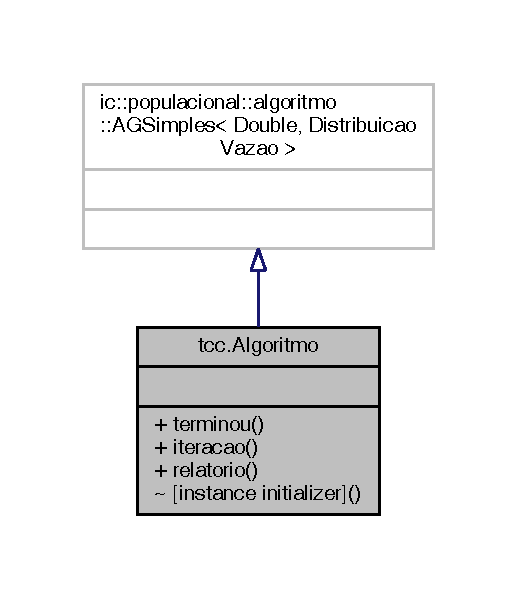
\includegraphics[width=248pt]{classtcc_1_1_algoritmo__inherit__graph}
\end{center}
\end{figure}


Diagrama de colaboração para tcc.\-Algoritmo\-:
\nopagebreak
\begin{figure}[H]
\begin{center}
\leavevmode
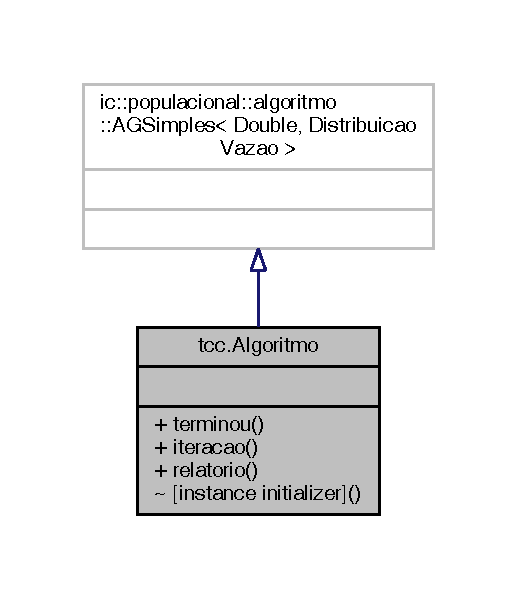
\includegraphics[width=248pt]{classtcc_1_1_algoritmo__coll__graph}
\end{center}
\end{figure}
\subsection*{Métodos Públicos}
\begin{DoxyCompactItemize}
\item 
Boolean \hyperlink{classtcc_1_1_algoritmo_a00f9b2eaaabd5f3bfdd91a4d0511a7d0}{terminou} ()
\item 
void \hyperlink{classtcc_1_1_algoritmo_a762b4fd3ea5f700dfb926cfa6a3c7c53}{iteracao} ()
\item 
String \hyperlink{classtcc_1_1_algoritmo_acca22385ccef352f1b4042100a3b8ba1}{relatorio} ()
\end{DoxyCompactItemize}


\subsection{Descrição Detalhada}
\begin{DoxyAuthor}{Autor}
Victor de Lima Soares 
\end{DoxyAuthor}


\subsection{Métodos}
\hypertarget{classtcc_1_1_algoritmo_a762b4fd3ea5f700dfb926cfa6a3c7c53}{\index{tcc\-::\-Algoritmo@{tcc\-::\-Algoritmo}!iteracao@{iteracao}}
\index{iteracao@{iteracao}!tcc::Algoritmo@{tcc\-::\-Algoritmo}}
\subsubsection[{iteracao}]{\setlength{\rightskip}{0pt plus 5cm}void tcc.\-Algoritmo.\-iteracao (
\begin{DoxyParamCaption}
{}
\end{DoxyParamCaption}
)}}\label{classtcc_1_1_algoritmo_a762b4fd3ea5f700dfb926cfa6a3c7c53}
\hypertarget{classtcc_1_1_algoritmo_acca22385ccef352f1b4042100a3b8ba1}{\index{tcc\-::\-Algoritmo@{tcc\-::\-Algoritmo}!relatorio@{relatorio}}
\index{relatorio@{relatorio}!tcc::Algoritmo@{tcc\-::\-Algoritmo}}
\subsubsection[{relatorio}]{\setlength{\rightskip}{0pt plus 5cm}String tcc.\-Algoritmo.\-relatorio (
\begin{DoxyParamCaption}
{}
\end{DoxyParamCaption}
)}}\label{classtcc_1_1_algoritmo_acca22385ccef352f1b4042100a3b8ba1}
\hypertarget{classtcc_1_1_algoritmo_a00f9b2eaaabd5f3bfdd91a4d0511a7d0}{\index{tcc\-::\-Algoritmo@{tcc\-::\-Algoritmo}!terminou@{terminou}}
\index{terminou@{terminou}!tcc::Algoritmo@{tcc\-::\-Algoritmo}}
\subsubsection[{terminou}]{\setlength{\rightskip}{0pt plus 5cm}Boolean tcc.\-Algoritmo.\-terminou (
\begin{DoxyParamCaption}
{}
\end{DoxyParamCaption}
)}}\label{classtcc_1_1_algoritmo_a00f9b2eaaabd5f3bfdd91a4d0511a7d0}


A documentação para esta classe foi gerada a partir do seguinte arquivo\-:\begin{DoxyCompactItemize}
\item 
C\-:/\-Users/\-Victor/workplace/\-Net\-Beans\-Projects/tcc/src/tcc/\hyperlink{_algoritmo_8java}{Algoritmo.\-java}\end{DoxyCompactItemize}

\hypertarget{classusina_1_1tubulacao_1_1_conduto}{\section{Referência da Classe usina.\-tubulacao.\-Conduto}
\label{classusina_1_1tubulacao_1_1_conduto}\index{usina.\-tubulacao.\-Conduto@{usina.\-tubulacao.\-Conduto}}
}


Diagrama de colaboração para usina.\-tubulacao.\-Conduto\-:
\nopagebreak
\begin{figure}[H]
\begin{center}
\leavevmode
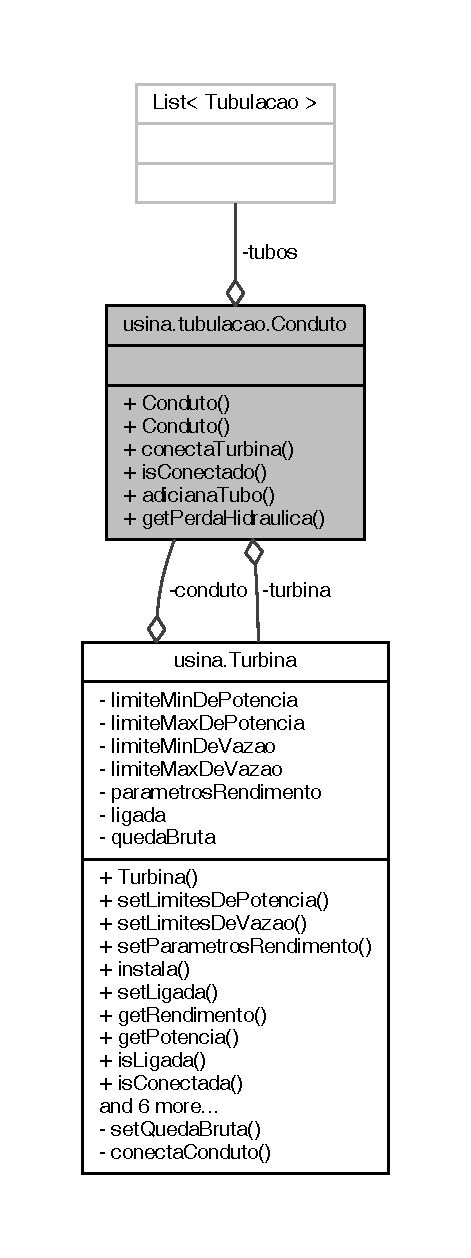
\includegraphics[height=550pt]{classusina_1_1tubulacao_1_1_conduto__coll__graph}
\end{center}
\end{figure}
\subsection*{Métodos Públicos}
\begin{DoxyCompactItemize}
\item 
\hyperlink{classusina_1_1tubulacao_1_1_conduto_a3b4a6577c8557142c06215b9714f60c0}{Conduto} ()
\item 
\hyperlink{classusina_1_1tubulacao_1_1_conduto_a65d6d9d7acde343b6598d090af96acb8}{Conduto} (final Array\-List$<$ Tubulacao $>$ \hyperlink{classusina_1_1tubulacao_1_1_conduto_a0818dcc694d38d10020eb0335e4d44b0}{tubos})
\item 
final void \hyperlink{classusina_1_1tubulacao_1_1_conduto_aa187e888eb82bed03c1485f329f74267}{conecta\-Turbina} (final \hyperlink{classusina_1_1_turbina}{Turbina} \hyperlink{classusina_1_1tubulacao_1_1_conduto_a82d53c81437766af2da7d80771ab5fad}{turbina})
\item 
boolean \hyperlink{classusina_1_1tubulacao_1_1_conduto_a66622b4eb62e7fc446410ef49dda64b5}{is\-Conectado} ()
\item 
final void \hyperlink{classusina_1_1tubulacao_1_1_conduto_a40cfa8928ec6b78584f0dada4e5a40fc}{adiciana\-Tubo} (Tubulacao tubo)
\item 
final double \hyperlink{classusina_1_1tubulacao_1_1_conduto_a2b1644e1a9e6a68245c942aa6e01db59}{get\-Perda\-Hidraulica} (\hyperlink{classusina_1_1_fluxo}{Fluxo} fluxo)
\end{DoxyCompactItemize}
\subsection*{Atributos Privados}
\begin{DoxyCompactItemize}
\item 
final List$<$ Tubulacao $>$ \hyperlink{classusina_1_1tubulacao_1_1_conduto_a0818dcc694d38d10020eb0335e4d44b0}{tubos}
\item 
\hyperlink{classusina_1_1_turbina}{Turbina} \hyperlink{classusina_1_1tubulacao_1_1_conduto_a82d53c81437766af2da7d80771ab5fad}{turbina}
\end{DoxyCompactItemize}


\subsection{Descrição Detalhada}
\begin{DoxyAuthor}{Autor}
Victor de Lima Soares 
\end{DoxyAuthor}
\begin{DoxyVersion}{Versão}
1.\-0 
\end{DoxyVersion}


\subsection{Construtores \& Destrutores}
\hypertarget{classusina_1_1tubulacao_1_1_conduto_a3b4a6577c8557142c06215b9714f60c0}{\index{usina\-::tubulacao\-::\-Conduto@{usina\-::tubulacao\-::\-Conduto}!Conduto@{Conduto}}
\index{Conduto@{Conduto}!usina::tubulacao::Conduto@{usina\-::tubulacao\-::\-Conduto}}
\subsubsection[{Conduto}]{\setlength{\rightskip}{0pt plus 5cm}usina.\-tubulacao.\-Conduto.\-Conduto (
\begin{DoxyParamCaption}
{}
\end{DoxyParamCaption}
)}}\label{classusina_1_1tubulacao_1_1_conduto_a3b4a6577c8557142c06215b9714f60c0}
\hypertarget{classusina_1_1tubulacao_1_1_conduto_a65d6d9d7acde343b6598d090af96acb8}{\index{usina\-::tubulacao\-::\-Conduto@{usina\-::tubulacao\-::\-Conduto}!Conduto@{Conduto}}
\index{Conduto@{Conduto}!usina::tubulacao::Conduto@{usina\-::tubulacao\-::\-Conduto}}
\subsubsection[{Conduto}]{\setlength{\rightskip}{0pt plus 5cm}usina.\-tubulacao.\-Conduto.\-Conduto (
\begin{DoxyParamCaption}
\item[{final Array\-List$<$ Tubulacao $>$}]{tubos}
\end{DoxyParamCaption}
)}}\label{classusina_1_1tubulacao_1_1_conduto_a65d6d9d7acde343b6598d090af96acb8}


\subsection{Métodos}
\hypertarget{classusina_1_1tubulacao_1_1_conduto_a40cfa8928ec6b78584f0dada4e5a40fc}{\index{usina\-::tubulacao\-::\-Conduto@{usina\-::tubulacao\-::\-Conduto}!adiciana\-Tubo@{adiciana\-Tubo}}
\index{adiciana\-Tubo@{adiciana\-Tubo}!usina::tubulacao::Conduto@{usina\-::tubulacao\-::\-Conduto}}
\subsubsection[{adiciana\-Tubo}]{\setlength{\rightskip}{0pt plus 5cm}final void usina.\-tubulacao.\-Conduto.\-adiciana\-Tubo (
\begin{DoxyParamCaption}
\item[{Tubulacao}]{tubo}
\end{DoxyParamCaption}
)}}\label{classusina_1_1tubulacao_1_1_conduto_a40cfa8928ec6b78584f0dada4e5a40fc}
\hypertarget{classusina_1_1tubulacao_1_1_conduto_aa187e888eb82bed03c1485f329f74267}{\index{usina\-::tubulacao\-::\-Conduto@{usina\-::tubulacao\-::\-Conduto}!conecta\-Turbina@{conecta\-Turbina}}
\index{conecta\-Turbina@{conecta\-Turbina}!usina::tubulacao::Conduto@{usina\-::tubulacao\-::\-Conduto}}
\subsubsection[{conecta\-Turbina}]{\setlength{\rightskip}{0pt plus 5cm}final void usina.\-tubulacao.\-Conduto.\-conecta\-Turbina (
\begin{DoxyParamCaption}
\item[{final {\bf Turbina}}]{turbina}
\end{DoxyParamCaption}
)}}\label{classusina_1_1tubulacao_1_1_conduto_aa187e888eb82bed03c1485f329f74267}


Este é o diagrama das funções utilizadas por esta função\-:\nopagebreak
\begin{figure}[H]
\begin{center}
\leavevmode
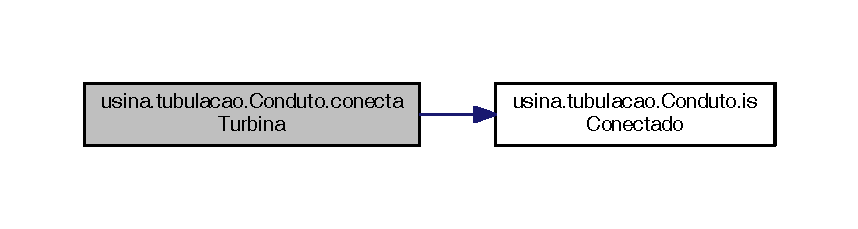
\includegraphics[width=350pt]{classusina_1_1tubulacao_1_1_conduto_aa187e888eb82bed03c1485f329f74267_cgraph}
\end{center}
\end{figure}


\hypertarget{classusina_1_1tubulacao_1_1_conduto_a2b1644e1a9e6a68245c942aa6e01db59}{\index{usina\-::tubulacao\-::\-Conduto@{usina\-::tubulacao\-::\-Conduto}!get\-Perda\-Hidraulica@{get\-Perda\-Hidraulica}}
\index{get\-Perda\-Hidraulica@{get\-Perda\-Hidraulica}!usina::tubulacao::Conduto@{usina\-::tubulacao\-::\-Conduto}}
\subsubsection[{get\-Perda\-Hidraulica}]{\setlength{\rightskip}{0pt plus 5cm}final double usina.\-tubulacao.\-Conduto.\-get\-Perda\-Hidraulica (
\begin{DoxyParamCaption}
\item[{{\bf Fluxo}}]{fluxo}
\end{DoxyParamCaption}
)}}\label{classusina_1_1tubulacao_1_1_conduto_a2b1644e1a9e6a68245c942aa6e01db59}
\hypertarget{classusina_1_1tubulacao_1_1_conduto_a66622b4eb62e7fc446410ef49dda64b5}{\index{usina\-::tubulacao\-::\-Conduto@{usina\-::tubulacao\-::\-Conduto}!is\-Conectado@{is\-Conectado}}
\index{is\-Conectado@{is\-Conectado}!usina::tubulacao::Conduto@{usina\-::tubulacao\-::\-Conduto}}
\subsubsection[{is\-Conectado}]{\setlength{\rightskip}{0pt plus 5cm}boolean usina.\-tubulacao.\-Conduto.\-is\-Conectado (
\begin{DoxyParamCaption}
{}
\end{DoxyParamCaption}
)}}\label{classusina_1_1tubulacao_1_1_conduto_a66622b4eb62e7fc446410ef49dda64b5}


Este é o diagrama das funções que utilizam esta função\-:\nopagebreak
\begin{figure}[H]
\begin{center}
\leavevmode
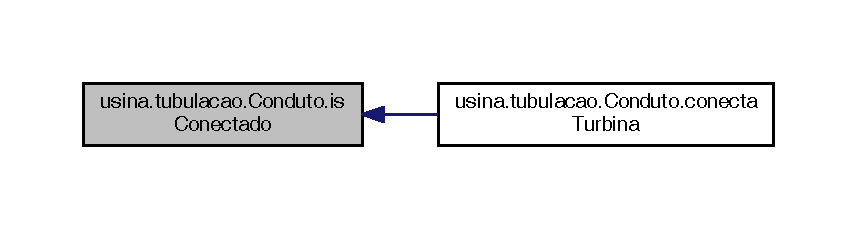
\includegraphics[width=350pt]{classusina_1_1tubulacao_1_1_conduto_a66622b4eb62e7fc446410ef49dda64b5_icgraph}
\end{center}
\end{figure}




\subsection{Atributos}
\hypertarget{classusina_1_1tubulacao_1_1_conduto_a0818dcc694d38d10020eb0335e4d44b0}{\index{usina\-::tubulacao\-::\-Conduto@{usina\-::tubulacao\-::\-Conduto}!tubos@{tubos}}
\index{tubos@{tubos}!usina::tubulacao::Conduto@{usina\-::tubulacao\-::\-Conduto}}
\subsubsection[{tubos}]{\setlength{\rightskip}{0pt plus 5cm}final List$<$Tubulacao$>$ usina.\-tubulacao.\-Conduto.\-tubos\hspace{0.3cm}{\ttfamily [private]}}}\label{classusina_1_1tubulacao_1_1_conduto_a0818dcc694d38d10020eb0335e4d44b0}
\hypertarget{classusina_1_1tubulacao_1_1_conduto_a82d53c81437766af2da7d80771ab5fad}{\index{usina\-::tubulacao\-::\-Conduto@{usina\-::tubulacao\-::\-Conduto}!turbina@{turbina}}
\index{turbina@{turbina}!usina::tubulacao::Conduto@{usina\-::tubulacao\-::\-Conduto}}
\subsubsection[{turbina}]{\setlength{\rightskip}{0pt plus 5cm}{\bf Turbina} usina.\-tubulacao.\-Conduto.\-turbina\hspace{0.3cm}{\ttfamily [private]}}}\label{classusina_1_1tubulacao_1_1_conduto_a82d53c81437766af2da7d80771ab5fad}


A documentação para esta classe foi gerada a partir do seguinte arquivo\-:\begin{DoxyCompactItemize}
\item 
C\-:/\-Users/\-Victor/workplace/\-Net\-Beans\-Projects/tcc/src/usina/tubulacao/\hyperlink{_conduto_8java}{Conduto.\-java}\end{DoxyCompactItemize}

\hypertarget{classusina_1_1tubulacao_1_1_conector_cilindrico_curvo_poligonal}{\section{Referência da Classe usina.\-tubulacao.\-Conector\-Cilindrico\-Curvo\-Poligonal}
\label{classusina_1_1tubulacao_1_1_conector_cilindrico_curvo_poligonal}\index{usina.\-tubulacao.\-Conector\-Cilindrico\-Curvo\-Poligonal@{usina.\-tubulacao.\-Conector\-Cilindrico\-Curvo\-Poligonal}}
}


{\ttfamily Conector} em formato curvo com se��es circulares de mesmo tamanho, e curvatura formada por se��es retas.  




Diagrama de Hierarquia para usina.\-tubulacao.\-Conector\-Cilindrico\-Curvo\-Poligonal\-:
\nopagebreak
\begin{figure}[H]
\begin{center}
\leavevmode
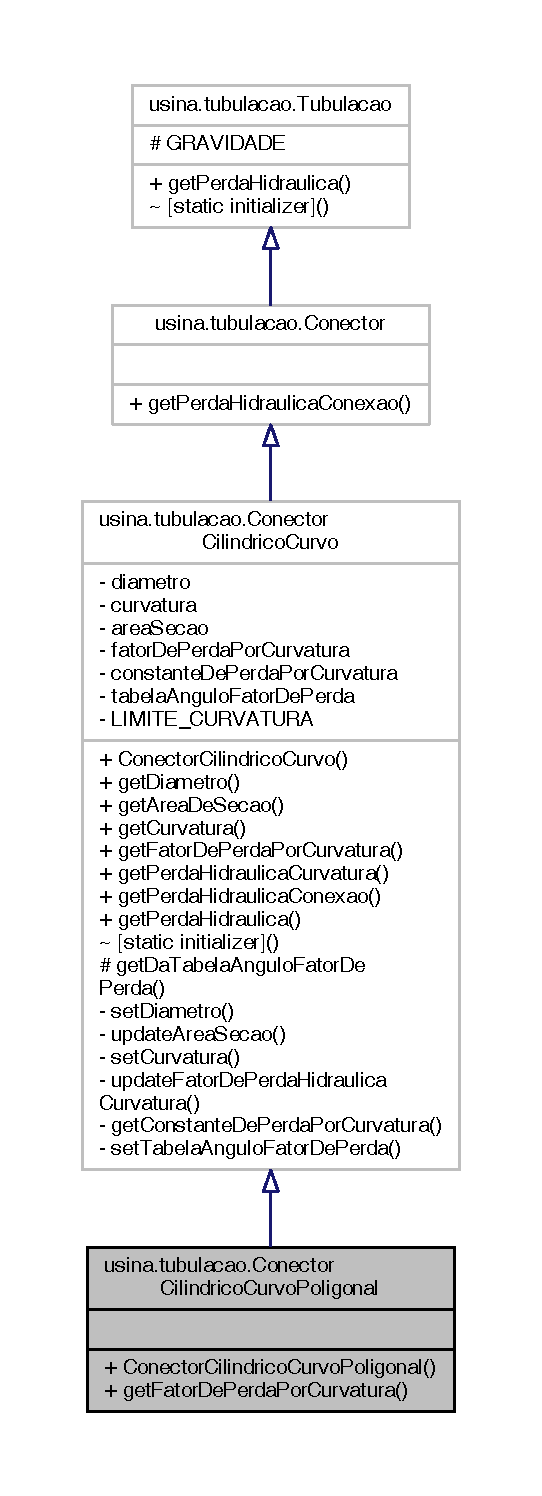
\includegraphics[height=550pt]{classusina_1_1tubulacao_1_1_conector_cilindrico_curvo_poligonal__inherit__graph}
\end{center}
\end{figure}


Diagrama de colaboração para usina.\-tubulacao.\-Conector\-Cilindrico\-Curvo\-Poligonal\-:
\nopagebreak
\begin{figure}[H]
\begin{center}
\leavevmode
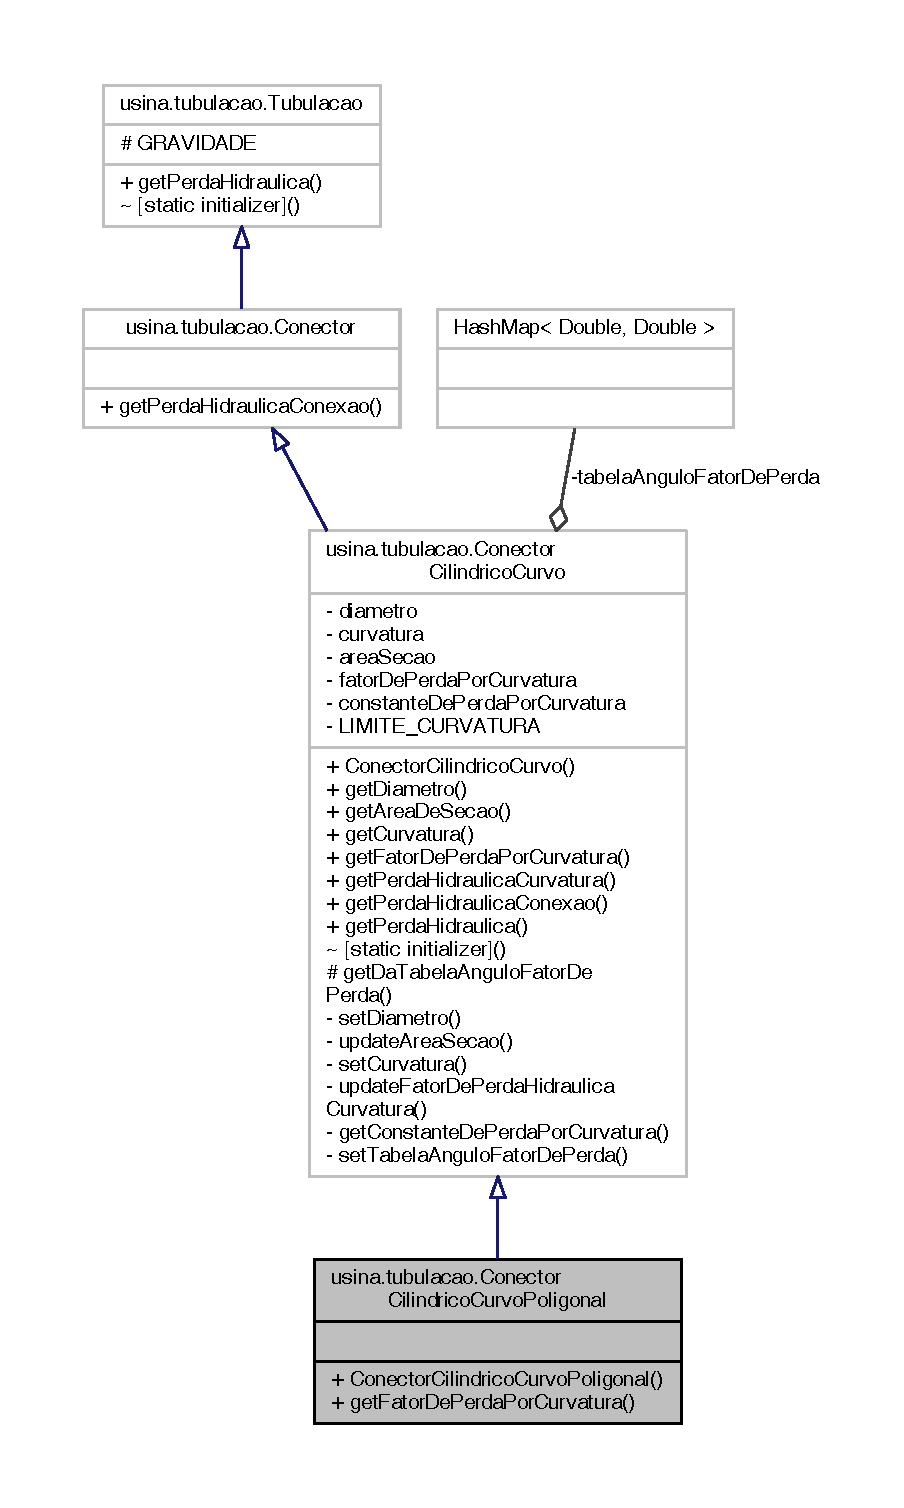
\includegraphics[height=550pt]{classusina_1_1tubulacao_1_1_conector_cilindrico_curvo_poligonal__coll__graph}
\end{center}
\end{figure}
\subsection*{Métodos Públicos}
\begin{DoxyCompactItemize}
\item 
\hyperlink{classusina_1_1tubulacao_1_1_conector_cilindrico_curvo_poligonal_af24992a287a6fb4d6513f2ba2e27fb25}{Conector\-Cilindrico\-Curvo\-Poligonal} (double diametro, double curvatura)
\begin{DoxyCompactList}\small\item\em Construtor. \end{DoxyCompactList}\item 
final double \hyperlink{classusina_1_1tubulacao_1_1_conector_cilindrico_curvo_poligonal_afe1517f6757b99afd227c4a57952e519}{get\-Fator\-De\-Perda\-Por\-Curvatura} (double angulo)
\begin{DoxyCompactList}\small\item\em O\-B\-S\-: Fator de corre��o definido pelo modelo\-: \end{DoxyCompactList}\end{DoxyCompactItemize}


\subsection{Descrição Detalhada}
{\ttfamily Conector} em formato curvo com se��es circulares de mesmo tamanho, e curvatura formada por se��es retas. 

Possui uma única entrada e uma �nica sa�da. 

{\bfseries Limite de curvatura\-: 45 Graus} 

{\bfseries Desvios angulares, considerados pontuais\-: um �nico ponto de desvio.} 

\begin{DoxyAuthor}{Autor}
Victor Soares 
\end{DoxyAuthor}
\begin{DoxyVersion}{Versão}
1.\-0 
\end{DoxyVersion}


\subsection{Construtores \& Destrutores}
\hypertarget{classusina_1_1tubulacao_1_1_conector_cilindrico_curvo_poligonal_af24992a287a6fb4d6513f2ba2e27fb25}{\index{usina\-::tubulacao\-::\-Conector\-Cilindrico\-Curvo\-Poligonal@{usina\-::tubulacao\-::\-Conector\-Cilindrico\-Curvo\-Poligonal}!Conector\-Cilindrico\-Curvo\-Poligonal@{Conector\-Cilindrico\-Curvo\-Poligonal}}
\index{Conector\-Cilindrico\-Curvo\-Poligonal@{Conector\-Cilindrico\-Curvo\-Poligonal}!usina::tubulacao::ConectorCilindricoCurvoPoligonal@{usina\-::tubulacao\-::\-Conector\-Cilindrico\-Curvo\-Poligonal}}
\subsubsection[{Conector\-Cilindrico\-Curvo\-Poligonal}]{\setlength{\rightskip}{0pt plus 5cm}usina.\-tubulacao.\-Conector\-Cilindrico\-Curvo\-Poligonal.\-Conector\-Cilindrico\-Curvo\-Poligonal (
\begin{DoxyParamCaption}
\item[{double}]{diametro, }
\item[{double}]{curvatura}
\end{DoxyParamCaption}
)}}\label{classusina_1_1tubulacao_1_1_conector_cilindrico_curvo_poligonal_af24992a287a6fb4d6513f2ba2e27fb25}


Construtor. 


\begin{DoxyParams}{Parâmetros}
{\em diametro} & Di�metro \mbox{[}m\mbox{]}. \\
\hline
{\em curvatura} & �ngulo de curvatura(desvio) da {\ttfamily tubula��o} \mbox{[}Graus\mbox{]}. \\
\hline
\end{DoxyParams}
\begin{DoxySince}{Desde}
1.\-0 
\end{DoxySince}


\subsection{Métodos}
\hypertarget{classusina_1_1tubulacao_1_1_conector_cilindrico_curvo_poligonal_afe1517f6757b99afd227c4a57952e519}{\index{usina\-::tubulacao\-::\-Conector\-Cilindrico\-Curvo\-Poligonal@{usina\-::tubulacao\-::\-Conector\-Cilindrico\-Curvo\-Poligonal}!get\-Fator\-De\-Perda\-Por\-Curvatura@{get\-Fator\-De\-Perda\-Por\-Curvatura}}
\index{get\-Fator\-De\-Perda\-Por\-Curvatura@{get\-Fator\-De\-Perda\-Por\-Curvatura}!usina::tubulacao::ConectorCilindricoCurvoPoligonal@{usina\-::tubulacao\-::\-Conector\-Cilindrico\-Curvo\-Poligonal}}
\subsubsection[{get\-Fator\-De\-Perda\-Por\-Curvatura}]{\setlength{\rightskip}{0pt plus 5cm}final double usina.\-tubulacao.\-Conector\-Cilindrico\-Curvo\-Poligonal.\-get\-Fator\-De\-Perda\-Por\-Curvatura (
\begin{DoxyParamCaption}
\item[{double}]{angulo}
\end{DoxyParamCaption}
)}}\label{classusina_1_1tubulacao_1_1_conector_cilindrico_curvo_poligonal_afe1517f6757b99afd227c4a57952e519}


O\-B\-S\-: Fator de corre��o definido pelo modelo\-: 


\begin{DoxyItemize}
\item �ngulos de desvio menores ou iguais a 15 Graus\-: 2\% 
\item �ngulos de desvio maiores que 15 Graus\-: 3\% 
\end{DoxyItemize}

A documentação para esta classe foi gerada a partir do seguinte arquivo\-:\begin{DoxyCompactItemize}
\item 
C\-:/\-Users/\-Victor/workplace/\-Net\-Beans\-Projects/tcc/src/usina/tubulacao/\hyperlink{_conector_cilindrico_curvo_poligonal_8java}{Conector\-Cilindrico\-Curvo\-Poligonal.\-java}\end{DoxyCompactItemize}

\hypertarget{classusina_1_1tubulacao_1_1_conector_cilindrico_curvo_suave}{\section{Referência da Classe usina.\-tubulacao.\-Conector\-Cilindrico\-Curvo\-Suave}
\label{classusina_1_1tubulacao_1_1_conector_cilindrico_curvo_suave}\index{usina.\-tubulacao.\-Conector\-Cilindrico\-Curvo\-Suave@{usina.\-tubulacao.\-Conector\-Cilindrico\-Curvo\-Suave}}
}


Conector Cilindrico Curvo Suave.  




Diagrama de Hierarquia para usina.\-tubulacao.\-Conector\-Cilindrico\-Curvo\-Suave\-:
\nopagebreak
\begin{figure}[H]
\begin{center}
\leavevmode
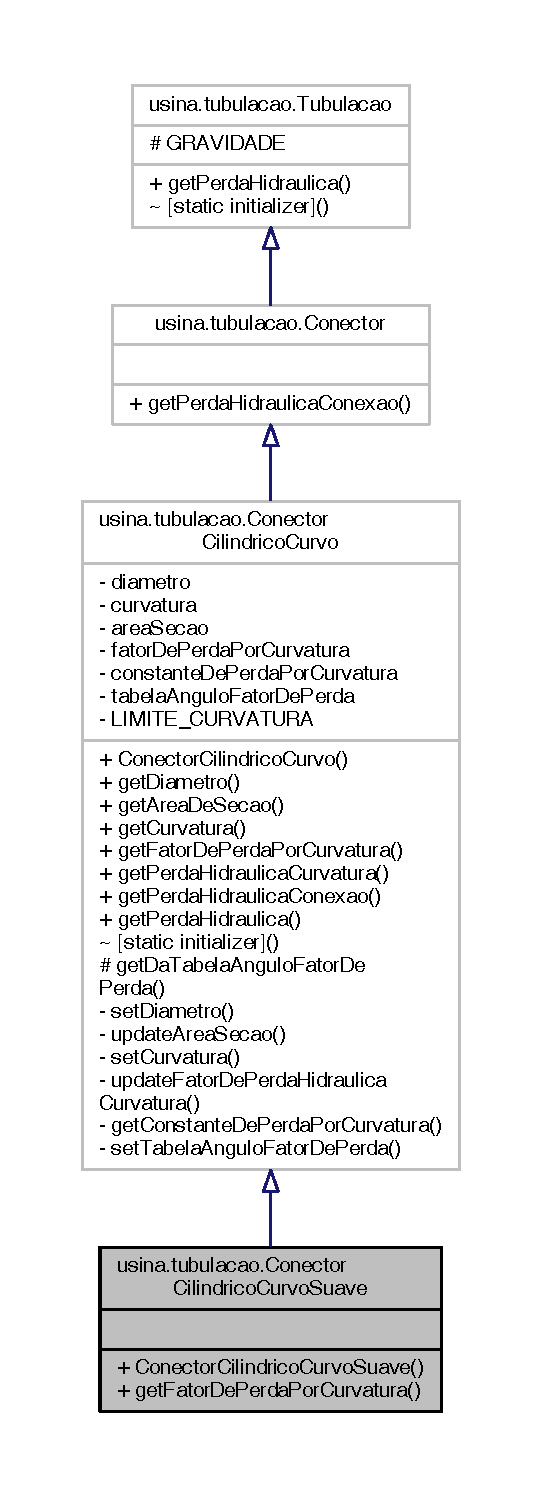
\includegraphics[height=550pt]{classusina_1_1tubulacao_1_1_conector_cilindrico_curvo_suave__inherit__graph}
\end{center}
\end{figure}


Diagrama de colaboração para usina.\-tubulacao.\-Conector\-Cilindrico\-Curvo\-Suave\-:
\nopagebreak
\begin{figure}[H]
\begin{center}
\leavevmode
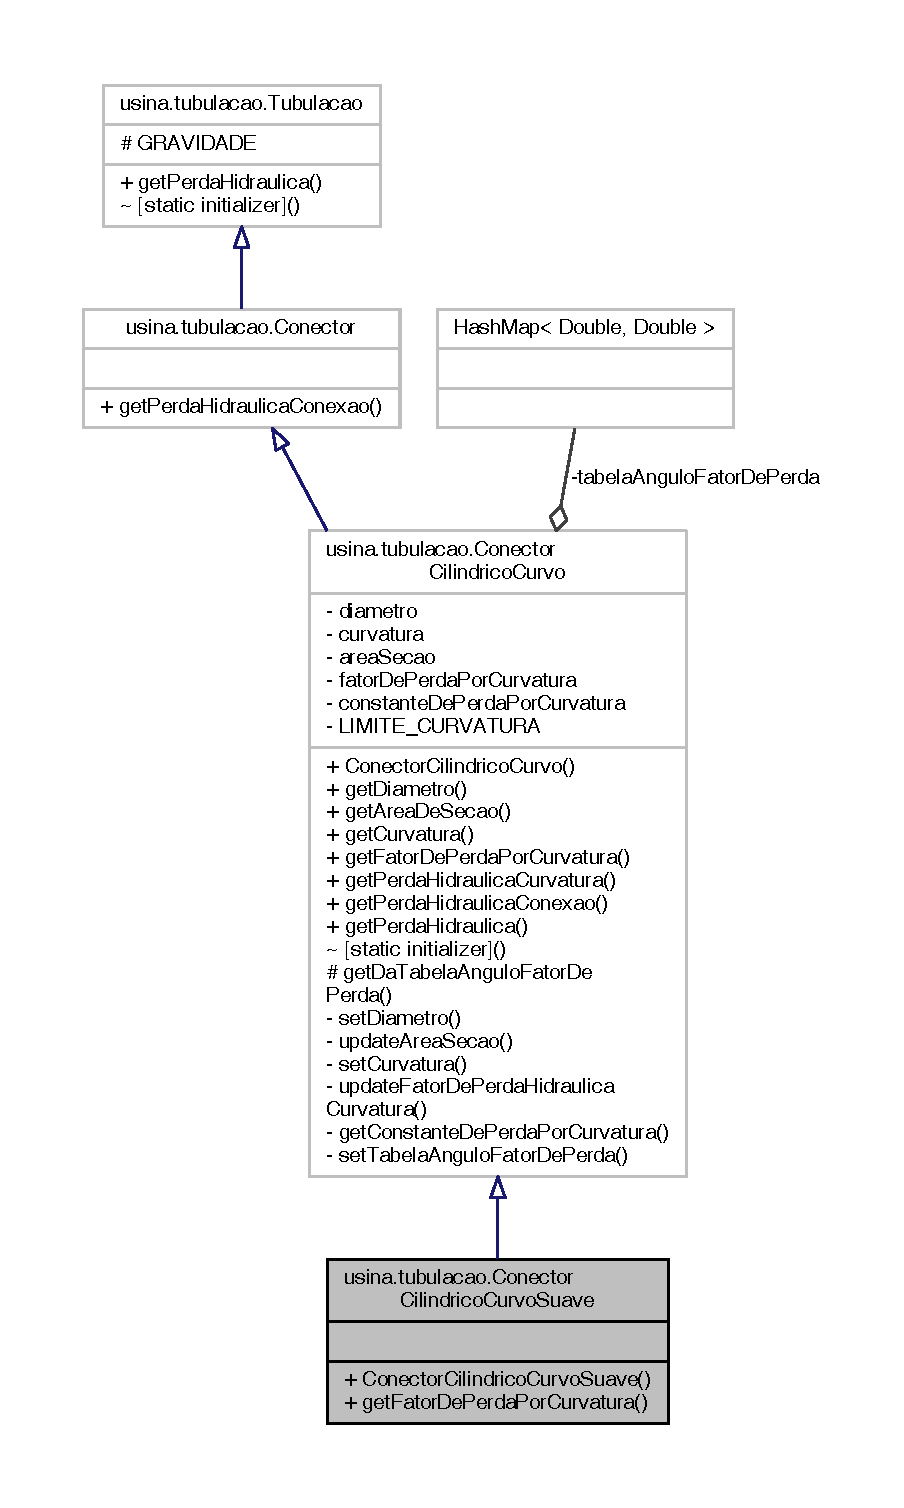
\includegraphics[height=550pt]{classusina_1_1tubulacao_1_1_conector_cilindrico_curvo_suave__coll__graph}
\end{center}
\end{figure}
\subsection*{Métodos Públicos}
\begin{DoxyCompactItemize}
\item 
\hyperlink{classusina_1_1tubulacao_1_1_conector_cilindrico_curvo_suave_a2c8cc6975cd18869d1524a4edc1f19db}{Conector\-Cilindrico\-Curvo\-Suave} (double diametro, double curvatura)
\begin{DoxyCompactList}\small\item\em Construtor. \end{DoxyCompactList}\item 
final double \hyperlink{classusina_1_1tubulacao_1_1_conector_cilindrico_curvo_suave_a6de53dc8bcead270bcfd0a2e5f9a010d}{get\-Fator\-De\-Perda\-Por\-Curvatura} (double angulo)
\end{DoxyCompactItemize}


\subsection{Descrição Detalhada}
Conector Cilindrico Curvo Suave. 

{\ttfamily Conector} em formato curvo com se��es circulares de mesmo di�metro, formando uma curva suave. 

Possui uma �nica entrada e uma �nica sa�da. 

{\bfseries Limite\-: 45 Graus} 

\begin{DoxyAuthor}{Autor}
Victor Soares 
\end{DoxyAuthor}
\begin{DoxyVersion}{Versão}
1.\-0 
\end{DoxyVersion}


\subsection{Construtores \& Destrutores}
\hypertarget{classusina_1_1tubulacao_1_1_conector_cilindrico_curvo_suave_a2c8cc6975cd18869d1524a4edc1f19db}{\index{usina\-::tubulacao\-::\-Conector\-Cilindrico\-Curvo\-Suave@{usina\-::tubulacao\-::\-Conector\-Cilindrico\-Curvo\-Suave}!Conector\-Cilindrico\-Curvo\-Suave@{Conector\-Cilindrico\-Curvo\-Suave}}
\index{Conector\-Cilindrico\-Curvo\-Suave@{Conector\-Cilindrico\-Curvo\-Suave}!usina::tubulacao::ConectorCilindricoCurvoSuave@{usina\-::tubulacao\-::\-Conector\-Cilindrico\-Curvo\-Suave}}
\subsubsection[{Conector\-Cilindrico\-Curvo\-Suave}]{\setlength{\rightskip}{0pt plus 5cm}usina.\-tubulacao.\-Conector\-Cilindrico\-Curvo\-Suave.\-Conector\-Cilindrico\-Curvo\-Suave (
\begin{DoxyParamCaption}
\item[{double}]{diametro, }
\item[{double}]{curvatura}
\end{DoxyParamCaption}
)}}\label{classusina_1_1tubulacao_1_1_conector_cilindrico_curvo_suave_a2c8cc6975cd18869d1524a4edc1f19db}


Construtor. 


\begin{DoxyParams}{Parâmetros}
{\em diametro} & Di�metro \mbox{[}m\mbox{]}. \\
\hline
{\em curvatura} & �ngulo de curvatura(desvio) da {\ttfamily tubula��o} \mbox{[}Graus\mbox{]}. \\
\hline
\end{DoxyParams}
\begin{DoxySince}{Desde}
1.\-0 
\end{DoxySince}


\subsection{Métodos}
\hypertarget{classusina_1_1tubulacao_1_1_conector_cilindrico_curvo_suave_a6de53dc8bcead270bcfd0a2e5f9a010d}{\index{usina\-::tubulacao\-::\-Conector\-Cilindrico\-Curvo\-Suave@{usina\-::tubulacao\-::\-Conector\-Cilindrico\-Curvo\-Suave}!get\-Fator\-De\-Perda\-Por\-Curvatura@{get\-Fator\-De\-Perda\-Por\-Curvatura}}
\index{get\-Fator\-De\-Perda\-Por\-Curvatura@{get\-Fator\-De\-Perda\-Por\-Curvatura}!usina::tubulacao::ConectorCilindricoCurvoSuave@{usina\-::tubulacao\-::\-Conector\-Cilindrico\-Curvo\-Suave}}
\subsubsection[{get\-Fator\-De\-Perda\-Por\-Curvatura}]{\setlength{\rightskip}{0pt plus 5cm}final double usina.\-tubulacao.\-Conector\-Cilindrico\-Curvo\-Suave.\-get\-Fator\-De\-Perda\-Por\-Curvatura (
\begin{DoxyParamCaption}
\item[{double}]{angulo}
\end{DoxyParamCaption}
)}}\label{classusina_1_1tubulacao_1_1_conector_cilindrico_curvo_suave_a6de53dc8bcead270bcfd0a2e5f9a010d}






A documentação para esta classe foi gerada a partir do seguinte arquivo\-:\begin{DoxyCompactItemize}
\item 
C\-:/\-Users/\-Victor/workplace/\-Net\-Beans\-Projects/tcc/src/usina/tubulacao/\hyperlink{_conector_cilindrico_curvo_suave_8java}{Conector\-Cilindrico\-Curvo\-Suave.\-java}\end{DoxyCompactItemize}

\hypertarget{enumusina_1_1_d_a_o_1_1turbina_1_1_tubina_d_a_o_factory_1_1_d_a_o_types}{\section{usina.\-D\-A\-O.\-turbina.\-Tubina\-D\-A\-O\-Factory.\-D\-A\-O\-Types Enum Reference}
\label{enumusina_1_1_d_a_o_1_1turbina_1_1_tubina_d_a_o_factory_1_1_d_a_o_types}\index{usina.\-D\-A\-O.\-turbina.\-Tubina\-D\-A\-O\-Factory.\-D\-A\-O\-Types@{usina.\-D\-A\-O.\-turbina.\-Tubina\-D\-A\-O\-Factory.\-D\-A\-O\-Types}}
}


Diagrama de colaboração para usina.\-D\-A\-O.\-turbina.\-Tubina\-D\-A\-O\-Factory.\-D\-A\-O\-Types\-:\nopagebreak
\begin{figure}[H]
\begin{center}
\leavevmode
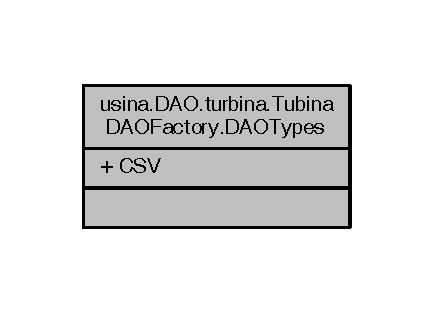
\includegraphics[width=208pt]{enumusina_1_1_d_a_o_1_1turbina_1_1_tubina_d_a_o_factory_1_1_d_a_o_types__coll__graph}
\end{center}
\end{figure}
\subsection*{Atributos Públicos}
\begin{DoxyCompactItemize}
\item 
\hyperlink{enumusina_1_1_d_a_o_1_1turbina_1_1_tubina_d_a_o_factory_1_1_d_a_o_types_a65cd2f40d00a25748553b7c01f8b27a1}{C\-S\-V}
\end{DoxyCompactItemize}


\subsection{Atributos}
\hypertarget{enumusina_1_1_d_a_o_1_1turbina_1_1_tubina_d_a_o_factory_1_1_d_a_o_types_a65cd2f40d00a25748553b7c01f8b27a1}{\index{usina\-::\-D\-A\-O\-::turbina\-::\-Tubina\-D\-A\-O\-Factory\-::\-D\-A\-O\-Types@{usina\-::\-D\-A\-O\-::turbina\-::\-Tubina\-D\-A\-O\-Factory\-::\-D\-A\-O\-Types}!C\-S\-V@{C\-S\-V}}
\index{C\-S\-V@{C\-S\-V}!usina::DAO::turbina::TubinaDAOFactory::DAOTypes@{usina\-::\-D\-A\-O\-::turbina\-::\-Tubina\-D\-A\-O\-Factory\-::\-D\-A\-O\-Types}}
\subsubsection[{C\-S\-V}]{\setlength{\rightskip}{0pt plus 5cm}usina.\-D\-A\-O.\-turbina.\-Tubina\-D\-A\-O\-Factory.\-D\-A\-O\-Types.\-C\-S\-V}}\label{enumusina_1_1_d_a_o_1_1turbina_1_1_tubina_d_a_o_factory_1_1_d_a_o_types_a65cd2f40d00a25748553b7c01f8b27a1}


The documentation for this enum was generated from the following file\-:\begin{DoxyCompactItemize}
\item 
C\-:/\-Users/\-Victor/workplace/\-Net\-Beans\-Projects/tcc/src/usina/\-D\-A\-O/turbina/\hyperlink{_tubina_d_a_o_factory_8java}{Tubina\-D\-A\-O\-Factory.\-java}\end{DoxyCompactItemize}

\hypertarget{classusina_1_1_distribuicao_vazao}{\section{Referência da Classe usina.\-Distribuicao\-Vazao}
\label{classusina_1_1_distribuicao_vazao}\index{usina.\-Distribuicao\-Vazao@{usina.\-Distribuicao\-Vazao}}
}


Distribuição de vazão.  




Diagrama de Hierarquia para usina.\-Distribuicao\-Vazao\-:
\nopagebreak
\begin{figure}[H]
\begin{center}
\leavevmode
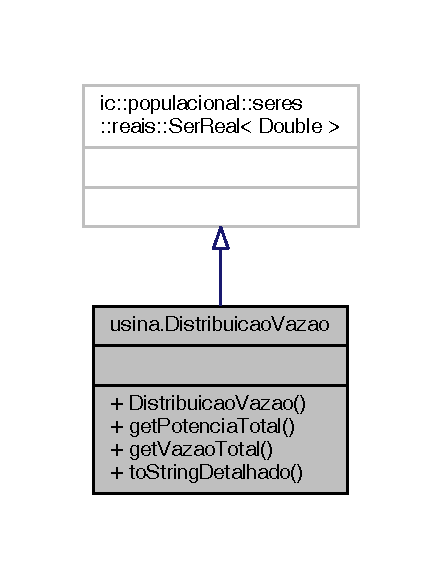
\includegraphics[width=212pt]{classusina_1_1_distribuicao_vazao__inherit__graph}
\end{center}
\end{figure}


Diagrama de colaboração para usina.\-Distribuicao\-Vazao\-:
\nopagebreak
\begin{figure}[H]
\begin{center}
\leavevmode
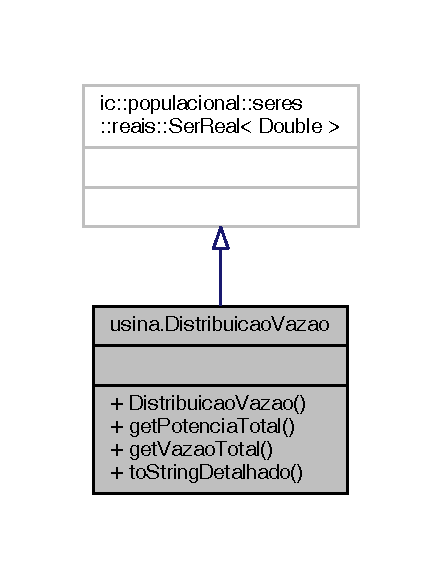
\includegraphics[width=212pt]{classusina_1_1_distribuicao_vazao__coll__graph}
\end{center}
\end{figure}
\subsection*{Métodos Públicos}
\begin{DoxyCompactItemize}
\item 
\hyperlink{classusina_1_1_distribuicao_vazao_ac0e92594534527991f4f00240732e6a5}{Distribuicao\-Vazao} (Integer n\-Vazoes)
\item 
Double \hyperlink{classusina_1_1_distribuicao_vazao_afe121af5937973e50d18126a60293771}{get\-Potencia\-Total} ()
\begin{DoxyCompactList}\small\item\em Retorna a soma das potências geradas pelas turbinas. \end{DoxyCompactList}\item 
Double \hyperlink{classusina_1_1_distribuicao_vazao_ad34a5a0175ac8ed7c2fffc57b2fb325e}{get\-Vazao\-Total} ()
\begin{DoxyCompactList}\small\item\em Retorna a soma das vazões geradas pelas turbinas. \end{DoxyCompactList}\item 
String \hyperlink{classusina_1_1_distribuicao_vazao_a3fe3a91243c236757535a001afaf2aa3}{to\-String\-Detalhado} ()
\end{DoxyCompactItemize}


\subsection{Descrição Detalhada}
Distribuição de vazão. 

Essa classe representa a distribuição de vazão entre os conjuntos turbinas que compõem o sistema, sendo portanto o alvo dos algoritmos evolucionários que tratam do problema do despacho elétrico. 

Cada distribuição agrupa em si um conjunto de características reais, que representam uma vazão para uma determinada turbina. 

\begin{DoxyAuthor}{Autor}
Victor de Lima Soares
\end{DoxyAuthor}
\begin{DoxyVersion}{Versão}
1.\-0 
\end{DoxyVersion}
\begin{DoxySeeAlso}{Veja também}
Ser\-Real 
\end{DoxySeeAlso}


\subsection{Construtores \& Destrutores}
\hypertarget{classusina_1_1_distribuicao_vazao_ac0e92594534527991f4f00240732e6a5}{\index{usina\-::\-Distribuicao\-Vazao@{usina\-::\-Distribuicao\-Vazao}!Distribuicao\-Vazao@{Distribuicao\-Vazao}}
\index{Distribuicao\-Vazao@{Distribuicao\-Vazao}!usina::DistribuicaoVazao@{usina\-::\-Distribuicao\-Vazao}}
\subsubsection[{Distribuicao\-Vazao}]{\setlength{\rightskip}{0pt plus 5cm}usina.\-Distribuicao\-Vazao.\-Distribuicao\-Vazao (
\begin{DoxyParamCaption}
\item[{Integer}]{n\-Vazoes}
\end{DoxyParamCaption}
)}}\label{classusina_1_1_distribuicao_vazao_ac0e92594534527991f4f00240732e6a5}


\subsection{Métodos}
\hypertarget{classusina_1_1_distribuicao_vazao_afe121af5937973e50d18126a60293771}{\index{usina\-::\-Distribuicao\-Vazao@{usina\-::\-Distribuicao\-Vazao}!get\-Potencia\-Total@{get\-Potencia\-Total}}
\index{get\-Potencia\-Total@{get\-Potencia\-Total}!usina::DistribuicaoVazao@{usina\-::\-Distribuicao\-Vazao}}
\subsubsection[{get\-Potencia\-Total}]{\setlength{\rightskip}{0pt plus 5cm}Double usina.\-Distribuicao\-Vazao.\-get\-Potencia\-Total (
\begin{DoxyParamCaption}
{}
\end{DoxyParamCaption}
)}}\label{classusina_1_1_distribuicao_vazao_afe121af5937973e50d18126a60293771}


Retorna a soma das potências geradas pelas turbinas. 

\begin{DoxySince}{Desde}
1.\-0 
\end{DoxySince}
\begin{DoxyReturn}{Retorna}
Potência total. 
\end{DoxyReturn}


Este é o diagrama das funções que utilizam esta função\-:
\nopagebreak
\begin{figure}[H]
\begin{center}
\leavevmode
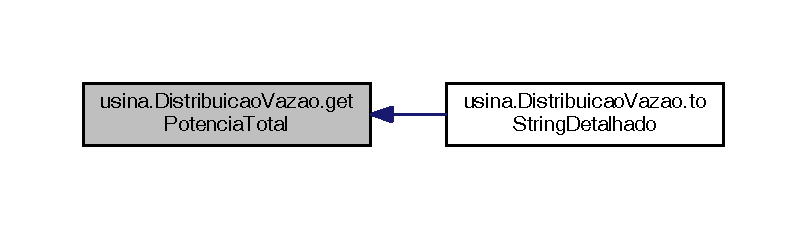
\includegraphics[width=350pt]{classusina_1_1_distribuicao_vazao_afe121af5937973e50d18126a60293771_icgraph}
\end{center}
\end{figure}


\hypertarget{classusina_1_1_distribuicao_vazao_ad34a5a0175ac8ed7c2fffc57b2fb325e}{\index{usina\-::\-Distribuicao\-Vazao@{usina\-::\-Distribuicao\-Vazao}!get\-Vazao\-Total@{get\-Vazao\-Total}}
\index{get\-Vazao\-Total@{get\-Vazao\-Total}!usina::DistribuicaoVazao@{usina\-::\-Distribuicao\-Vazao}}
\subsubsection[{get\-Vazao\-Total}]{\setlength{\rightskip}{0pt plus 5cm}Double usina.\-Distribuicao\-Vazao.\-get\-Vazao\-Total (
\begin{DoxyParamCaption}
{}
\end{DoxyParamCaption}
)}}\label{classusina_1_1_distribuicao_vazao_ad34a5a0175ac8ed7c2fffc57b2fb325e}


Retorna a soma das vazões geradas pelas turbinas. 

\begin{DoxySince}{Desde}
1.\-0 
\end{DoxySince}
\begin{DoxyReturn}{Retorna}
Vazão total. 
\end{DoxyReturn}


Este é o diagrama das funções que utilizam esta função\-:
\nopagebreak
\begin{figure}[H]
\begin{center}
\leavevmode
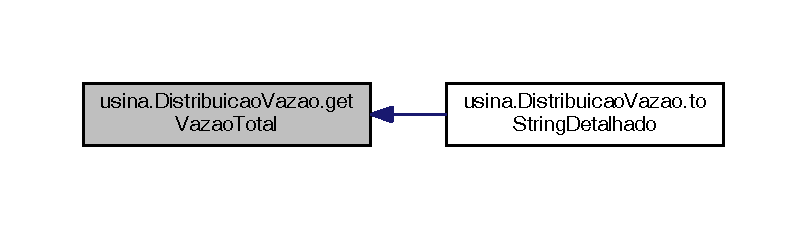
\includegraphics[width=350pt]{classusina_1_1_distribuicao_vazao_ad34a5a0175ac8ed7c2fffc57b2fb325e_icgraph}
\end{center}
\end{figure}


\hypertarget{classusina_1_1_distribuicao_vazao_a3fe3a91243c236757535a001afaf2aa3}{\index{usina\-::\-Distribuicao\-Vazao@{usina\-::\-Distribuicao\-Vazao}!to\-String\-Detalhado@{to\-String\-Detalhado}}
\index{to\-String\-Detalhado@{to\-String\-Detalhado}!usina::DistribuicaoVazao@{usina\-::\-Distribuicao\-Vazao}}
\subsubsection[{to\-String\-Detalhado}]{\setlength{\rightskip}{0pt plus 5cm}String usina.\-Distribuicao\-Vazao.\-to\-String\-Detalhado (
\begin{DoxyParamCaption}
{}
\end{DoxyParamCaption}
)}}\label{classusina_1_1_distribuicao_vazao_a3fe3a91243c236757535a001afaf2aa3}


Este é o diagrama das funções utilizadas por esta função\-:
\nopagebreak
\begin{figure}[H]
\begin{center}
\leavevmode
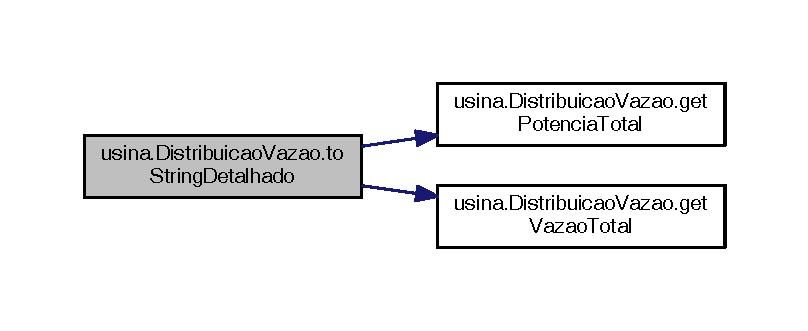
\includegraphics[width=350pt]{classusina_1_1_distribuicao_vazao_a3fe3a91243c236757535a001afaf2aa3_cgraph}
\end{center}
\end{figure}




A documentação para esta classe foi gerada a partir do seguinte arquivo\-:\begin{DoxyCompactItemize}
\item 
C\-:/\-Users/\-Victor/workplace/\-Net\-Beans\-Projects/tcc/src/usina/\hyperlink{_distribuicao_vazao_8java}{Distribuicao\-Vazao.\-java}\end{DoxyCompactItemize}

\hypertarget{classusina_1_1_fluxo}{\section{Referência da Classe usina.\-Fluxo}
\label{classusina_1_1_fluxo}\index{usina.\-Fluxo@{usina.\-Fluxo}}
}


\hyperlink{classusina_1_1_fluxo}{Fluxo}.  




Diagrama de Hierarquia para usina.\-Fluxo\-:
\nopagebreak
\begin{figure}[H]
\begin{center}
\leavevmode
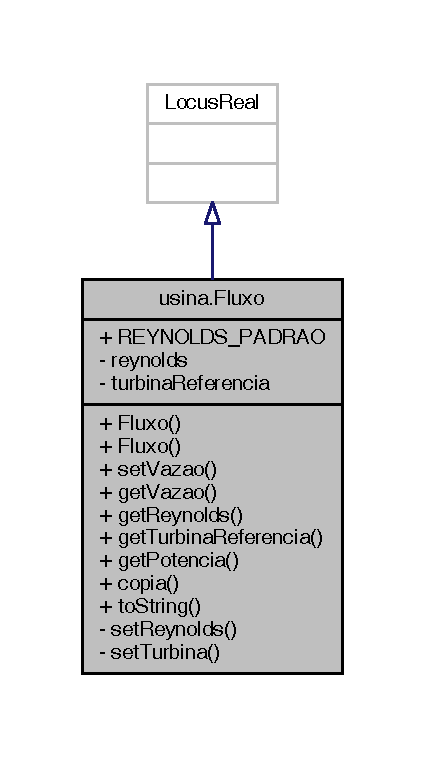
\includegraphics[width=204pt]{classusina_1_1_fluxo__inherit__graph}
\end{center}
\end{figure}


Diagrama de colaboração para usina.\-Fluxo\-:
\nopagebreak
\begin{figure}[H]
\begin{center}
\leavevmode
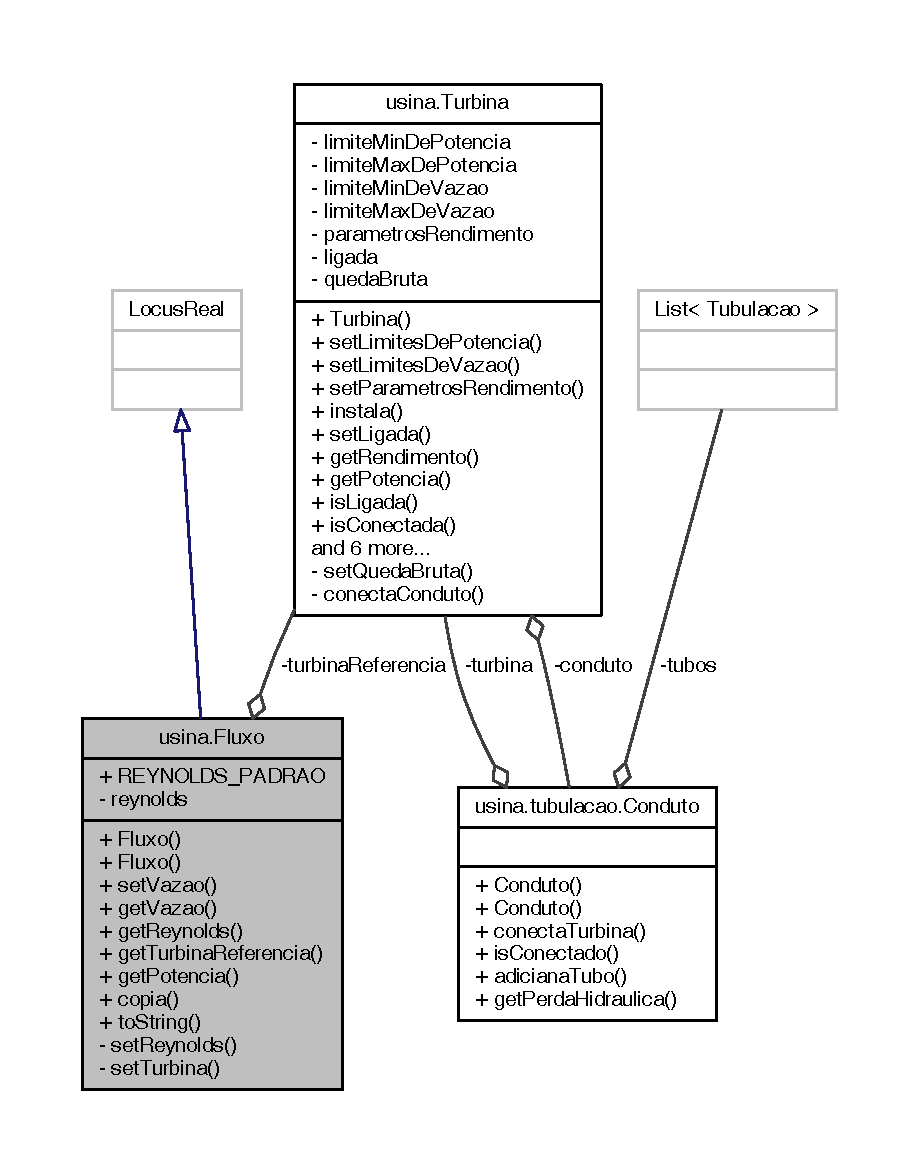
\includegraphics[width=350pt]{classusina_1_1_fluxo__coll__graph}
\end{center}
\end{figure}
\subsection*{Métodos Públicos}
\begin{DoxyCompactItemize}
\item 
\hyperlink{classusina_1_1_fluxo_ab85463cd78cac200be698b91c6be1141}{Fluxo} (Double vazao, \hyperlink{classusina_1_1_turbina}{Turbina} turbina)
\begin{DoxyCompactList}\small\item\em Construtor com Reynolds padrão. \end{DoxyCompactList}\item 
\hyperlink{classusina_1_1_fluxo_a8959019b735089b6cbb96107ba3929b9}{Fluxo} (Double vazao, Double \hyperlink{classusina_1_1_fluxo_a185fed046eefce4fa8f8bb10fde8296d}{reynolds}, \hyperlink{classusina_1_1_turbina}{Turbina} turbina)
\begin{DoxyCompactList}\small\item\em Construtor detalhado. \end{DoxyCompactList}\item 
final void \hyperlink{classusina_1_1_fluxo_af80f13f4ade8128bac424b456ec0836a}{set\-Vazao} (Double vazao)
\begin{DoxyCompactList}\small\item\em Atribui um novo valor de vazão ao fluxo. \end{DoxyCompactList}\item 
final double \hyperlink{classusina_1_1_fluxo_a0634c81d7575ad63274828d8c40a88e5}{get\-Vazao} ()
\begin{DoxyCompactList}\small\item\em Recupera o valor da vazão do fluxo. \end{DoxyCompactList}\item 
final Double \hyperlink{classusina_1_1_fluxo_a110ca81bcee4d7f8f08298b3b9372d21}{get\-Reynolds} ()
\begin{DoxyCompactList}\small\item\em Recupera o número de Reynolds usado. \end{DoxyCompactList}\item 
final \hyperlink{classusina_1_1_turbina}{Turbina} \hyperlink{classusina_1_1_fluxo_a61cc464f6926c453c51fcded2d57306d}{get\-Turbina\-Referencia} ()
\begin{DoxyCompactList}\small\item\em Recupera a turbina da referência. \end{DoxyCompactList}\item 
final Double \hyperlink{classusina_1_1_fluxo_a767621d68cb2ceb8dbbd03bacba8cba5}{get\-Potencia} ()
\begin{DoxyCompactList}\small\item\em Retorna a potência gerada pelo fluxo na turbina. \end{DoxyCompactList}\item 
final \hyperlink{classusina_1_1_fluxo}{Fluxo} \hyperlink{classusina_1_1_fluxo_a9749f0c9449677337f81f1f193d4f564}{copia} ()
\item 
String \hyperlink{classusina_1_1_fluxo_aa7c07414a1af3c807312950fa5019591}{to\-String} ()
\end{DoxyCompactItemize}
\subsection*{Atributos Estáticos Públicos}
\begin{DoxyCompactItemize}
\item 
static final Double \hyperlink{classusina_1_1_fluxo_ad85aeeb220a6c87764d29ce36bb8cc26}{R\-E\-Y\-N\-O\-L\-D\-S\-\_\-\-P\-A\-D\-R\-A\-O} = 70000.\-0
\end{DoxyCompactItemize}
\subsection*{Métodos Privados}
\begin{DoxyCompactItemize}
\item 
void \hyperlink{classusina_1_1_fluxo_a1c204862a651d75929b078355b512823}{set\-Reynolds} (Double \hyperlink{classusina_1_1_fluxo_a185fed046eefce4fa8f8bb10fde8296d}{reynolds})
\begin{DoxyCompactList}\small\item\em Atribui um número de Reynolds ao fluxo. \end{DoxyCompactList}\item 
void \hyperlink{classusina_1_1_fluxo_a3bb30b3608a7ab915ff332018a18d81f}{set\-Turbina} (\hyperlink{classusina_1_1_turbina}{Turbina} \hyperlink{classusina_1_1_fluxo_aee04932f02b1bfad1bf79cc80a1df203}{turbina\-Referencia})
\begin{DoxyCompactList}\small\item\em Atribui uma turbina de referência ao fluxo. \end{DoxyCompactList}\end{DoxyCompactItemize}
\subsection*{Atributos Privados}
\begin{DoxyCompactItemize}
\item 
Double \hyperlink{classusina_1_1_fluxo_a185fed046eefce4fa8f8bb10fde8296d}{reynolds}
\item 
\hyperlink{classusina_1_1_turbina}{Turbina} \hyperlink{classusina_1_1_fluxo_aee04932f02b1bfad1bf79cc80a1df203}{turbina\-Referencia}
\end{DoxyCompactItemize}


\subsection{Descrição Detalhada}
\hyperlink{classusina_1_1_fluxo}{Fluxo}. 

Essa classe representa uma abstração do conceito de fluxo, armazenado em si o valor de uma vazão, seu número de Reynolds e a turbina que o contém,enquanto, permitindo a manipulação dos dados referentes a vazão de modo seguro -\/ respeitando os limites impostos pela turbina. 

Objetos da classe {\ttfamily \hyperlink{classusina_1_1_fluxo}{Fluxo}} indicarão a qual gerador pertencem, compondo facilmente distribuições de fluxo, sem necessidade de que objetos da classe {\ttfamily \hyperlink{classusina_1_1_turbina}{Turbina}} sejam criados mais de uma vez em uma usina. 

Adicionalmente, referências indicando a turbina a qual se refere o fluxo são usadas para verificação dos intervalos de entrada, vazão, ditados pela capacidade de cada turbina. 

A classe estende a a classe {\ttfamily Locus\-Real}, o que a torna passível de utilização em algoritmos evolucionários como característica de um ser baseado em valores reais. 

\begin{DoxyAuthor}{Autor}
Victor Soares 
\end{DoxyAuthor}
\begin{DoxyVersion}{Versão}
1.\-0
\end{DoxyVersion}
\begin{DoxySeeAlso}{Veja também}
Ser\-Real 

Locus\-Real 
\end{DoxySeeAlso}


\subsection{Construtores \& Destrutores}
\hypertarget{classusina_1_1_fluxo_ab85463cd78cac200be698b91c6be1141}{\index{usina\-::\-Fluxo@{usina\-::\-Fluxo}!Fluxo@{Fluxo}}
\index{Fluxo@{Fluxo}!usina::Fluxo@{usina\-::\-Fluxo}}
\subsubsection[{Fluxo}]{\setlength{\rightskip}{0pt plus 5cm}usina.\-Fluxo.\-Fluxo (
\begin{DoxyParamCaption}
\item[{Double}]{vazao, }
\item[{{\bf Turbina}}]{turbina}
\end{DoxyParamCaption}
)}}\label{classusina_1_1_fluxo_ab85463cd78cac200be698b91c6be1141}


Construtor com Reynolds padrão. 

Reynolds padrão\-: 70000. 

\begin{DoxySince}{Desde}
1.\-0 
\end{DoxySince}

\begin{DoxyParams}{Parâmetros}
{\em vazao} & Valor da vazão. \\
\hline
{\em turbina} & \hyperlink{classusina_1_1_turbina}{Turbina} de referência. \\
\hline
\end{DoxyParams}


Este é o diagrama das funções utilizadas por esta função\-:\nopagebreak
\begin{figure}[H]
\begin{center}
\leavevmode
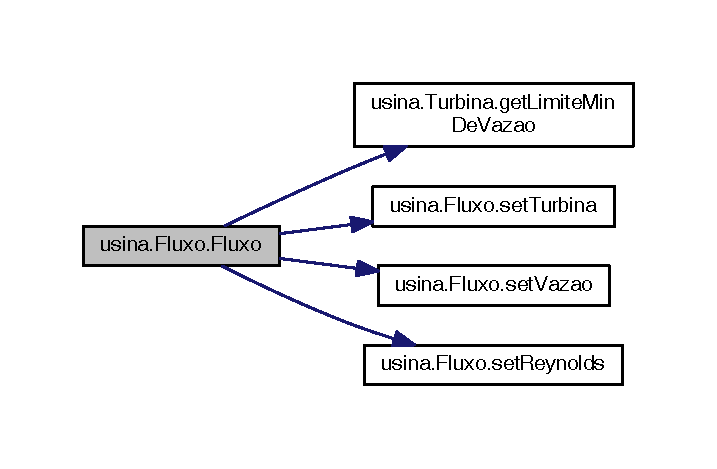
\includegraphics[width=344pt]{classusina_1_1_fluxo_ab85463cd78cac200be698b91c6be1141_cgraph}
\end{center}
\end{figure}




Este é o diagrama das funções que utilizam esta função\-:\nopagebreak
\begin{figure}[H]
\begin{center}
\leavevmode
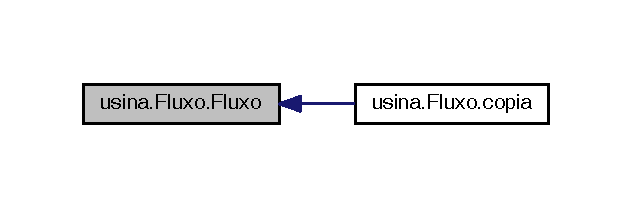
\includegraphics[width=304pt]{classusina_1_1_fluxo_ab85463cd78cac200be698b91c6be1141_icgraph}
\end{center}
\end{figure}


\hypertarget{classusina_1_1_fluxo_a8959019b735089b6cbb96107ba3929b9}{\index{usina\-::\-Fluxo@{usina\-::\-Fluxo}!Fluxo@{Fluxo}}
\index{Fluxo@{Fluxo}!usina::Fluxo@{usina\-::\-Fluxo}}
\subsubsection[{Fluxo}]{\setlength{\rightskip}{0pt plus 5cm}usina.\-Fluxo.\-Fluxo (
\begin{DoxyParamCaption}
\item[{Double}]{vazao, }
\item[{Double}]{reynolds, }
\item[{{\bf Turbina}}]{turbina}
\end{DoxyParamCaption}
)}}\label{classusina_1_1_fluxo_a8959019b735089b6cbb96107ba3929b9}


Construtor detalhado. 

\begin{DoxySince}{Desde}
1.\-0 
\end{DoxySince}

\begin{DoxyParams}{Parâmetros}
{\em vazao} & Valor da vazão. \\
\hline
{\em reynolds} & Número de Reynolds. \\
\hline
{\em turbina} & \hyperlink{classusina_1_1_turbina}{Turbina} de referência. \\
\hline
\end{DoxyParams}


Este é o diagrama das funções utilizadas por esta função\-:\nopagebreak
\begin{figure}[H]
\begin{center}
\leavevmode
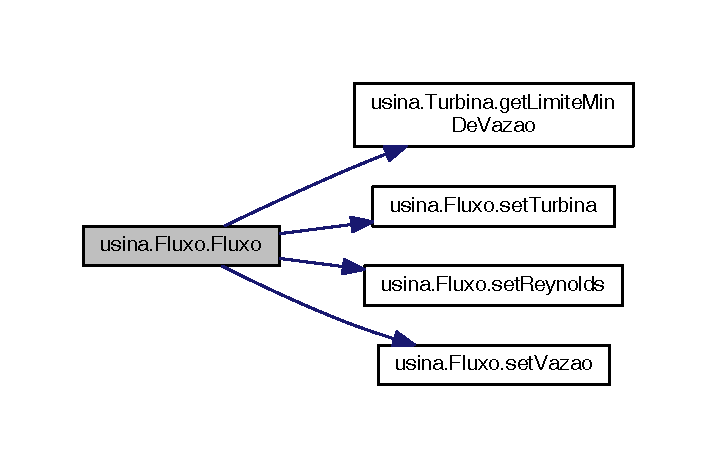
\includegraphics[width=344pt]{classusina_1_1_fluxo_a8959019b735089b6cbb96107ba3929b9_cgraph}
\end{center}
\end{figure}




\subsection{Métodos}
\hypertarget{classusina_1_1_fluxo_a9749f0c9449677337f81f1f193d4f564}{\index{usina\-::\-Fluxo@{usina\-::\-Fluxo}!copia@{copia}}
\index{copia@{copia}!usina::Fluxo@{usina\-::\-Fluxo}}
\subsubsection[{copia}]{\setlength{\rightskip}{0pt plus 5cm}final {\bf Fluxo} usina.\-Fluxo.\-copia (
\begin{DoxyParamCaption}
{}
\end{DoxyParamCaption}
)}}\label{classusina_1_1_fluxo_a9749f0c9449677337f81f1f193d4f564}


Este é o diagrama das funções utilizadas por esta função\-:\nopagebreak
\begin{figure}[H]
\begin{center}
\leavevmode
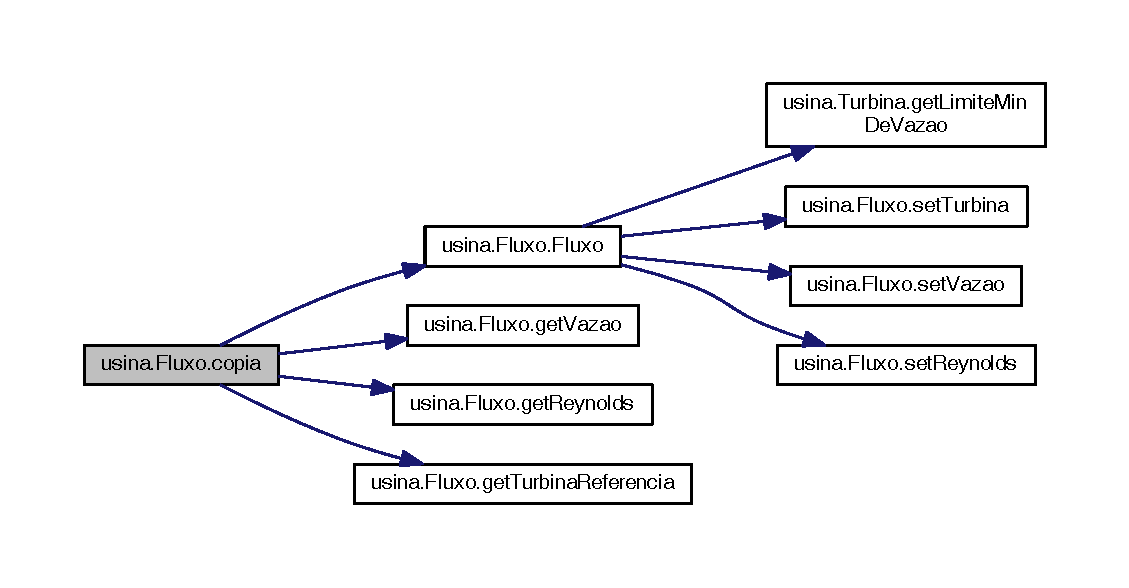
\includegraphics[width=350pt]{classusina_1_1_fluxo_a9749f0c9449677337f81f1f193d4f564_cgraph}
\end{center}
\end{figure}


\hypertarget{classusina_1_1_fluxo_a767621d68cb2ceb8dbbd03bacba8cba5}{\index{usina\-::\-Fluxo@{usina\-::\-Fluxo}!get\-Potencia@{get\-Potencia}}
\index{get\-Potencia@{get\-Potencia}!usina::Fluxo@{usina\-::\-Fluxo}}
\subsubsection[{get\-Potencia}]{\setlength{\rightskip}{0pt plus 5cm}final Double usina.\-Fluxo.\-get\-Potencia (
\begin{DoxyParamCaption}
{}
\end{DoxyParamCaption}
)}}\label{classusina_1_1_fluxo_a767621d68cb2ceb8dbbd03bacba8cba5}


Retorna a potência gerada pelo fluxo na turbina. 

Método de atalho para \hyperlink{classusina_1_1_turbina_ab5f2692c54cf1e3fe6b30adc3b481710}{Turbina\#get\-Potencia(usina.\-Fluxo)}, tendo esse fluxo como parâmetro. 

\begin{DoxySince}{Desde}
1.\-0 
\end{DoxySince}
\begin{DoxyReturn}{Retorna}
Potência da turbina. 
\end{DoxyReturn}
\begin{DoxySeeAlso}{Veja também}
\hyperlink{classusina_1_1_turbina_ab5f2692c54cf1e3fe6b30adc3b481710}{Turbina\-::get\-Potencia}(\hyperlink{classusina_1_1_fluxo}{usina.\-Fluxo}) 
\end{DoxySeeAlso}


Este é o diagrama das funções utilizadas por esta função\-:
\nopagebreak
\begin{figure}[H]
\begin{center}
\leavevmode
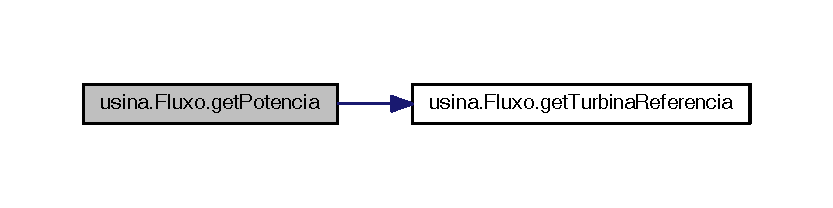
\includegraphics[width=350pt]{classusina_1_1_fluxo_a767621d68cb2ceb8dbbd03bacba8cba5_cgraph}
\end{center}
\end{figure}




Este é o diagrama das funções que utilizam esta função\-:
\nopagebreak
\begin{figure}[H]
\begin{center}
\leavevmode
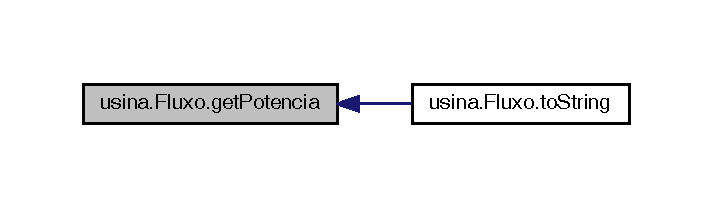
\includegraphics[width=342pt]{classusina_1_1_fluxo_a767621d68cb2ceb8dbbd03bacba8cba5_icgraph}
\end{center}
\end{figure}


\hypertarget{classusina_1_1_fluxo_a110ca81bcee4d7f8f08298b3b9372d21}{\index{usina\-::\-Fluxo@{usina\-::\-Fluxo}!get\-Reynolds@{get\-Reynolds}}
\index{get\-Reynolds@{get\-Reynolds}!usina::Fluxo@{usina\-::\-Fluxo}}
\subsubsection[{get\-Reynolds}]{\setlength{\rightskip}{0pt plus 5cm}final Double usina.\-Fluxo.\-get\-Reynolds (
\begin{DoxyParamCaption}
{}
\end{DoxyParamCaption}
)}}\label{classusina_1_1_fluxo_a110ca81bcee4d7f8f08298b3b9372d21}


Recupera o número de Reynolds usado. 

\begin{DoxySince}{Desde}
1.\-0 
\end{DoxySince}
\begin{DoxyReturn}{Retorna}
O número de Reynolds. 
\end{DoxyReturn}


Este é o diagrama das funções que utilizam esta função\-:\nopagebreak
\begin{figure}[H]
\begin{center}
\leavevmode
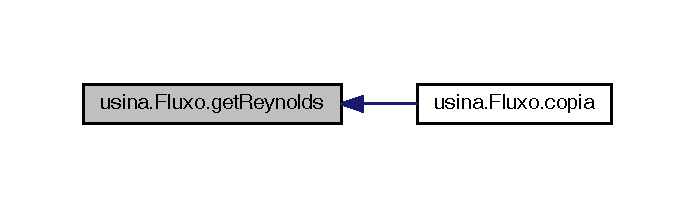
\includegraphics[width=334pt]{classusina_1_1_fluxo_a110ca81bcee4d7f8f08298b3b9372d21_icgraph}
\end{center}
\end{figure}


\hypertarget{classusina_1_1_fluxo_a61cc464f6926c453c51fcded2d57306d}{\index{usina\-::\-Fluxo@{usina\-::\-Fluxo}!get\-Turbina\-Referencia@{get\-Turbina\-Referencia}}
\index{get\-Turbina\-Referencia@{get\-Turbina\-Referencia}!usina::Fluxo@{usina\-::\-Fluxo}}
\subsubsection[{get\-Turbina\-Referencia}]{\setlength{\rightskip}{0pt plus 5cm}final {\bf Turbina} usina.\-Fluxo.\-get\-Turbina\-Referencia (
\begin{DoxyParamCaption}
{}
\end{DoxyParamCaption}
)}}\label{classusina_1_1_fluxo_a61cc464f6926c453c51fcded2d57306d}


Recupera a turbina da referência. 

\begin{DoxySince}{Desde}
1.\-0 
\end{DoxySince}
\begin{DoxyReturn}{Retorna}
A turbina de Referencia 
\end{DoxyReturn}


Este é o diagrama das funções que utilizam esta função\-:
\nopagebreak
\begin{figure}[H]
\begin{center}
\leavevmode
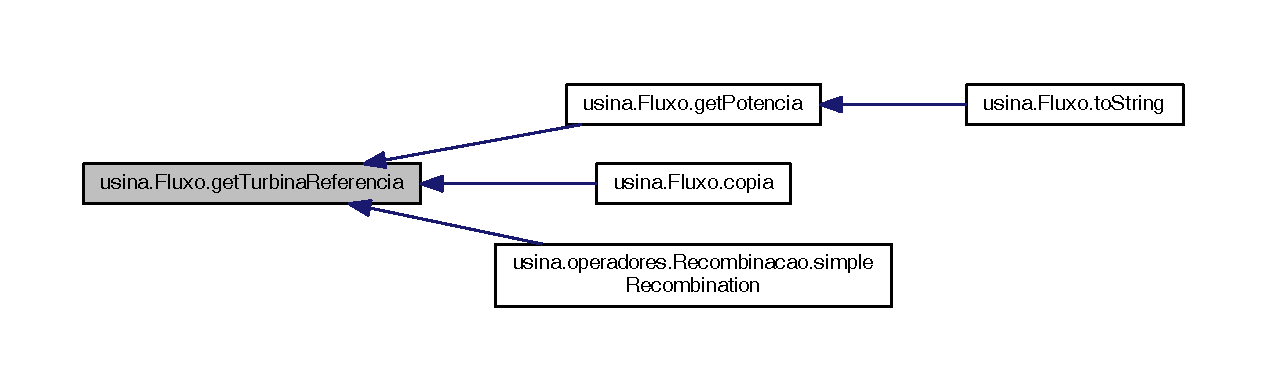
\includegraphics[width=350pt]{classusina_1_1_fluxo_a61cc464f6926c453c51fcded2d57306d_icgraph}
\end{center}
\end{figure}


\hypertarget{classusina_1_1_fluxo_a0634c81d7575ad63274828d8c40a88e5}{\index{usina\-::\-Fluxo@{usina\-::\-Fluxo}!get\-Vazao@{get\-Vazao}}
\index{get\-Vazao@{get\-Vazao}!usina::Fluxo@{usina\-::\-Fluxo}}
\subsubsection[{get\-Vazao}]{\setlength{\rightskip}{0pt plus 5cm}final double usina.\-Fluxo.\-get\-Vazao (
\begin{DoxyParamCaption}
{}
\end{DoxyParamCaption}
)}}\label{classusina_1_1_fluxo_a0634c81d7575ad63274828d8c40a88e5}


Recupera o valor da vazão do fluxo. 

\begin{DoxySince}{Desde}
1.\-0 
\end{DoxySince}
\begin{DoxyReturn}{Retorna}
Valor da vazão. 
\end{DoxyReturn}


Este é o diagrama das funções que utilizam esta função\-:\nopagebreak
\begin{figure}[H]
\begin{center}
\leavevmode
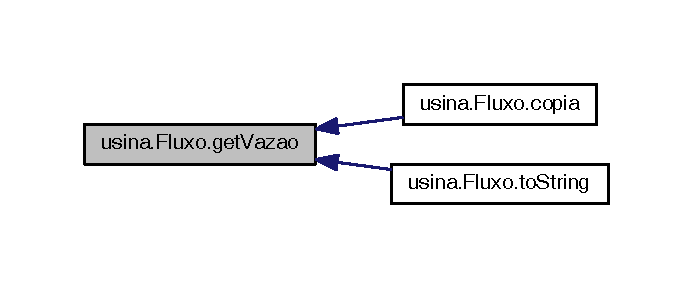
\includegraphics[width=332pt]{classusina_1_1_fluxo_a0634c81d7575ad63274828d8c40a88e5_icgraph}
\end{center}
\end{figure}


\hypertarget{classusina_1_1_fluxo_a1c204862a651d75929b078355b512823}{\index{usina\-::\-Fluxo@{usina\-::\-Fluxo}!set\-Reynolds@{set\-Reynolds}}
\index{set\-Reynolds@{set\-Reynolds}!usina::Fluxo@{usina\-::\-Fluxo}}
\subsubsection[{set\-Reynolds}]{\setlength{\rightskip}{0pt plus 5cm}void usina.\-Fluxo.\-set\-Reynolds (
\begin{DoxyParamCaption}
\item[{Double}]{reynolds}
\end{DoxyParamCaption}
)\hspace{0.3cm}{\ttfamily [private]}}}\label{classusina_1_1_fluxo_a1c204862a651d75929b078355b512823}


Atribui um número de Reynolds ao fluxo. 

\begin{DoxySince}{Desde}
1.\-0 
\end{DoxySince}
\begin{DoxyReturn}{Retorna}
O Coeficiente de Reynolds. 
\end{DoxyReturn}


Este é o diagrama das funções que utilizam esta função\-:\nopagebreak
\begin{figure}[H]
\begin{center}
\leavevmode
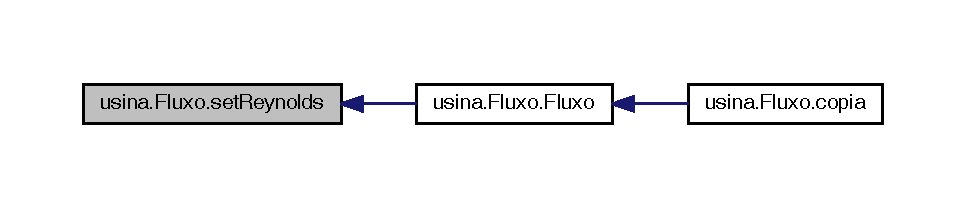
\includegraphics[width=350pt]{classusina_1_1_fluxo_a1c204862a651d75929b078355b512823_icgraph}
\end{center}
\end{figure}


\hypertarget{classusina_1_1_fluxo_a3bb30b3608a7ab915ff332018a18d81f}{\index{usina\-::\-Fluxo@{usina\-::\-Fluxo}!set\-Turbina@{set\-Turbina}}
\index{set\-Turbina@{set\-Turbina}!usina::Fluxo@{usina\-::\-Fluxo}}
\subsubsection[{set\-Turbina}]{\setlength{\rightskip}{0pt plus 5cm}void usina.\-Fluxo.\-set\-Turbina (
\begin{DoxyParamCaption}
\item[{{\bf Turbina}}]{turbina\-Referencia}
\end{DoxyParamCaption}
)\hspace{0.3cm}{\ttfamily [private]}}}\label{classusina_1_1_fluxo_a3bb30b3608a7ab915ff332018a18d81f}


Atribui uma turbina de referência ao fluxo. 

Não deve ser publica, pois o fluxo é semanticamente relacionado a uma turbina. Adicionalmente, essa função não modifica os limites do locus – criados na construção do objeto e não modificáveis. 

\begin{DoxySince}{Desde}
1.\-0 
\end{DoxySince}

\begin{DoxyParams}{Parâmetros}
{\em turbina\-Referencia} & A turbina de referência. \\
\hline
\end{DoxyParams}


Este é o diagrama das funções que utilizam esta função\-:\nopagebreak
\begin{figure}[H]
\begin{center}
\leavevmode
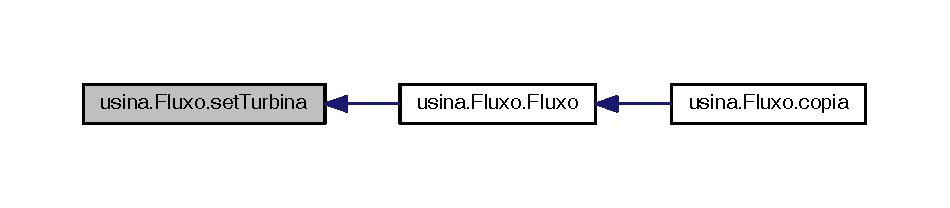
\includegraphics[width=350pt]{classusina_1_1_fluxo_a3bb30b3608a7ab915ff332018a18d81f_icgraph}
\end{center}
\end{figure}


\hypertarget{classusina_1_1_fluxo_af80f13f4ade8128bac424b456ec0836a}{\index{usina\-::\-Fluxo@{usina\-::\-Fluxo}!set\-Vazao@{set\-Vazao}}
\index{set\-Vazao@{set\-Vazao}!usina::Fluxo@{usina\-::\-Fluxo}}
\subsubsection[{set\-Vazao}]{\setlength{\rightskip}{0pt plus 5cm}final void usina.\-Fluxo.\-set\-Vazao (
\begin{DoxyParamCaption}
\item[{Double}]{vazao}
\end{DoxyParamCaption}
)}}\label{classusina_1_1_fluxo_af80f13f4ade8128bac424b456ec0836a}


Atribui um novo valor de vazão ao fluxo. 

\begin{DoxySince}{Desde}
1.\-0 
\end{DoxySince}

\begin{DoxyParams}{Parâmetros}
{\em vazao} & Nova vazão.\\
\hline
\end{DoxyParams}

\begin{DoxyExceptions}{Exceções}
{\em Illegal\-Argument\-Exception} & 
\begin{DoxyItemize}
\item Se o valor estiver fora dos limites -\/ impostos pela turbina.  
\end{DoxyItemize}\\
\hline
\end{DoxyExceptions}
\begin{DoxySeeAlso}{Veja também}
Locus\-Real\-::set\-Locus(java.\-lang.\-Double) 
\end{DoxySeeAlso}


Este é o diagrama das funções que utilizam esta função\-:\nopagebreak
\begin{figure}[H]
\begin{center}
\leavevmode
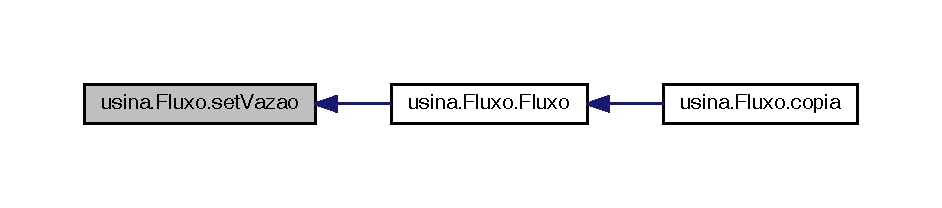
\includegraphics[width=350pt]{classusina_1_1_fluxo_af80f13f4ade8128bac424b456ec0836a_icgraph}
\end{center}
\end{figure}


\hypertarget{classusina_1_1_fluxo_aa7c07414a1af3c807312950fa5019591}{\index{usina\-::\-Fluxo@{usina\-::\-Fluxo}!to\-String@{to\-String}}
\index{to\-String@{to\-String}!usina::Fluxo@{usina\-::\-Fluxo}}
\subsubsection[{to\-String}]{\setlength{\rightskip}{0pt plus 5cm}String usina.\-Fluxo.\-to\-String (
\begin{DoxyParamCaption}
{}
\end{DoxyParamCaption}
)}}\label{classusina_1_1_fluxo_aa7c07414a1af3c807312950fa5019591}


Este é o diagrama das funções utilizadas por esta função\-:
\nopagebreak
\begin{figure}[H]
\begin{center}
\leavevmode
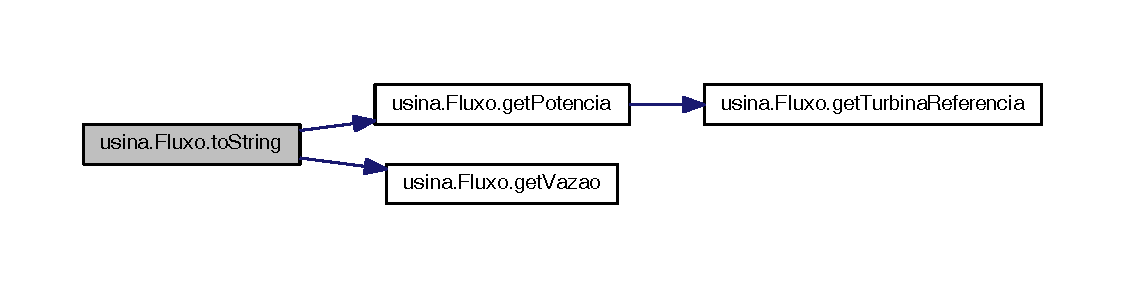
\includegraphics[width=350pt]{classusina_1_1_fluxo_aa7c07414a1af3c807312950fa5019591_cgraph}
\end{center}
\end{figure}




\subsection{Atributos}
\hypertarget{classusina_1_1_fluxo_a185fed046eefce4fa8f8bb10fde8296d}{\index{usina\-::\-Fluxo@{usina\-::\-Fluxo}!reynolds@{reynolds}}
\index{reynolds@{reynolds}!usina::Fluxo@{usina\-::\-Fluxo}}
\subsubsection[{reynolds}]{\setlength{\rightskip}{0pt plus 5cm}Double usina.\-Fluxo.\-reynolds\hspace{0.3cm}{\ttfamily [private]}}}\label{classusina_1_1_fluxo_a185fed046eefce4fa8f8bb10fde8296d}
\hypertarget{classusina_1_1_fluxo_ad85aeeb220a6c87764d29ce36bb8cc26}{\index{usina\-::\-Fluxo@{usina\-::\-Fluxo}!R\-E\-Y\-N\-O\-L\-D\-S\-\_\-\-P\-A\-D\-R\-A\-O@{R\-E\-Y\-N\-O\-L\-D\-S\-\_\-\-P\-A\-D\-R\-A\-O}}
\index{R\-E\-Y\-N\-O\-L\-D\-S\-\_\-\-P\-A\-D\-R\-A\-O@{R\-E\-Y\-N\-O\-L\-D\-S\-\_\-\-P\-A\-D\-R\-A\-O}!usina::Fluxo@{usina\-::\-Fluxo}}
\subsubsection[{R\-E\-Y\-N\-O\-L\-D\-S\-\_\-\-P\-A\-D\-R\-A\-O}]{\setlength{\rightskip}{0pt plus 5cm}final Double usina.\-Fluxo.\-R\-E\-Y\-N\-O\-L\-D\-S\-\_\-\-P\-A\-D\-R\-A\-O = 70000.\-0\hspace{0.3cm}{\ttfamily [static]}}}\label{classusina_1_1_fluxo_ad85aeeb220a6c87764d29ce36bb8cc26}
\hypertarget{classusina_1_1_fluxo_aee04932f02b1bfad1bf79cc80a1df203}{\index{usina\-::\-Fluxo@{usina\-::\-Fluxo}!turbina\-Referencia@{turbina\-Referencia}}
\index{turbina\-Referencia@{turbina\-Referencia}!usina::Fluxo@{usina\-::\-Fluxo}}
\subsubsection[{turbina\-Referencia}]{\setlength{\rightskip}{0pt plus 5cm}{\bf Turbina} usina.\-Fluxo.\-turbina\-Referencia\hspace{0.3cm}{\ttfamily [private]}}}\label{classusina_1_1_fluxo_aee04932f02b1bfad1bf79cc80a1df203}


A documentação para esta classe foi gerada a partir do seguinte arquivo\-:\begin{DoxyCompactItemize}
\item 
C\-:/\-Users/\-Victor/workplace/\-Net\-Beans\-Projects/tcc/src/usina/\hyperlink{_fluxo_8java}{Fluxo.\-java}\end{DoxyCompactItemize}

\hypertarget{classusina_1_1operadores_1_1_geracao}{\section{Referência da Classe usina.\-operadores.\-Geracao}
\label{classusina_1_1operadores_1_1_geracao}\index{usina.\-operadores.\-Geracao@{usina.\-operadores.\-Geracao}}
}


Diagrama de Hierarquia para usina.\-operadores.\-Geracao\-:
\nopagebreak
\begin{figure}[H]
\begin{center}
\leavevmode
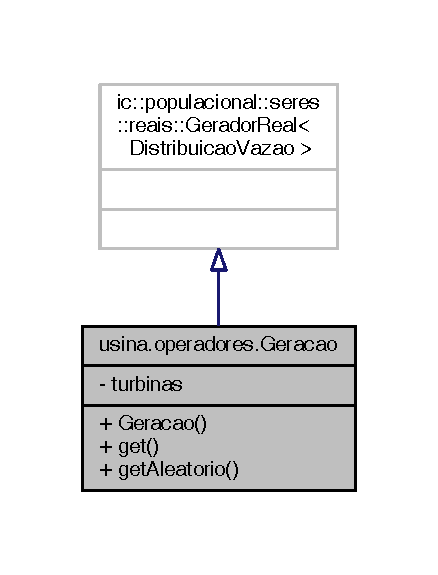
\includegraphics[width=210pt]{classusina_1_1operadores_1_1_geracao__inherit__graph}
\end{center}
\end{figure}


Diagrama de colaboração para usina.\-operadores.\-Geracao\-:
\nopagebreak
\begin{figure}[H]
\begin{center}
\leavevmode
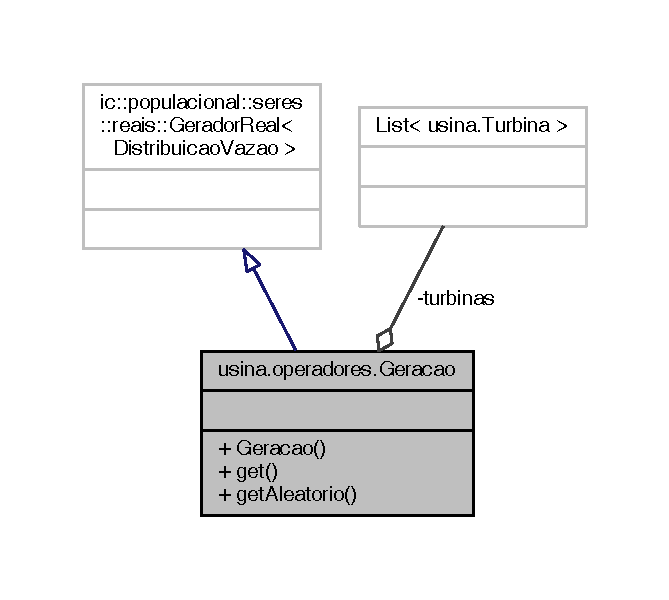
\includegraphics[width=321pt]{classusina_1_1operadores_1_1_geracao__coll__graph}
\end{center}
\end{figure}
\subsection*{Métodos Públicos}
\begin{DoxyCompactItemize}
\item 
\hyperlink{classusina_1_1operadores_1_1_geracao_ab334f542469af41831192f8ca44379ba}{Geracao} (List$<$ \hyperlink{classusina_1_1_turbina}{Turbina} $>$ \hyperlink{classusina_1_1operadores_1_1_geracao_af3e8001df85b6894c6eeeec336851473}{turbinas})
\begin{DoxyCompactList}\small\item\em Construtor. \end{DoxyCompactList}\item 
\hyperlink{classusina_1_1_distribuicao_vazao}{Distribuicao\-Vazao} \hyperlink{classusina_1_1operadores_1_1_geracao_a1fa1d2616b22de7bc1f8f35ac51df288}{get} ()
\item 
\hyperlink{classusina_1_1_distribuicao_vazao}{Distribuicao\-Vazao} \hyperlink{classusina_1_1operadores_1_1_geracao_a97d1ce85305dd4bbfcef3113a8578b7e}{get\-Aleatorio} ()
\end{DoxyCompactItemize}
\subsection*{Atributos Privados}
\begin{DoxyCompactItemize}
\item 
final List$<$ \hyperlink{classusina_1_1_turbina}{Turbina} $>$ \hyperlink{classusina_1_1operadores_1_1_geracao_af3e8001df85b6894c6eeeec336851473}{turbinas}
\end{DoxyCompactItemize}


\subsection{Descrição Detalhada}
\begin{DoxyAuthor}{Autor}
Victor de Lima Soares 
\end{DoxyAuthor}


\subsection{Construtores \& Destrutores}
\hypertarget{classusina_1_1operadores_1_1_geracao_ab334f542469af41831192f8ca44379ba}{\index{usina\-::operadores\-::\-Geracao@{usina\-::operadores\-::\-Geracao}!Geracao@{Geracao}}
\index{Geracao@{Geracao}!usina::operadores::Geracao@{usina\-::operadores\-::\-Geracao}}
\subsubsection[{Geracao}]{\setlength{\rightskip}{0pt plus 5cm}usina.\-operadores.\-Geracao.\-Geracao (
\begin{DoxyParamCaption}
\item[{List$<$ {\bf Turbina} $>$}]{turbinas}
\end{DoxyParamCaption}
)}}\label{classusina_1_1operadores_1_1_geracao_ab334f542469af41831192f8ca44379ba}


Construtor. 


\begin{DoxyParams}{Parâmetros}
{\em turbinas} & \\
\hline
\end{DoxyParams}

\begin{DoxyExceptions}{Exceções}
{\em Null\-Pointer\-Exception} & 
\begin{DoxyItemize}
\item Se a lista de turbinas for uma referência nula. 
\end{DoxyItemize}\\
\hline
\end{DoxyExceptions}


\subsection{Métodos}
\hypertarget{classusina_1_1operadores_1_1_geracao_a1fa1d2616b22de7bc1f8f35ac51df288}{\index{usina\-::operadores\-::\-Geracao@{usina\-::operadores\-::\-Geracao}!get@{get}}
\index{get@{get}!usina::operadores::Geracao@{usina\-::operadores\-::\-Geracao}}
\subsubsection[{get}]{\setlength{\rightskip}{0pt plus 5cm}{\bf Distribuicao\-Vazao} usina.\-operadores.\-Geracao.\-get (
\begin{DoxyParamCaption}
{}
\end{DoxyParamCaption}
)}}\label{classusina_1_1operadores_1_1_geracao_a1fa1d2616b22de7bc1f8f35ac51df288}
\hypertarget{classusina_1_1operadores_1_1_geracao_a97d1ce85305dd4bbfcef3113a8578b7e}{\index{usina\-::operadores\-::\-Geracao@{usina\-::operadores\-::\-Geracao}!get\-Aleatorio@{get\-Aleatorio}}
\index{get\-Aleatorio@{get\-Aleatorio}!usina::operadores::Geracao@{usina\-::operadores\-::\-Geracao}}
\subsubsection[{get\-Aleatorio}]{\setlength{\rightskip}{0pt plus 5cm}{\bf Distribuicao\-Vazao} usina.\-operadores.\-Geracao.\-get\-Aleatorio (
\begin{DoxyParamCaption}
{}
\end{DoxyParamCaption}
)}}\label{classusina_1_1operadores_1_1_geracao_a97d1ce85305dd4bbfcef3113a8578b7e}


\subsection{Atributos}
\hypertarget{classusina_1_1operadores_1_1_geracao_af3e8001df85b6894c6eeeec336851473}{\index{usina\-::operadores\-::\-Geracao@{usina\-::operadores\-::\-Geracao}!turbinas@{turbinas}}
\index{turbinas@{turbinas}!usina::operadores::Geracao@{usina\-::operadores\-::\-Geracao}}
\subsubsection[{turbinas}]{\setlength{\rightskip}{0pt plus 5cm}final List$<${\bf Turbina}$>$ usina.\-operadores.\-Geracao.\-turbinas\hspace{0.3cm}{\ttfamily [private]}}}\label{classusina_1_1operadores_1_1_geracao_af3e8001df85b6894c6eeeec336851473}


A documentação para esta classe foi gerada a partir do seguinte arquivo\-:\begin{DoxyCompactItemize}
\item 
C\-:/\-Users/\-Victor/workplace/\-Net\-Beans\-Projects/tcc/src/usina/operadores/\hyperlink{_geracao_8java}{Geracao.\-java}\end{DoxyCompactItemize}

\hypertarget{classusina_1_1operadores_1_1_mutacao}{\section{Referência da Classe usina.\-operadores.\-Mutacao}
\label{classusina_1_1operadores_1_1_mutacao}\index{usina.\-operadores.\-Mutacao@{usina.\-operadores.\-Mutacao}}
}


Diagrama de Hierarquia para usina.\-operadores.\-Mutacao\-:\nopagebreak
\begin{figure}[H]
\begin{center}
\leavevmode
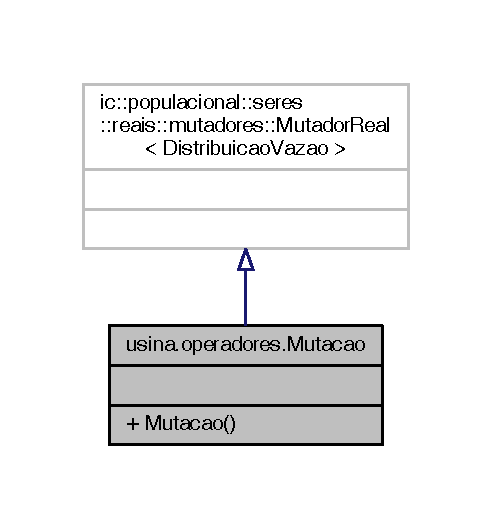
\includegraphics[width=236pt]{classusina_1_1operadores_1_1_mutacao__inherit__graph}
\end{center}
\end{figure}


Diagrama de colaboração para usina.\-operadores.\-Mutacao\-:\nopagebreak
\begin{figure}[H]
\begin{center}
\leavevmode
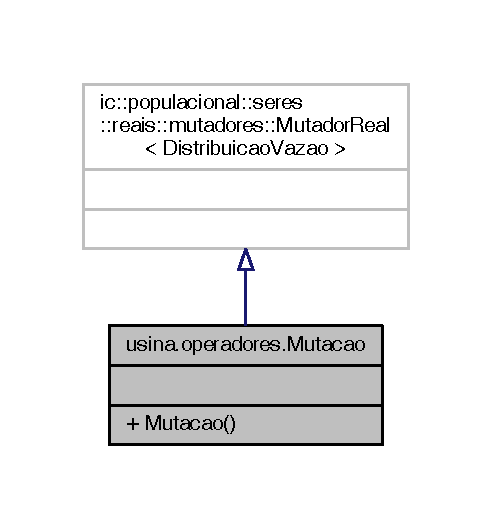
\includegraphics[width=236pt]{classusina_1_1operadores_1_1_mutacao__coll__graph}
\end{center}
\end{figure}
\subsection*{Métodos Públicos}
\begin{DoxyCompactItemize}
\item 
\hyperlink{classusina_1_1operadores_1_1_mutacao_a77ff4d6902397c6b788cfc90342a1030}{Mutacao} (double probabilidade\-De\-Mutacao)
\end{DoxyCompactItemize}


\subsection{Descrição Detalhada}
\begin{DoxyAuthor}{Autor}
Victor de Lima Soares 
\end{DoxyAuthor}


\subsection{Construtores \& Destrutores}
\hypertarget{classusina_1_1operadores_1_1_mutacao_a77ff4d6902397c6b788cfc90342a1030}{\index{usina\-::operadores\-::\-Mutacao@{usina\-::operadores\-::\-Mutacao}!Mutacao@{Mutacao}}
\index{Mutacao@{Mutacao}!usina::operadores::Mutacao@{usina\-::operadores\-::\-Mutacao}}
\subsubsection[{Mutacao}]{\setlength{\rightskip}{0pt plus 5cm}usina.\-operadores.\-Mutacao.\-Mutacao (
\begin{DoxyParamCaption}
\item[{double}]{probabilidade\-De\-Mutacao}
\end{DoxyParamCaption}
)}}\label{classusina_1_1operadores_1_1_mutacao_a77ff4d6902397c6b788cfc90342a1030}


A documentação para esta classe foi gerada a partir do seguinte arquivo\-:\begin{DoxyCompactItemize}
\item 
C\-:/\-Users/\-Victor/workplace/\-Net\-Beans\-Projects/tcc/src/usina/operadores/\hyperlink{_mutacao_8java}{Mutacao.\-java}\end{DoxyCompactItemize}

\hypertarget{classusina_1_1_populacao_de_distribuicoes}{\section{Referência da Classe usina.\-Populacao\-De\-Distribuicoes}
\label{classusina_1_1_populacao_de_distribuicoes}\index{usina.\-Populacao\-De\-Distribuicoes@{usina.\-Populacao\-De\-Distribuicoes}}
}


População de distribuições.  




Diagrama de Hierarquia para usina.\-Populacao\-De\-Distribuicoes\-:\nopagebreak
\begin{figure}[H]
\begin{center}
\leavevmode
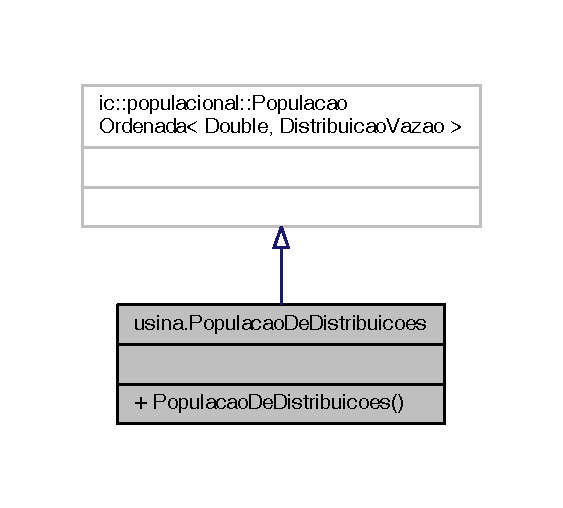
\includegraphics[width=270pt]{classusina_1_1_populacao_de_distribuicoes__inherit__graph}
\end{center}
\end{figure}


Diagrama de colaboração para usina.\-Populacao\-De\-Distribuicoes\-:\nopagebreak
\begin{figure}[H]
\begin{center}
\leavevmode
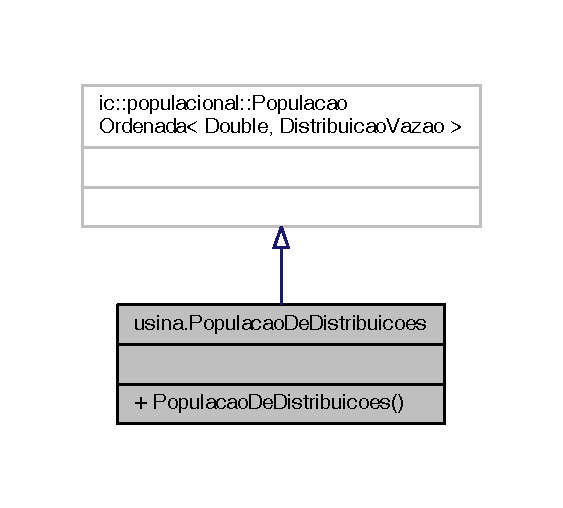
\includegraphics[width=270pt]{classusina_1_1_populacao_de_distribuicoes__coll__graph}
\end{center}
\end{figure}
\subsection*{Métodos Públicos}
\begin{DoxyCompactItemize}
\item 
\hyperlink{classusina_1_1_populacao_de_distribuicoes_aef0a6e6048fdefa0be86d4ba7064e13d}{Populacao\-De\-Distribuicoes} (\hyperlink{classusina_1_1_usina}{Usina} ambiente, Integer max\-Individuos)
\end{DoxyCompactItemize}


\subsection{Descrição Detalhada}
População de distribuições. 

Essa classe representa um coletivo para distribuições de vazão, fornecendo uma interface para manipulação do conjunto por algoritmos evolucionários. 

\begin{DoxyAuthor}{Autor}
Victor de Lima Soares
\end{DoxyAuthor}
\begin{DoxyVersion}{Versão}
1.\-0 
\end{DoxyVersion}
\begin{DoxySeeAlso}{Veja também}

\end{DoxySeeAlso}


\subsection{Construtores \& Destrutores}
\hypertarget{classusina_1_1_populacao_de_distribuicoes_aef0a6e6048fdefa0be86d4ba7064e13d}{\index{usina\-::\-Populacao\-De\-Distribuicoes@{usina\-::\-Populacao\-De\-Distribuicoes}!Populacao\-De\-Distribuicoes@{Populacao\-De\-Distribuicoes}}
\index{Populacao\-De\-Distribuicoes@{Populacao\-De\-Distribuicoes}!usina::PopulacaoDeDistribuicoes@{usina\-::\-Populacao\-De\-Distribuicoes}}
\subsubsection[{Populacao\-De\-Distribuicoes}]{\setlength{\rightskip}{0pt plus 5cm}usina.\-Populacao\-De\-Distribuicoes.\-Populacao\-De\-Distribuicoes (
\begin{DoxyParamCaption}
\item[{{\bf Usina}}]{ambiente, }
\item[{Integer}]{max\-Individuos}
\end{DoxyParamCaption}
)}}\label{classusina_1_1_populacao_de_distribuicoes_aef0a6e6048fdefa0be86d4ba7064e13d}


A documentação para esta classe foi gerada a partir do seguinte arquivo\-:\begin{DoxyCompactItemize}
\item 
C\-:/\-Users/\-Victor/workplace/\-Net\-Beans\-Projects/tcc/src/usina/\hyperlink{_populacao_de_distribuicoes_8java}{Populacao\-De\-Distribuicoes.\-java}\end{DoxyCompactItemize}

\hypertarget{classusina_1_1operadores_1_1_recombinacao}{\section{Referência da Classe usina.\-operadores.\-Recombinacao}
\label{classusina_1_1operadores_1_1_recombinacao}\index{usina.\-operadores.\-Recombinacao@{usina.\-operadores.\-Recombinacao}}
}


Diagrama de Hierarquia para usina.\-operadores.\-Recombinacao\-:
\nopagebreak
\begin{figure}[H]
\begin{center}
\leavevmode
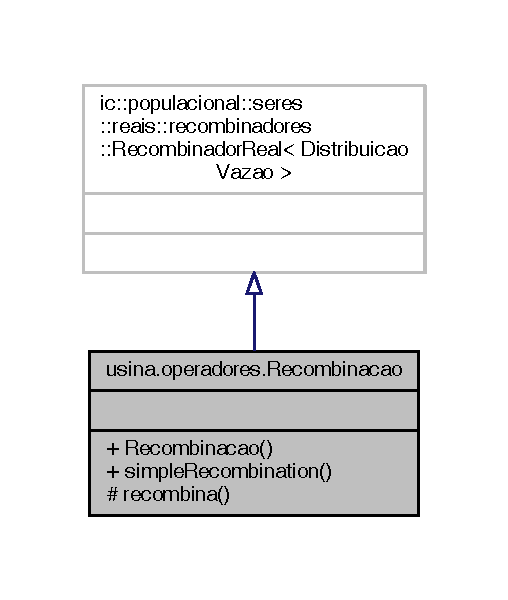
\includegraphics[width=244pt]{classusina_1_1operadores_1_1_recombinacao__inherit__graph}
\end{center}
\end{figure}


Diagrama de colaboração para usina.\-operadores.\-Recombinacao\-:
\nopagebreak
\begin{figure}[H]
\begin{center}
\leavevmode
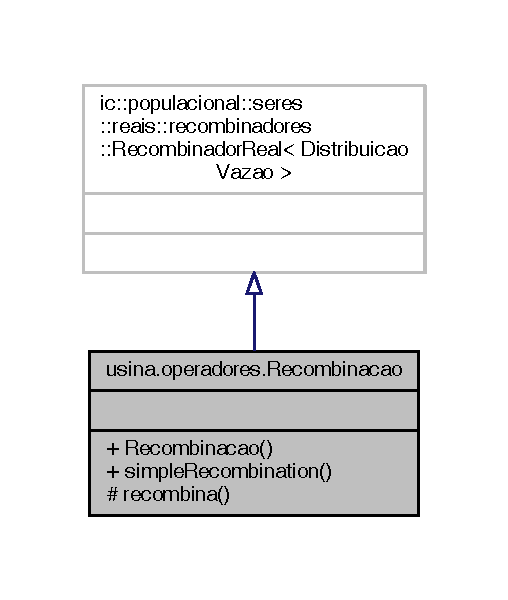
\includegraphics[width=244pt]{classusina_1_1operadores_1_1_recombinacao__coll__graph}
\end{center}
\end{figure}
\subsection*{Métodos Públicos}
\begin{DoxyCompactItemize}
\item 
\hyperlink{classusina_1_1operadores_1_1_recombinacao_aa0b470f925dd33c385f221159ef5a553}{Recombinacao} (Gerador$<$ \hyperlink{classusina_1_1_distribuicao_vazao}{Distribuicao\-Vazao} $>$ gerador, Double probabilidade\-De\-Recombinacao)
\item 
List$<$ \hyperlink{classusina_1_1_distribuicao_vazao}{Distribuicao\-Vazao} $>$ \hyperlink{classusina_1_1operadores_1_1_recombinacao_aec7a06aa6a7de39a4407fd230dae656a}{simple\-Recombination} (int k, double alfa, \hyperlink{classusina_1_1_distribuicao_vazao}{Distribuicao\-Vazao} par1, \hyperlink{classusina_1_1_distribuicao_vazao}{Distribuicao\-Vazao} par2)
\end{DoxyCompactItemize}
\subsection*{Métodos Protegidos}
\begin{DoxyCompactItemize}
\item 
List$<$ \hyperlink{classusina_1_1_distribuicao_vazao}{Distribuicao\-Vazao} $>$ \hyperlink{classusina_1_1operadores_1_1_recombinacao_a814b21721f4b2ce29e8838fff9ce3f5e}{recombina} (List$<$ \hyperlink{classusina_1_1_distribuicao_vazao}{Distribuicao\-Vazao} $>$ pares)
\end{DoxyCompactItemize}


\subsection{Descrição Detalhada}
\begin{DoxyAuthor}{Autor}
Victor de Lima Soares 
\end{DoxyAuthor}


\subsection{Construtores \& Destrutores}
\hypertarget{classusina_1_1operadores_1_1_recombinacao_aa0b470f925dd33c385f221159ef5a553}{\index{usina\-::operadores\-::\-Recombinacao@{usina\-::operadores\-::\-Recombinacao}!Recombinacao@{Recombinacao}}
\index{Recombinacao@{Recombinacao}!usina::operadores::Recombinacao@{usina\-::operadores\-::\-Recombinacao}}
\subsubsection[{Recombinacao}]{\setlength{\rightskip}{0pt plus 5cm}usina.\-operadores.\-Recombinacao.\-Recombinacao (
\begin{DoxyParamCaption}
\item[{Gerador$<$ {\bf Distribuicao\-Vazao} $>$}]{gerador, }
\item[{Double}]{probabilidade\-De\-Recombinacao}
\end{DoxyParamCaption}
)}}\label{classusina_1_1operadores_1_1_recombinacao_aa0b470f925dd33c385f221159ef5a553}


\subsection{Métodos}
\hypertarget{classusina_1_1operadores_1_1_recombinacao_a814b21721f4b2ce29e8838fff9ce3f5e}{\index{usina\-::operadores\-::\-Recombinacao@{usina\-::operadores\-::\-Recombinacao}!recombina@{recombina}}
\index{recombina@{recombina}!usina::operadores::Recombinacao@{usina\-::operadores\-::\-Recombinacao}}
\subsubsection[{recombina}]{\setlength{\rightskip}{0pt plus 5cm}List$<${\bf Distribuicao\-Vazao}$>$ usina.\-operadores.\-Recombinacao.\-recombina (
\begin{DoxyParamCaption}
\item[{List$<$ {\bf Distribuicao\-Vazao} $>$}]{pares}
\end{DoxyParamCaption}
)\hspace{0.3cm}{\ttfamily [protected]}}}\label{classusina_1_1operadores_1_1_recombinacao_a814b21721f4b2ce29e8838fff9ce3f5e}
\hypertarget{classusina_1_1operadores_1_1_recombinacao_aec7a06aa6a7de39a4407fd230dae656a}{\index{usina\-::operadores\-::\-Recombinacao@{usina\-::operadores\-::\-Recombinacao}!simple\-Recombination@{simple\-Recombination}}
\index{simple\-Recombination@{simple\-Recombination}!usina::operadores::Recombinacao@{usina\-::operadores\-::\-Recombinacao}}
\subsubsection[{simple\-Recombination}]{\setlength{\rightskip}{0pt plus 5cm}List$<${\bf Distribuicao\-Vazao}$>$ usina.\-operadores.\-Recombinacao.\-simple\-Recombination (
\begin{DoxyParamCaption}
\item[{int}]{k, }
\item[{double}]{alfa, }
\item[{{\bf Distribuicao\-Vazao}}]{par1, }
\item[{{\bf Distribuicao\-Vazao}}]{par2}
\end{DoxyParamCaption}
)}}\label{classusina_1_1operadores_1_1_recombinacao_aec7a06aa6a7de39a4407fd230dae656a}


Este é o diagrama das funções utilizadas por esta função\-:
\nopagebreak
\begin{figure}[H]
\begin{center}
\leavevmode
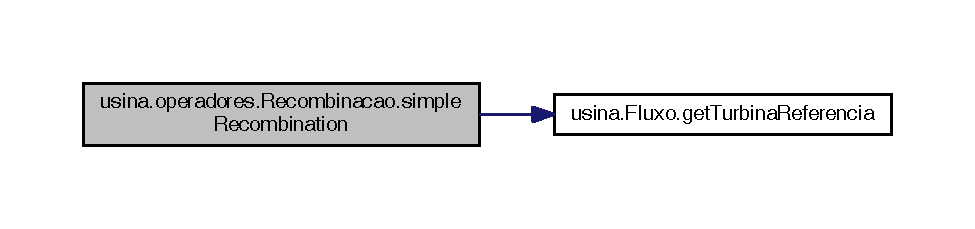
\includegraphics[width=350pt]{classusina_1_1operadores_1_1_recombinacao_aec7a06aa6a7de39a4407fd230dae656a_cgraph}
\end{center}
\end{figure}




A documentação para esta classe foi gerada a partir do seguinte arquivo\-:\begin{DoxyCompactItemize}
\item 
C\-:/\-Users/\-Victor/workplace/\-Net\-Beans\-Projects/tcc/src/usina/operadores/\hyperlink{_recombinacao_8java}{Recombinacao.\-java}\end{DoxyCompactItemize}

\hypertarget{classusina_1_1operadores_1_1_selecao}{\section{Referência da Classe usina.\-operadores.\-Selecao}
\label{classusina_1_1operadores_1_1_selecao}\index{usina.\-operadores.\-Selecao@{usina.\-operadores.\-Selecao}}
}


Diagrama de Hierarquia para usina.\-operadores.\-Selecao\-:\nopagebreak
\begin{figure}[H]
\begin{center}
\leavevmode
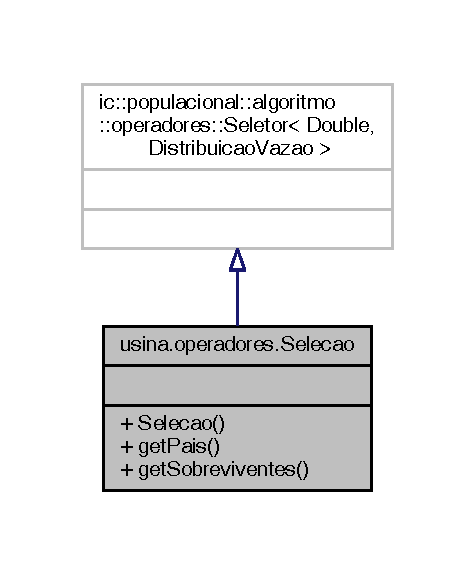
\includegraphics[width=228pt]{classusina_1_1operadores_1_1_selecao__inherit__graph}
\end{center}
\end{figure}


Diagrama de colaboração para usina.\-operadores.\-Selecao\-:\nopagebreak
\begin{figure}[H]
\begin{center}
\leavevmode
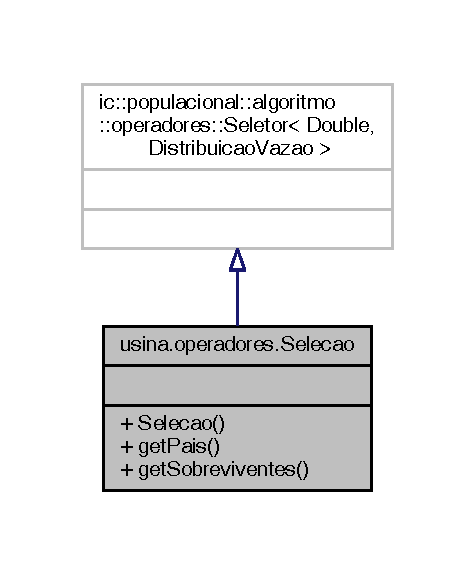
\includegraphics[width=228pt]{classusina_1_1operadores_1_1_selecao__coll__graph}
\end{center}
\end{figure}
\subsection*{Métodos Públicos}
\begin{DoxyCompactItemize}
\item 
\hyperlink{classusina_1_1operadores_1_1_selecao_affd73c5918fbe7de9217f90c17a26468}{Selecao} (Ambiente ambiente, Populacao populacao)
\item 
List$<$ \hyperlink{classusina_1_1_distribuicao_vazao}{Distribuicao\-Vazao} $>$ \hyperlink{classusina_1_1operadores_1_1_selecao_abe8838b51ba7038b6bb59052c8ca77ac}{get\-Pais} ()
\item 
List$<$ \hyperlink{classusina_1_1_distribuicao_vazao}{Distribuicao\-Vazao} $>$ \hyperlink{classusina_1_1operadores_1_1_selecao_abf5eab42a3c05ff5c0550f59297a50d3}{get\-Sobreviventes} ()
\end{DoxyCompactItemize}


\subsection{Descrição Detalhada}
\begin{DoxyAuthor}{Autor}
Victor de Lima Soares 
\end{DoxyAuthor}


\subsection{Construtores \& Destrutores}
\hypertarget{classusina_1_1operadores_1_1_selecao_affd73c5918fbe7de9217f90c17a26468}{\index{usina\-::operadores\-::\-Selecao@{usina\-::operadores\-::\-Selecao}!Selecao@{Selecao}}
\index{Selecao@{Selecao}!usina::operadores::Selecao@{usina\-::operadores\-::\-Selecao}}
\subsubsection[{Selecao}]{\setlength{\rightskip}{0pt plus 5cm}usina.\-operadores.\-Selecao.\-Selecao (
\begin{DoxyParamCaption}
\item[{Ambiente}]{ambiente, }
\item[{Populacao}]{populacao}
\end{DoxyParamCaption}
)}}\label{classusina_1_1operadores_1_1_selecao_affd73c5918fbe7de9217f90c17a26468}


\subsection{Métodos}
\hypertarget{classusina_1_1operadores_1_1_selecao_abe8838b51ba7038b6bb59052c8ca77ac}{\index{usina\-::operadores\-::\-Selecao@{usina\-::operadores\-::\-Selecao}!get\-Pais@{get\-Pais}}
\index{get\-Pais@{get\-Pais}!usina::operadores::Selecao@{usina\-::operadores\-::\-Selecao}}
\subsubsection[{get\-Pais}]{\setlength{\rightskip}{0pt plus 5cm}List$<${\bf Distribuicao\-Vazao}$>$ usina.\-operadores.\-Selecao.\-get\-Pais (
\begin{DoxyParamCaption}
{}
\end{DoxyParamCaption}
)}}\label{classusina_1_1operadores_1_1_selecao_abe8838b51ba7038b6bb59052c8ca77ac}
\hypertarget{classusina_1_1operadores_1_1_selecao_abf5eab42a3c05ff5c0550f59297a50d3}{\index{usina\-::operadores\-::\-Selecao@{usina\-::operadores\-::\-Selecao}!get\-Sobreviventes@{get\-Sobreviventes}}
\index{get\-Sobreviventes@{get\-Sobreviventes}!usina::operadores::Selecao@{usina\-::operadores\-::\-Selecao}}
\subsubsection[{get\-Sobreviventes}]{\setlength{\rightskip}{0pt plus 5cm}List$<${\bf Distribuicao\-Vazao}$>$ usina.\-operadores.\-Selecao.\-get\-Sobreviventes (
\begin{DoxyParamCaption}
{}
\end{DoxyParamCaption}
)}}\label{classusina_1_1operadores_1_1_selecao_abf5eab42a3c05ff5c0550f59297a50d3}


A documentação para esta classe foi gerada a partir do seguinte arquivo\-:\begin{DoxyCompactItemize}
\item 
C\-:/\-Users/\-Victor/workplace/\-Net\-Beans\-Projects/tcc/src/usina/operadores/\hyperlink{_selecao_8java}{Selecao.\-java}\end{DoxyCompactItemize}

\hypertarget{classtcc_1_1_simulacao}{\section{Referência da Classe tcc.\-Simulacao}
\label{classtcc_1_1_simulacao}\index{tcc.\-Simulacao@{tcc.\-Simulacao}}
}


Diagrama de colaboração para tcc.\-Simulacao\-:
\nopagebreak
\begin{figure}[H]
\begin{center}
\leavevmode
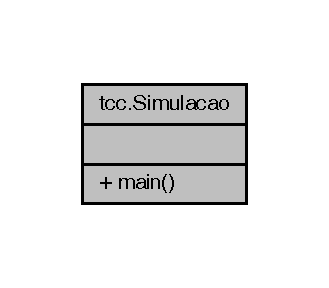
\includegraphics[width=158pt]{classtcc_1_1_simulacao__coll__graph}
\end{center}
\end{figure}
\subsection*{Métodos Públicos Estáticos}
\begin{DoxyCompactItemize}
\item 
static void \hyperlink{classtcc_1_1_simulacao_a7bd0e9c7094268fe3262733ac599f17b}{main} (String\mbox{[}$\,$\mbox{]} args)
\end{DoxyCompactItemize}


\subsection{Descrição Detalhada}
\begin{DoxyAuthor}{Autor}
Victor de Lima Soares 
\end{DoxyAuthor}
\begin{DoxyVersion}{Versão}
1.\-0 
\end{DoxyVersion}


\subsection{Métodos}
\hypertarget{classtcc_1_1_simulacao_a7bd0e9c7094268fe3262733ac599f17b}{\index{tcc\-::\-Simulacao@{tcc\-::\-Simulacao}!main@{main}}
\index{main@{main}!tcc::Simulacao@{tcc\-::\-Simulacao}}
\subsubsection[{main}]{\setlength{\rightskip}{0pt plus 5cm}static void tcc.\-Simulacao.\-main (
\begin{DoxyParamCaption}
\item[{String\mbox{[}$\,$\mbox{]}}]{args}
\end{DoxyParamCaption}
)\hspace{0.3cm}{\ttfamily [static]}}}\label{classtcc_1_1_simulacao_a7bd0e9c7094268fe3262733ac599f17b}


Este é o diagrama das funções utilizadas por esta função\-:\nopagebreak
\begin{figure}[H]
\begin{center}
\leavevmode
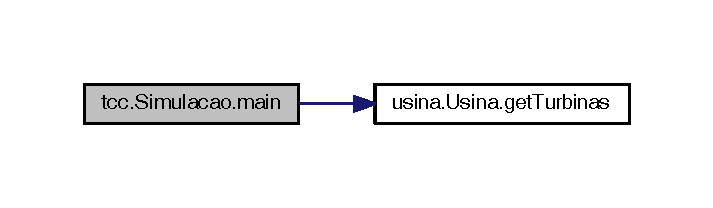
\includegraphics[width=342pt]{classtcc_1_1_simulacao_a7bd0e9c7094268fe3262733ac599f17b_cgraph}
\end{center}
\end{figure}




A documentação para esta classe foi gerada a partir do seguinte arquivo\-:\begin{DoxyCompactItemize}
\item 
C\-:/\-Users/\-Victor/workplace/\-Net\-Beans\-Projects/tcc/src/tcc/\hyperlink{_simulacao_8java}{Simulacao.\-java}\end{DoxyCompactItemize}

\hypertarget{classusina_1_1_d_a_o_1_1turbina_1_1_tubina_d_a_o_factory}{\section{Referência da Classe usina.\-D\-A\-O.\-turbina.\-Tubina\-D\-A\-O\-Factory}
\label{classusina_1_1_d_a_o_1_1turbina_1_1_tubina_d_a_o_factory}\index{usina.\-D\-A\-O.\-turbina.\-Tubina\-D\-A\-O\-Factory@{usina.\-D\-A\-O.\-turbina.\-Tubina\-D\-A\-O\-Factory}}
}


Diagrama de colaboração para usina.\-D\-A\-O.\-turbina.\-Tubina\-D\-A\-O\-Factory\-:\nopagebreak
\begin{figure}[H]
\begin{center}
\leavevmode
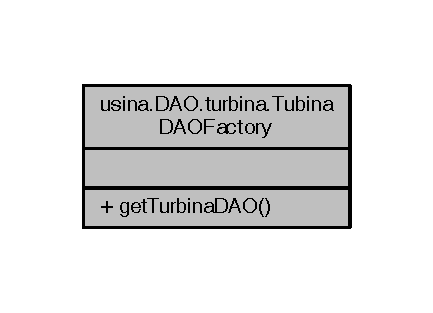
\includegraphics[width=208pt]{classusina_1_1_d_a_o_1_1turbina_1_1_tubina_d_a_o_factory__coll__graph}
\end{center}
\end{figure}
\subsection*{Componentes}
\begin{DoxyCompactItemize}
\item 
enum \hyperlink{enumusina_1_1_d_a_o_1_1turbina_1_1_tubina_d_a_o_factory_1_1_d_a_o_types}{D\-A\-O\-Types}
\end{DoxyCompactItemize}
\subsection*{Métodos Públicos Estáticos}
\begin{DoxyCompactItemize}
\item 
static \hyperlink{interfaceusina_1_1_d_a_o_1_1turbina_1_1_turbina_d_a_o}{Turbina\-D\-A\-O} \hyperlink{classusina_1_1_d_a_o_1_1turbina_1_1_tubina_d_a_o_factory_ad059e78604c0cad0e811022fce6609bc}{get\-Turbina\-D\-A\-O} (\hyperlink{enumusina_1_1_d_a_o_1_1turbina_1_1_tubina_d_a_o_factory_1_1_d_a_o_types}{D\-A\-O\-Types} source\-Type)
\end{DoxyCompactItemize}


\subsection{Descrição Detalhada}
\begin{DoxyAuthor}{Autor}
Victor Soares 
\end{DoxyAuthor}
\begin{DoxyVersion}{Versão}
1.\-0
\end{DoxyVersion}
\begin{DoxyRefDesc}{Descontinuado(a)}
\item[\hyperlink{deprecated__deprecated000001}{Descontinuado(a)}]\end{DoxyRefDesc}


\subsection{Métodos}
\hypertarget{classusina_1_1_d_a_o_1_1turbina_1_1_tubina_d_a_o_factory_ad059e78604c0cad0e811022fce6609bc}{\index{usina\-::\-D\-A\-O\-::turbina\-::\-Tubina\-D\-A\-O\-Factory@{usina\-::\-D\-A\-O\-::turbina\-::\-Tubina\-D\-A\-O\-Factory}!get\-Turbina\-D\-A\-O@{get\-Turbina\-D\-A\-O}}
\index{get\-Turbina\-D\-A\-O@{get\-Turbina\-D\-A\-O}!usina::DAO::turbina::TubinaDAOFactory@{usina\-::\-D\-A\-O\-::turbina\-::\-Tubina\-D\-A\-O\-Factory}}
\subsubsection[{get\-Turbina\-D\-A\-O}]{\setlength{\rightskip}{0pt plus 5cm}static {\bf Turbina\-D\-A\-O} usina.\-D\-A\-O.\-turbina.\-Tubina\-D\-A\-O\-Factory.\-get\-Turbina\-D\-A\-O (
\begin{DoxyParamCaption}
\item[{{\bf D\-A\-O\-Types}}]{source\-Type}
\end{DoxyParamCaption}
)\hspace{0.3cm}{\ttfamily [static]}}}\label{classusina_1_1_d_a_o_1_1turbina_1_1_tubina_d_a_o_factory_ad059e78604c0cad0e811022fce6609bc}


A documentação para esta classe foi gerada a partir do seguinte arquivo\-:\begin{DoxyCompactItemize}
\item 
C\-:/\-Users/\-Victor/workplace/\-Net\-Beans\-Projects/tcc/src/usina/\-D\-A\-O/turbina/\hyperlink{_tubina_d_a_o_factory_8java}{Tubina\-D\-A\-O\-Factory.\-java}\end{DoxyCompactItemize}

\hypertarget{classusina_1_1tubulacao_1_1_tubo_cilindrico_reto}{\section{Referência da Classe usina.\-tubulacao.\-Tubo\-Cilindrico\-Reto}
\label{classusina_1_1tubulacao_1_1_tubo_cilindrico_reto}\index{usina.\-tubulacao.\-Tubo\-Cilindrico\-Reto@{usina.\-tubulacao.\-Tubo\-Cilindrico\-Reto}}
}


Diagrama de Hierarquia para usina.\-tubulacao.\-Tubo\-Cilindrico\-Reto\-:\nopagebreak
\begin{figure}[H]
\begin{center}
\leavevmode
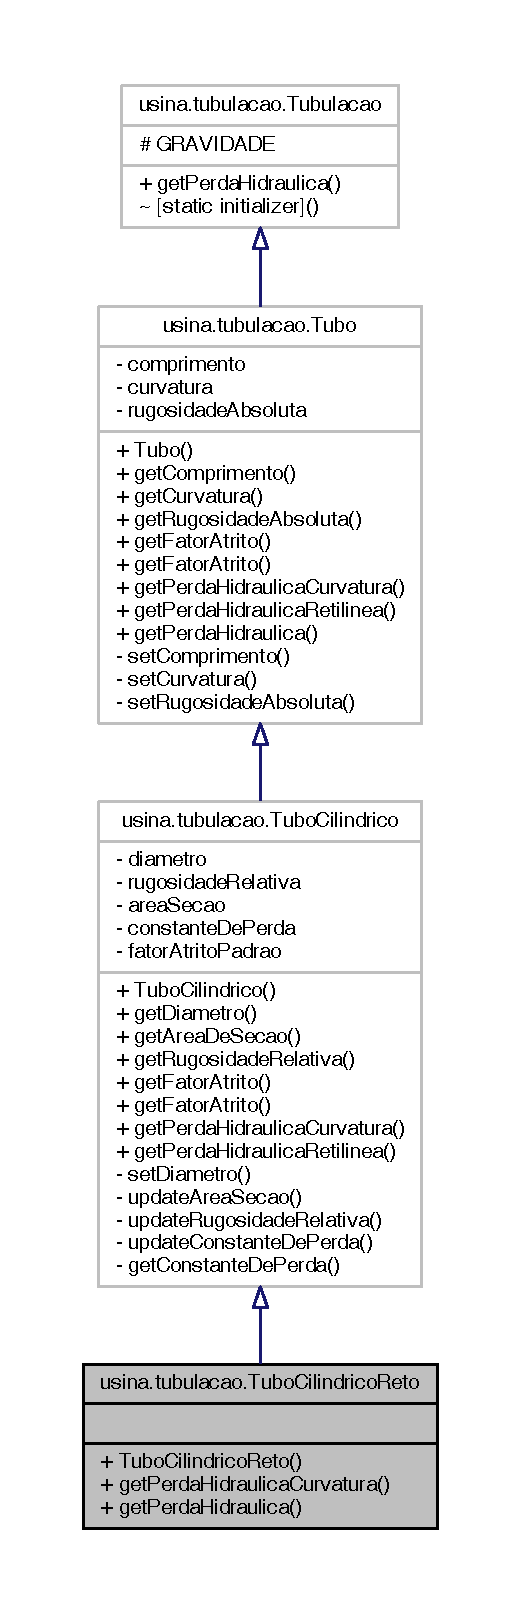
\includegraphics[height=550pt]{classusina_1_1tubulacao_1_1_tubo_cilindrico_reto__inherit__graph}
\end{center}
\end{figure}


Diagrama de colaboração para usina.\-tubulacao.\-Tubo\-Cilindrico\-Reto\-:\nopagebreak
\begin{figure}[H]
\begin{center}
\leavevmode
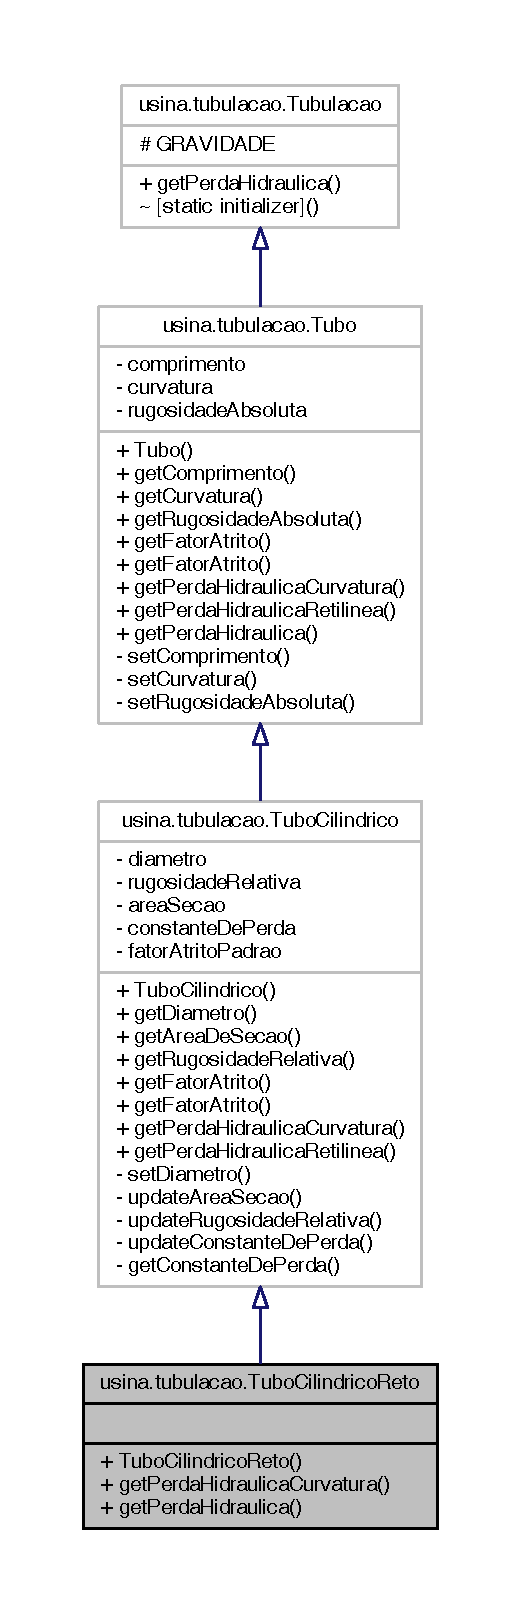
\includegraphics[height=550pt]{classusina_1_1tubulacao_1_1_tubo_cilindrico_reto__coll__graph}
\end{center}
\end{figure}
\subsection*{Métodos Públicos}
\begin{DoxyCompactItemize}
\item 
\hyperlink{classusina_1_1tubulacao_1_1_tubo_cilindrico_reto_a2d82044194c17e02787372c12fd55554}{Tubo\-Cilindrico\-Reto} (double comprimento, double diametro, double rugosidade\-Absoluta)
\begin{DoxyCompactList}\small\item\em Construtor. \end{DoxyCompactList}\item 
final double \hyperlink{classusina_1_1tubulacao_1_1_tubo_cilindrico_reto_ab7ba64d9ef5e97bbb8bb5a590b66eeb9}{get\-Perda\-Hidraulica\-Curvatura} (final \hyperlink{classusina_1_1_fluxo}{Fluxo} fluxo)
\item 
final double \hyperlink{classusina_1_1tubulacao_1_1_tubo_cilindrico_reto_a3dba7ffdcdaadb977f2f8b837905ae20}{get\-Perda\-Hidraulica} (final \hyperlink{classusina_1_1_fluxo}{Fluxo} fluxo)
\end{DoxyCompactItemize}


\subsection{Descrição Detalhada}
\begin{DoxyAuthor}{Autor}
Victor Soares 
\end{DoxyAuthor}
\begin{DoxyVersion}{Versão}
1.\-0 
\end{DoxyVersion}


\subsection{Construtores \& Destrutores}
\hypertarget{classusina_1_1tubulacao_1_1_tubo_cilindrico_reto_a2d82044194c17e02787372c12fd55554}{\index{usina\-::tubulacao\-::\-Tubo\-Cilindrico\-Reto@{usina\-::tubulacao\-::\-Tubo\-Cilindrico\-Reto}!Tubo\-Cilindrico\-Reto@{Tubo\-Cilindrico\-Reto}}
\index{Tubo\-Cilindrico\-Reto@{Tubo\-Cilindrico\-Reto}!usina::tubulacao::TuboCilindricoReto@{usina\-::tubulacao\-::\-Tubo\-Cilindrico\-Reto}}
\subsubsection[{Tubo\-Cilindrico\-Reto}]{\setlength{\rightskip}{0pt plus 5cm}usina.\-tubulacao.\-Tubo\-Cilindrico\-Reto.\-Tubo\-Cilindrico\-Reto (
\begin{DoxyParamCaption}
\item[{double}]{comprimento, }
\item[{double}]{diametro, }
\item[{double}]{rugosidade\-Absoluta}
\end{DoxyParamCaption}
)}}\label{classusina_1_1tubulacao_1_1_tubo_cilindrico_reto_a2d82044194c17e02787372c12fd55554}


Construtor. 


\begin{DoxyParams}{Parâmetros}
{\em comprimento} & Comprimento da tubula��o \mbox{[}m\mbox{]}. \\
\hline
{\em diametro} & Diametro \mbox{[}m\mbox{]}. \\
\hline
{\em rugosidade\-Absoluta} & Rugosidade Absoluta \mbox{[}m\mbox{]}. \\
\hline
\end{DoxyParams}
\begin{DoxySince}{Desde}
1.\-0 
\end{DoxySince}


\subsection{Métodos}
\hypertarget{classusina_1_1tubulacao_1_1_tubo_cilindrico_reto_a3dba7ffdcdaadb977f2f8b837905ae20}{\index{usina\-::tubulacao\-::\-Tubo\-Cilindrico\-Reto@{usina\-::tubulacao\-::\-Tubo\-Cilindrico\-Reto}!get\-Perda\-Hidraulica@{get\-Perda\-Hidraulica}}
\index{get\-Perda\-Hidraulica@{get\-Perda\-Hidraulica}!usina::tubulacao::TuboCilindricoReto@{usina\-::tubulacao\-::\-Tubo\-Cilindrico\-Reto}}
\subsubsection[{get\-Perda\-Hidraulica}]{\setlength{\rightskip}{0pt plus 5cm}final double usina.\-tubulacao.\-Tubo\-Cilindrico\-Reto.\-get\-Perda\-Hidraulica (
\begin{DoxyParamCaption}
\item[{final {\bf Fluxo}}]{fluxo}
\end{DoxyParamCaption}
)}}\label{classusina_1_1tubulacao_1_1_tubo_cilindrico_reto_a3dba7ffdcdaadb977f2f8b837905ae20}




\hypertarget{classusina_1_1tubulacao_1_1_tubo_cilindrico_reto_ab7ba64d9ef5e97bbb8bb5a590b66eeb9}{\index{usina\-::tubulacao\-::\-Tubo\-Cilindrico\-Reto@{usina\-::tubulacao\-::\-Tubo\-Cilindrico\-Reto}!get\-Perda\-Hidraulica\-Curvatura@{get\-Perda\-Hidraulica\-Curvatura}}
\index{get\-Perda\-Hidraulica\-Curvatura@{get\-Perda\-Hidraulica\-Curvatura}!usina::tubulacao::TuboCilindricoReto@{usina\-::tubulacao\-::\-Tubo\-Cilindrico\-Reto}}
\subsubsection[{get\-Perda\-Hidraulica\-Curvatura}]{\setlength{\rightskip}{0pt plus 5cm}final double usina.\-tubulacao.\-Tubo\-Cilindrico\-Reto.\-get\-Perda\-Hidraulica\-Curvatura (
\begin{DoxyParamCaption}
\item[{final {\bf Fluxo}}]{fluxo}
\end{DoxyParamCaption}
)}}\label{classusina_1_1tubulacao_1_1_tubo_cilindrico_reto_ab7ba64d9ef5e97bbb8bb5a590b66eeb9}






A documentação para esta classe foi gerada a partir do seguinte arquivo\-:\begin{DoxyCompactItemize}
\item 
C\-:/\-Users/\-Victor/workplace/\-Net\-Beans\-Projects/tcc/src/usina/tubulacao/\hyperlink{_tubo_cilindrico_reto_8java}{Tubo\-Cilindrico\-Reto.\-java}\end{DoxyCompactItemize}

\hypertarget{classusina_1_1_turbina}{\section{Referência da Classe usina.\-Turbina}
\label{classusina_1_1_turbina}\index{usina.\-Turbina@{usina.\-Turbina}}
}


Conjunto turbina-\/gerador.  




Diagrama de colaboração para usina.\-Turbina\-:
\nopagebreak
\begin{figure}[H]
\begin{center}
\leavevmode
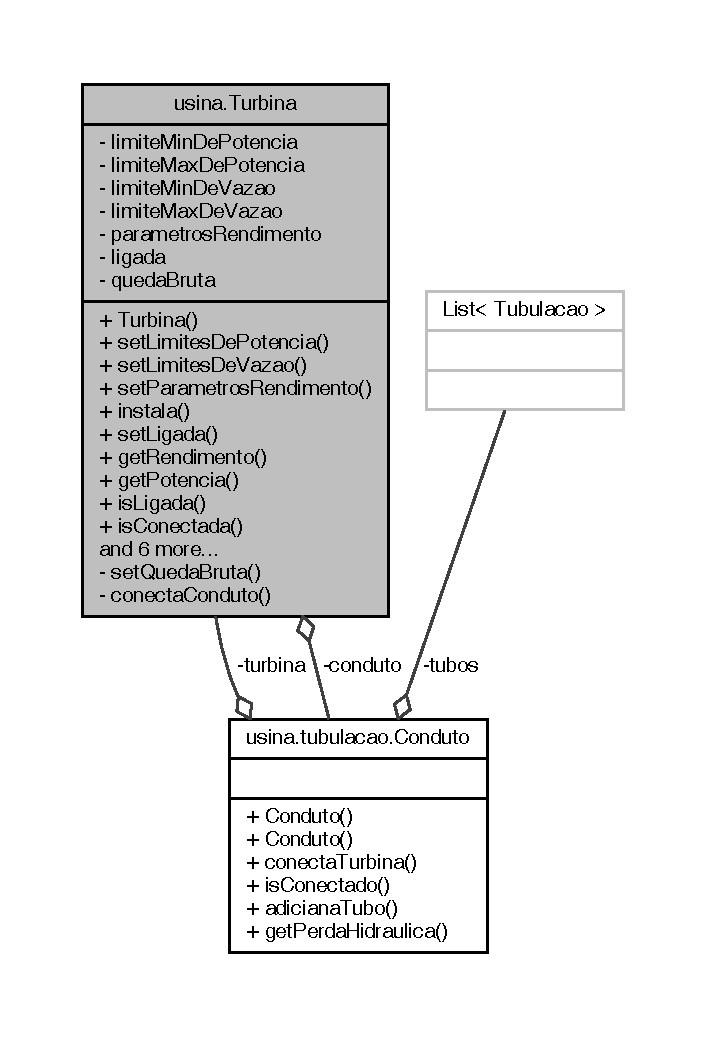
\includegraphics[width=339pt]{classusina_1_1_turbina__coll__graph}
\end{center}
\end{figure}
\subsection*{Métodos Públicos}
\begin{DoxyCompactItemize}
\item 
\hyperlink{classusina_1_1_turbina_abd3ec63d990bd3598954031d6daffabc}{Turbina} (Double \hyperlink{classusina_1_1_turbina_a9d422881e2943b12a26cb27caf92d08b}{limite\-Min\-De\-Potencia}, Double \hyperlink{classusina_1_1_turbina_ab6648bca34b30eedf9f9246fe7bfde00}{limite\-Max\-De\-Potencia}, Double \hyperlink{classusina_1_1_turbina_a549b44e83d93c34fc79bdeb688c60b7d}{limite\-Min\-De\-Vazao}, Double \hyperlink{classusina_1_1_turbina_a0f961379b5f4e4779f98d15dd093c6ba}{limite\-Max\-De\-Vazao}, Double\mbox{[}$\,$\mbox{]} \hyperlink{classusina_1_1_turbina_a5787dbae79e4108296573fd4dbf156da}{parametros\-Rendimento})
\begin{DoxyCompactList}\small\item\em Construtor. \end{DoxyCompactList}\item 
final void \hyperlink{classusina_1_1_turbina_af3c11239f2309b85267bdc60580bd9a8}{set\-Limites\-De\-Potencia} (Double \hyperlink{classusina_1_1_turbina_a9d422881e2943b12a26cb27caf92d08b}{limite\-Min\-De\-Potencia}, Double \hyperlink{classusina_1_1_turbina_ab6648bca34b30eedf9f9246fe7bfde00}{limite\-Max\-De\-Potencia})
\begin{DoxyCompactList}\small\item\em Atribui limites à potência da turbina. \end{DoxyCompactList}\item 
final void \hyperlink{classusina_1_1_turbina_a7b96c0bc6e3eff9430d79d287645c306}{set\-Limites\-De\-Vazao} (Double \hyperlink{classusina_1_1_turbina_a549b44e83d93c34fc79bdeb688c60b7d}{limite\-Min\-De\-Vazao}, Double \hyperlink{classusina_1_1_turbina_a0f961379b5f4e4779f98d15dd093c6ba}{limite\-Max\-De\-Vazao})
\begin{DoxyCompactList}\small\item\em Atribui limites à vazão da turbina. \end{DoxyCompactList}\item 
void \hyperlink{classusina_1_1_turbina_abc98fbb1a34b3d911b791e6a19f9c784}{set\-Parametros\-Rendimento} (Double\mbox{[}$\,$\mbox{]} \hyperlink{classusina_1_1_turbina_a5787dbae79e4108296573fd4dbf156da}{parametros\-Rendimento})
\begin{DoxyCompactList}\small\item\em Atribui os parâmetros para o calculo do get\-Rendimento. \end{DoxyCompactList}\item 
final void \hyperlink{classusina_1_1_turbina_ad46569765ed883b27b39096e6e30ffe9}{instala} (Double \hyperlink{classusina_1_1_turbina_a74ca99529c8c56c1ffddba8bc914c442}{queda\-Bruta}, \hyperlink{classusina_1_1tubulacao_1_1_conduto}{Conduto} \hyperlink{classusina_1_1_turbina_aaf9ebcc66e369abbf1ccf644579e1348}{conduto})
\begin{DoxyCompactList}\small\item\em Instala turbina na usina por meio de um conduto. \end{DoxyCompactList}\item 
final void \hyperlink{classusina_1_1_turbina_aef2a44bda149b3bd9afd627145b53df2}{set\-Ligada} (Boolean \hyperlink{classusina_1_1_turbina_afe4aa27ba1150a9b4a2a7d9ec622ab4f}{ligada})
\begin{DoxyCompactList}\small\item\em Controla o estado de uma turbina, ligando ou desligando a mesma. \end{DoxyCompactList}\item 
final Double \hyperlink{classusina_1_1_turbina_ad7eb2929acee76d69ef06d67c01d0e1a}{get\-Rendimento} (\hyperlink{classusina_1_1_fluxo}{Fluxo} fluxo)
\begin{DoxyCompactList}\small\item\em Calcula o rendimento da turbina dado um fluxo. \end{DoxyCompactList}\item 
final Double \hyperlink{classusina_1_1_turbina_ab5f2692c54cf1e3fe6b30adc3b481710}{get\-Potencia} (\hyperlink{classusina_1_1_fluxo}{Fluxo} fluxo)
\begin{DoxyCompactList}\small\item\em Calcula a potência gerada da turbina dado um fluxo. \end{DoxyCompactList}\item 
final Boolean \hyperlink{classusina_1_1_turbina_a62d5a81d710e36542ca8a001bf16a3e1}{is\-Ligada} ()
\begin{DoxyCompactList}\small\item\em Verifica o estado da turbina, ligada/desligada. \end{DoxyCompactList}\item 
Boolean \hyperlink{classusina_1_1_turbina_aab5ba2c5ccb1f98ea31928d3197f8a88}{is\-Conectada} ()
\begin{DoxyCompactList}\small\item\em Verifica o estado da turbina, conectada ou desconectada. \end{DoxyCompactList}\item 
final Double \hyperlink{classusina_1_1_turbina_aee3faa93f4d92db651edbea96d1df938}{get\-Limite\-Min\-De\-Potencia} ()
\begin{DoxyCompactList}\small\item\em Recupera o limite mínimo de potência para operação da turbina. \end{DoxyCompactList}\item 
final Double \hyperlink{classusina_1_1_turbina_ae08079645408277e5f4b34869c8fbdbc}{get\-Limite\-Max\-De\-Potencia} ()
\begin{DoxyCompactList}\small\item\em Recupera o limite máximo de potência para operação da turbina. \end{DoxyCompactList}\item 
final Double \hyperlink{classusina_1_1_turbina_a62be0e3ac4c6461fc2202b6b97cbf8ec}{get\-Limite\-Min\-De\-Vazao} ()
\begin{DoxyCompactList}\small\item\em Recupera o limite mínimo de vazão para operação da turbina. \end{DoxyCompactList}\item 
final Double \hyperlink{classusina_1_1_turbina_aa13d59b00e57632fcfc9db6f651d4a9d}{get\-Limite\-Max\-De\-Vazao} ()
\begin{DoxyCompactList}\small\item\em Recupera o limite máximo de vazão para operação da turbina. \end{DoxyCompactList}\item 
final Double \hyperlink{classusina_1_1_turbina_aa31333043136ac0d431d3347099e268e}{get\-Queda\-Bruta} ()
\begin{DoxyCompactList}\small\item\em Recupera a queda bruta, definida na instalação. \end{DoxyCompactList}\item 
String \hyperlink{classusina_1_1_turbina_af0070ee6333afe97856a58e309e72064}{to\-String} ()
\end{DoxyCompactItemize}
\subsection*{Métodos Privados}
\begin{DoxyCompactItemize}
\item 
void \hyperlink{classusina_1_1_turbina_a373df75de3c1226b0d518254ae3831bf}{set\-Queda\-Bruta} (Double \hyperlink{classusina_1_1_turbina_a74ca99529c8c56c1ffddba8bc914c442}{queda\-Bruta})
\begin{DoxyCompactList}\small\item\em Define a queda bruta no momento da instalação. \end{DoxyCompactList}\item 
void \hyperlink{classusina_1_1_turbina_a15f7eae41d56f2cbb7a271a3af549350}{conecta\-Conduto} (\hyperlink{classusina_1_1tubulacao_1_1_conduto}{Conduto} \hyperlink{classusina_1_1_turbina_aaf9ebcc66e369abbf1ccf644579e1348}{conduto})
\begin{DoxyCompactList}\small\item\em Conecta a turbina a um conduto no momento da instalação. \end{DoxyCompactList}\end{DoxyCompactItemize}
\subsection*{Atributos Privados}
\begin{DoxyCompactItemize}
\item 
Double \hyperlink{classusina_1_1_turbina_a9d422881e2943b12a26cb27caf92d08b}{limite\-Min\-De\-Potencia}
\item 
Double \hyperlink{classusina_1_1_turbina_ab6648bca34b30eedf9f9246fe7bfde00}{limite\-Max\-De\-Potencia}
\item 
Double \hyperlink{classusina_1_1_turbina_a549b44e83d93c34fc79bdeb688c60b7d}{limite\-Min\-De\-Vazao}
\item 
Double \hyperlink{classusina_1_1_turbina_a0f961379b5f4e4779f98d15dd093c6ba}{limite\-Max\-De\-Vazao}
\item 
Double\mbox{[}$\,$\mbox{]} \hyperlink{classusina_1_1_turbina_a5787dbae79e4108296573fd4dbf156da}{parametros\-Rendimento}
\item 
Boolean \hyperlink{classusina_1_1_turbina_afe4aa27ba1150a9b4a2a7d9ec622ab4f}{ligada}
\item 
Double \hyperlink{classusina_1_1_turbina_a74ca99529c8c56c1ffddba8bc914c442}{queda\-Bruta}
\item 
\hyperlink{classusina_1_1tubulacao_1_1_conduto}{Conduto} \hyperlink{classusina_1_1_turbina_aaf9ebcc66e369abbf1ccf644579e1348}{conduto}
\end{DoxyCompactItemize}


\subsection{Descrição Detalhada}
Conjunto turbina-\/gerador. 

Classe representante dos conjuntos geradores no problema de despacho elétrico. 

Usa-\/se, aqui, por simplicidade, os substantivos turbina e conjunto-\/gerador como sinônimos. Uma divisão mais detalhada seria desnecessária, pois o modelo atual trata da eficiência do conjunto. 

\begin{DoxyAuthor}{Autor}
Victor de Lima Soares 
\end{DoxyAuthor}
\begin{DoxyVersion}{Versão}
1.\-0 
\end{DoxyVersion}


\subsection{Construtores \& Destrutores}
\hypertarget{classusina_1_1_turbina_abd3ec63d990bd3598954031d6daffabc}{\index{usina\-::\-Turbina@{usina\-::\-Turbina}!Turbina@{Turbina}}
\index{Turbina@{Turbina}!usina::Turbina@{usina\-::\-Turbina}}
\subsubsection[{Turbina}]{\setlength{\rightskip}{0pt plus 5cm}usina.\-Turbina.\-Turbina (
\begin{DoxyParamCaption}
\item[{Double}]{limite\-Min\-De\-Potencia, }
\item[{Double}]{limite\-Max\-De\-Potencia, }
\item[{Double}]{limite\-Min\-De\-Vazao, }
\item[{Double}]{limite\-Max\-De\-Vazao, }
\item[{Double\mbox{[}$\,$\mbox{]}}]{parametros\-Rendimento}
\end{DoxyParamCaption}
)}}\label{classusina_1_1_turbina_abd3ec63d990bd3598954031d6daffabc}


Construtor. 

Por padrão uma turbina é instanciada como desligada e desconectada. 


\begin{DoxyParams}{Parâmetros}
{\em limite\-Min\-De\-Potencia} & Limite inferior para potência, inclusive. \\
\hline
{\em limite\-Max\-De\-Potencia} & Limite superior para potência, exclusive. \\
\hline
{\em limite\-Min\-De\-Vazao} & Limite inferior para vazão, inclusive. \\
\hline
{\em limite\-Max\-De\-Vazao} & Limite superior para vazão, exclusive. \\
\hline
{\em parametros\-Rendimento} & Parâmetros para calculo do get\-Rendimento.\\
\hline
\end{DoxyParams}
\begin{DoxySeeAlso}{Veja também}
\hyperlink{classusina_1_1_turbina_ad7eb2929acee76d69ef06d67c01d0e1a}{get\-Rendimento}(\hyperlink{classusina_1_1_fluxo}{usina.\-Fluxo}) 

\hyperlink{classusina_1_1_turbina_ad46569765ed883b27b39096e6e30ffe9}{instala}(java.\-lang.\-Double, \hyperlink{classusina_1_1tubulacao_1_1_conduto}{usina.\-tubulacao.\-Conduto}) 

\hyperlink{classusina_1_1_turbina_aef2a44bda149b3bd9afd627145b53df2}{set\-Ligada}(java.\-lang.\-Boolean) 
\end{DoxySeeAlso}


Este é o diagrama das funções utilizadas por esta função\-:
\nopagebreak
\begin{figure}[H]
\begin{center}
\leavevmode
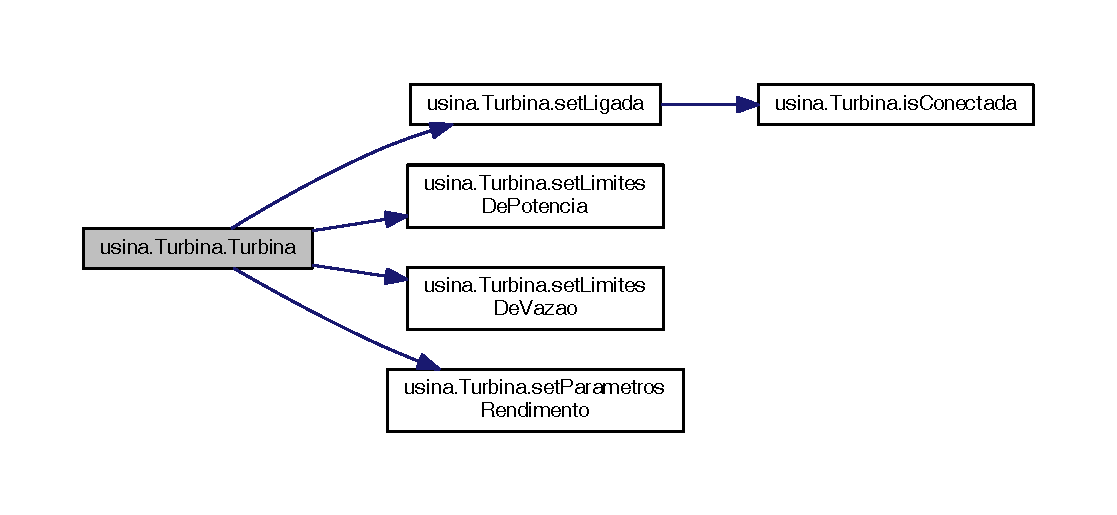
\includegraphics[width=350pt]{classusina_1_1_turbina_abd3ec63d990bd3598954031d6daffabc_cgraph}
\end{center}
\end{figure}




\subsection{Métodos}
\hypertarget{classusina_1_1_turbina_a15f7eae41d56f2cbb7a271a3af549350}{\index{usina\-::\-Turbina@{usina\-::\-Turbina}!conecta\-Conduto@{conecta\-Conduto}}
\index{conecta\-Conduto@{conecta\-Conduto}!usina::Turbina@{usina\-::\-Turbina}}
\subsubsection[{conecta\-Conduto}]{\setlength{\rightskip}{0pt plus 5cm}void usina.\-Turbina.\-conecta\-Conduto (
\begin{DoxyParamCaption}
\item[{{\bf Conduto}}]{conduto}
\end{DoxyParamCaption}
)\hspace{0.3cm}{\ttfamily [private]}}}\label{classusina_1_1_turbina_a15f7eae41d56f2cbb7a271a3af549350}


Conecta a turbina a um conduto no momento da instalação. 

{\bfseries Não pode ser usada mais de uma vez.} 

\begin{DoxySince}{Desde}
1.\-0 
\end{DoxySince}

\begin{DoxyParams}{Parâmetros}
{\em conduto} & Conduto onde a turbina será instalada. \\
\hline
\end{DoxyParams}

\begin{DoxyExceptions}{Exceções}
{\em Illegal\-State\-Exception} & 
\begin{DoxyItemize}
\item Se a turbina já estiver conectada a outro conduto. 
\end{DoxyItemize}\\
\hline
{\em Null\-Pointer\-Exception} & 
\begin{DoxyItemize}
\item Se a referência para o conduto for nula. 
\end{DoxyItemize}\\
\hline
\end{DoxyExceptions}


Este é o diagrama das funções utilizadas por esta função\-:\nopagebreak
\begin{figure}[H]
\begin{center}
\leavevmode
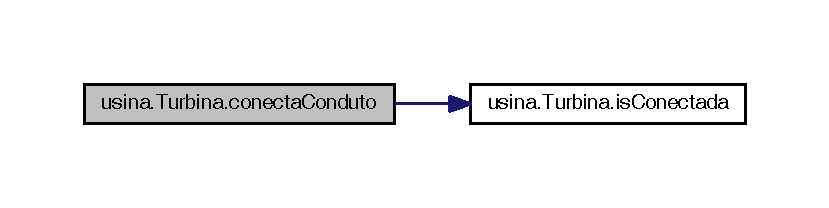
\includegraphics[width=350pt]{classusina_1_1_turbina_a15f7eae41d56f2cbb7a271a3af549350_cgraph}
\end{center}
\end{figure}




Este é o diagrama das funções que utilizam esta função\-:\nopagebreak
\begin{figure}[H]
\begin{center}
\leavevmode
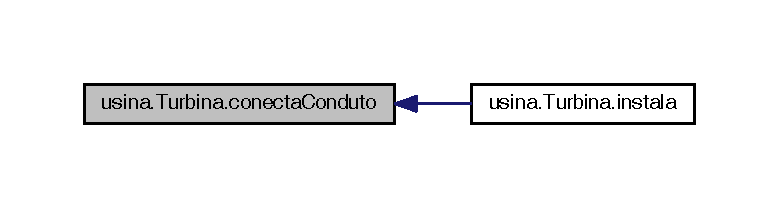
\includegraphics[width=350pt]{classusina_1_1_turbina_a15f7eae41d56f2cbb7a271a3af549350_icgraph}
\end{center}
\end{figure}


\hypertarget{classusina_1_1_turbina_ae08079645408277e5f4b34869c8fbdbc}{\index{usina\-::\-Turbina@{usina\-::\-Turbina}!get\-Limite\-Max\-De\-Potencia@{get\-Limite\-Max\-De\-Potencia}}
\index{get\-Limite\-Max\-De\-Potencia@{get\-Limite\-Max\-De\-Potencia}!usina::Turbina@{usina\-::\-Turbina}}
\subsubsection[{get\-Limite\-Max\-De\-Potencia}]{\setlength{\rightskip}{0pt plus 5cm}final Double usina.\-Turbina.\-get\-Limite\-Max\-De\-Potencia (
\begin{DoxyParamCaption}
{}
\end{DoxyParamCaption}
)}}\label{classusina_1_1_turbina_ae08079645408277e5f4b34869c8fbdbc}


Recupera o limite máximo de potência para operação da turbina. 

\begin{DoxySince}{Desde}
1.\-0 
\end{DoxySince}
\begin{DoxyReturn}{Retorna}
Limite máximo de potência. 
\end{DoxyReturn}
\hypertarget{classusina_1_1_turbina_aa13d59b00e57632fcfc9db6f651d4a9d}{\index{usina\-::\-Turbina@{usina\-::\-Turbina}!get\-Limite\-Max\-De\-Vazao@{get\-Limite\-Max\-De\-Vazao}}
\index{get\-Limite\-Max\-De\-Vazao@{get\-Limite\-Max\-De\-Vazao}!usina::Turbina@{usina\-::\-Turbina}}
\subsubsection[{get\-Limite\-Max\-De\-Vazao}]{\setlength{\rightskip}{0pt plus 5cm}final Double usina.\-Turbina.\-get\-Limite\-Max\-De\-Vazao (
\begin{DoxyParamCaption}
{}
\end{DoxyParamCaption}
)}}\label{classusina_1_1_turbina_aa13d59b00e57632fcfc9db6f651d4a9d}


Recupera o limite máximo de vazão para operação da turbina. 

\begin{DoxySince}{Desde}
1.\-0 
\end{DoxySince}
\begin{DoxyReturn}{Retorna}
Limite máximo de vazão. 
\end{DoxyReturn}
\hypertarget{classusina_1_1_turbina_aee3faa93f4d92db651edbea96d1df938}{\index{usina\-::\-Turbina@{usina\-::\-Turbina}!get\-Limite\-Min\-De\-Potencia@{get\-Limite\-Min\-De\-Potencia}}
\index{get\-Limite\-Min\-De\-Potencia@{get\-Limite\-Min\-De\-Potencia}!usina::Turbina@{usina\-::\-Turbina}}
\subsubsection[{get\-Limite\-Min\-De\-Potencia}]{\setlength{\rightskip}{0pt plus 5cm}final Double usina.\-Turbina.\-get\-Limite\-Min\-De\-Potencia (
\begin{DoxyParamCaption}
{}
\end{DoxyParamCaption}
)}}\label{classusina_1_1_turbina_aee3faa93f4d92db651edbea96d1df938}


Recupera o limite mínimo de potência para operação da turbina. 

\begin{DoxySince}{Desde}
1.\-0 
\end{DoxySince}
\begin{DoxyReturn}{Retorna}
Limite mínimo de potência. 
\end{DoxyReturn}
\hypertarget{classusina_1_1_turbina_a62be0e3ac4c6461fc2202b6b97cbf8ec}{\index{usina\-::\-Turbina@{usina\-::\-Turbina}!get\-Limite\-Min\-De\-Vazao@{get\-Limite\-Min\-De\-Vazao}}
\index{get\-Limite\-Min\-De\-Vazao@{get\-Limite\-Min\-De\-Vazao}!usina::Turbina@{usina\-::\-Turbina}}
\subsubsection[{get\-Limite\-Min\-De\-Vazao}]{\setlength{\rightskip}{0pt plus 5cm}final Double usina.\-Turbina.\-get\-Limite\-Min\-De\-Vazao (
\begin{DoxyParamCaption}
{}
\end{DoxyParamCaption}
)}}\label{classusina_1_1_turbina_a62be0e3ac4c6461fc2202b6b97cbf8ec}


Recupera o limite mínimo de vazão para operação da turbina. 

\begin{DoxySince}{Desde}
1.\-0 
\end{DoxySince}
\begin{DoxyReturn}{Retorna}
Limite mínimo de vazão. 
\end{DoxyReturn}


Este é o diagrama das funções que utilizam esta função\-:\nopagebreak
\begin{figure}[H]
\begin{center}
\leavevmode
\includegraphics[width=350pt]{classusina_1_1_turbina_a62be0e3ac4c6461fc2202b6b97cbf8ec_icgraph}
\end{center}
\end{figure}


\hypertarget{classusina_1_1_turbina_ab5f2692c54cf1e3fe6b30adc3b481710}{\index{usina\-::\-Turbina@{usina\-::\-Turbina}!get\-Potencia@{get\-Potencia}}
\index{get\-Potencia@{get\-Potencia}!usina::Turbina@{usina\-::\-Turbina}}
\subsubsection[{get\-Potencia}]{\setlength{\rightskip}{0pt plus 5cm}final Double usina.\-Turbina.\-get\-Potencia (
\begin{DoxyParamCaption}
\item[{{\bf Fluxo}}]{fluxo}
\end{DoxyParamCaption}
)}}\label{classusina_1_1_turbina_ab5f2692c54cf1e3fe6b30adc3b481710}


Calcula a potência gerada da turbina dado um fluxo. 

\begin{DoxySince}{Desde}
1.\-0 
\end{DoxySince}

\begin{DoxyParams}{Parâmetros}
{\em fluxo} & \hyperlink{classusina_1_1_fluxo}{Fluxo} de parametrização. \\
\hline
\end{DoxyParams}
\begin{DoxyReturn}{Retorna}
Potência da turbina. 
\end{DoxyReturn}


Este é o diagrama das funções utilizadas por esta função\-:
\nopagebreak
\begin{figure}[H]
\begin{center}
\leavevmode
\includegraphics[width=350pt]{classusina_1_1_turbina_ab5f2692c54cf1e3fe6b30adc3b481710_cgraph}
\end{center}
\end{figure}


\hypertarget{classusina_1_1_turbina_aa31333043136ac0d431d3347099e268e}{\index{usina\-::\-Turbina@{usina\-::\-Turbina}!get\-Queda\-Bruta@{get\-Queda\-Bruta}}
\index{get\-Queda\-Bruta@{get\-Queda\-Bruta}!usina::Turbina@{usina\-::\-Turbina}}
\subsubsection[{get\-Queda\-Bruta}]{\setlength{\rightskip}{0pt plus 5cm}final Double usina.\-Turbina.\-get\-Queda\-Bruta (
\begin{DoxyParamCaption}
{}
\end{DoxyParamCaption}
)}}\label{classusina_1_1_turbina_aa31333043136ac0d431d3347099e268e}


Recupera a queda bruta, definida na instalação. 

\begin{DoxySince}{Desde}
1.\-0 
\end{DoxySince}
\begin{DoxyReturn}{Retorna}
A queda bruta. 
\end{DoxyReturn}


Este é o diagrama das funções que utilizam esta função\-:
\nopagebreak
\begin{figure}[H]
\begin{center}
\leavevmode
\includegraphics[width=350pt]{classusina_1_1_turbina_aa31333043136ac0d431d3347099e268e_icgraph}
\end{center}
\end{figure}


\hypertarget{classusina_1_1_turbina_ad7eb2929acee76d69ef06d67c01d0e1a}{\index{usina\-::\-Turbina@{usina\-::\-Turbina}!get\-Rendimento@{get\-Rendimento}}
\index{get\-Rendimento@{get\-Rendimento}!usina::Turbina@{usina\-::\-Turbina}}
\subsubsection[{get\-Rendimento}]{\setlength{\rightskip}{0pt plus 5cm}final Double usina.\-Turbina.\-get\-Rendimento (
\begin{DoxyParamCaption}
\item[{{\bf Fluxo}}]{fluxo}
\end{DoxyParamCaption}
)}}\label{classusina_1_1_turbina_ad7eb2929acee76d69ef06d67c01d0e1a}


Calcula o rendimento da turbina dado um fluxo. 

\begin{DoxySince}{Desde}
1.\-0 
\end{DoxySince}

\begin{DoxyParams}{Parâmetros}
{\em fluxo} & \hyperlink{classusina_1_1_fluxo}{Fluxo} de parametrização. \\
\hline
\end{DoxyParams}
\begin{DoxyReturn}{Retorna}
Rendimento da turbina. 
\end{DoxyReturn}


Este é o diagrama das funções utilizadas por esta função\-:
\nopagebreak
\begin{figure}[H]
\begin{center}
\leavevmode
\includegraphics[width=350pt]{classusina_1_1_turbina_ad7eb2929acee76d69ef06d67c01d0e1a_cgraph}
\end{center}
\end{figure}




Este é o diagrama das funções que utilizam esta função\-:
\nopagebreak
\begin{figure}[H]
\begin{center}
\leavevmode
\includegraphics[width=350pt]{classusina_1_1_turbina_ad7eb2929acee76d69ef06d67c01d0e1a_icgraph}
\end{center}
\end{figure}


\hypertarget{classusina_1_1_turbina_ad46569765ed883b27b39096e6e30ffe9}{\index{usina\-::\-Turbina@{usina\-::\-Turbina}!instala@{instala}}
\index{instala@{instala}!usina::Turbina@{usina\-::\-Turbina}}
\subsubsection[{instala}]{\setlength{\rightskip}{0pt plus 5cm}final void usina.\-Turbina.\-instala (
\begin{DoxyParamCaption}
\item[{Double}]{queda\-Bruta, }
\item[{{\bf Conduto}}]{conduto}
\end{DoxyParamCaption}
)}}\label{classusina_1_1_turbina_ad46569765ed883b27b39096e6e30ffe9}


Instala turbina na usina por meio de um conduto. 

{\bfseries Não pode ser usada mais de uma vez.} 

\begin{DoxySince}{Desde}
1.\-0 
\end{DoxySince}

\begin{DoxyParams}{Parâmetros}
{\em queda\-Bruta} & A queda bruta na operação da turbina. \\
\hline
{\em conduto} & Conduto onde a turbina será instalada.\\
\hline
\end{DoxyParams}

\begin{DoxyExceptions}{Exceções}
{\em Illegal\-Argument\-Exception} & 
\begin{DoxyItemize}
\item Se a queda bruta for menor que zero. 
\end{DoxyItemize}\\
\hline
{\em Illegal\-State\-Exception} & 
\begin{DoxyItemize}
\item Se a função for usada mais de uma vez; 
\item Se a turbina já estiver conectada a outro conduto. 
\end{DoxyItemize}\\
\hline
{\em Null\-Pointer\-Exception} & 
\begin{DoxyItemize}
\item Se a referência para o conduto for nula. 
\end{DoxyItemize}\\
\hline
\end{DoxyExceptions}


Este é o diagrama das funções utilizadas por esta função\-:\nopagebreak
\begin{figure}[H]
\begin{center}
\leavevmode
\includegraphics[width=350pt]{classusina_1_1_turbina_ad46569765ed883b27b39096e6e30ffe9_cgraph}
\end{center}
\end{figure}


\hypertarget{classusina_1_1_turbina_aab5ba2c5ccb1f98ea31928d3197f8a88}{\index{usina\-::\-Turbina@{usina\-::\-Turbina}!is\-Conectada@{is\-Conectada}}
\index{is\-Conectada@{is\-Conectada}!usina::Turbina@{usina\-::\-Turbina}}
\subsubsection[{is\-Conectada}]{\setlength{\rightskip}{0pt plus 5cm}Boolean usina.\-Turbina.\-is\-Conectada (
\begin{DoxyParamCaption}
{}
\end{DoxyParamCaption}
)}}\label{classusina_1_1_turbina_aab5ba2c5ccb1f98ea31928d3197f8a88}


Verifica o estado da turbina, conectada ou desconectada. 

\begin{DoxyReturn}{Retorna}
Estado da turbina\-: 
\begin{DoxyItemize}
\item True\-: conectada. 
\item False\-: desconectada. 
\end{DoxyItemize}
\end{DoxyReturn}


Este é o diagrama das funções que utilizam esta função\-:\nopagebreak
\begin{figure}[H]
\begin{center}
\leavevmode
\includegraphics[width=350pt]{classusina_1_1_turbina_aab5ba2c5ccb1f98ea31928d3197f8a88_icgraph}
\end{center}
\end{figure}


\hypertarget{classusina_1_1_turbina_a62d5a81d710e36542ca8a001bf16a3e1}{\index{usina\-::\-Turbina@{usina\-::\-Turbina}!is\-Ligada@{is\-Ligada}}
\index{is\-Ligada@{is\-Ligada}!usina::Turbina@{usina\-::\-Turbina}}
\subsubsection[{is\-Ligada}]{\setlength{\rightskip}{0pt plus 5cm}final Boolean usina.\-Turbina.\-is\-Ligada (
\begin{DoxyParamCaption}
{}
\end{DoxyParamCaption}
)}}\label{classusina_1_1_turbina_a62d5a81d710e36542ca8a001bf16a3e1}


Verifica o estado da turbina, ligada/desligada. 

\begin{DoxySince}{Desde}
1.\-0 
\end{DoxySince}
\begin{DoxyReturn}{Retorna}
Estado da turbina\-: 
\begin{DoxyItemize}
\item True\-: Ligada. 
\item False\-: Desligada. 
\end{DoxyItemize}
\end{DoxyReturn}


Este é o diagrama das funções que utilizam esta função\-:\nopagebreak
\begin{figure}[H]
\begin{center}
\leavevmode
\includegraphics[width=342pt]{classusina_1_1_turbina_a62d5a81d710e36542ca8a001bf16a3e1_icgraph}
\end{center}
\end{figure}


\hypertarget{classusina_1_1_turbina_aef2a44bda149b3bd9afd627145b53df2}{\index{usina\-::\-Turbina@{usina\-::\-Turbina}!set\-Ligada@{set\-Ligada}}
\index{set\-Ligada@{set\-Ligada}!usina::Turbina@{usina\-::\-Turbina}}
\subsubsection[{set\-Ligada}]{\setlength{\rightskip}{0pt plus 5cm}final void usina.\-Turbina.\-set\-Ligada (
\begin{DoxyParamCaption}
\item[{Boolean}]{ligada}
\end{DoxyParamCaption}
)}}\label{classusina_1_1_turbina_aef2a44bda149b3bd9afd627145b53df2}


Controla o estado de uma turbina, ligando ou desligando a mesma. 

\begin{DoxySince}{Desde}
1.\-0 
\end{DoxySince}

\begin{DoxyParams}{Parâmetros}
{\em ligada} & Estado da turbina\-: ligado/desligado; 
\begin{DoxyItemize}
\item True\-: Liga turbina. 
\item False\-: Desliga turbina. 
\end{DoxyItemize}\\
\hline
\end{DoxyParams}

\begin{DoxyExceptions}{Exceções}
{\em Illegal\-State\-Exception} & 
\begin{DoxyItemize}
\item Se a turbina não estiver instalada. 
\end{DoxyItemize}\\
\hline
\end{DoxyExceptions}


Este é o diagrama das funções utilizadas por esta função\-:\nopagebreak
\begin{figure}[H]
\begin{center}
\leavevmode
\includegraphics[width=350pt]{classusina_1_1_turbina_aef2a44bda149b3bd9afd627145b53df2_cgraph}
\end{center}
\end{figure}




Este é o diagrama das funções que utilizam esta função\-:\nopagebreak
\begin{figure}[H]
\begin{center}
\leavevmode
\includegraphics[width=346pt]{classusina_1_1_turbina_aef2a44bda149b3bd9afd627145b53df2_icgraph}
\end{center}
\end{figure}


\hypertarget{classusina_1_1_turbina_af3c11239f2309b85267bdc60580bd9a8}{\index{usina\-::\-Turbina@{usina\-::\-Turbina}!set\-Limites\-De\-Potencia@{set\-Limites\-De\-Potencia}}
\index{set\-Limites\-De\-Potencia@{set\-Limites\-De\-Potencia}!usina::Turbina@{usina\-::\-Turbina}}
\subsubsection[{set\-Limites\-De\-Potencia}]{\setlength{\rightskip}{0pt plus 5cm}final void usina.\-Turbina.\-set\-Limites\-De\-Potencia (
\begin{DoxyParamCaption}
\item[{Double}]{limite\-Min\-De\-Potencia, }
\item[{Double}]{limite\-Max\-De\-Potencia}
\end{DoxyParamCaption}
)}}\label{classusina_1_1_turbina_af3c11239f2309b85267bdc60580bd9a8}


Atribui limites à potência da turbina. 

\begin{DoxySince}{Desde}
1.\-0 
\end{DoxySince}

\begin{DoxyParams}{Parâmetros}
{\em limite\-Min\-De\-Potencia} & Limite mínimo de potência para operação da turbina. \\
\hline
{\em limite\-Max\-De\-Potencia} & Limite máximo de potência para operação da turbina. \\
\hline
\end{DoxyParams}

\begin{DoxyExceptions}{Exceções}
{\em Illegal\-Argument\-Exception} & 
\begin{DoxyItemize}
\item Se o limite mínimo for menor que zero; 
\item Se o limite máximo for menor ou igual a zero; 
\item Se o limite máximo for menor que o limite mínimo. 
\end{DoxyItemize}\\
\hline
\end{DoxyExceptions}


Este é o diagrama das funções que utilizam esta função\-:\nopagebreak
\begin{figure}[H]
\begin{center}
\leavevmode
\includegraphics[width=350pt]{classusina_1_1_turbina_af3c11239f2309b85267bdc60580bd9a8_icgraph}
\end{center}
\end{figure}


\hypertarget{classusina_1_1_turbina_a7b96c0bc6e3eff9430d79d287645c306}{\index{usina\-::\-Turbina@{usina\-::\-Turbina}!set\-Limites\-De\-Vazao@{set\-Limites\-De\-Vazao}}
\index{set\-Limites\-De\-Vazao@{set\-Limites\-De\-Vazao}!usina::Turbina@{usina\-::\-Turbina}}
\subsubsection[{set\-Limites\-De\-Vazao}]{\setlength{\rightskip}{0pt plus 5cm}final void usina.\-Turbina.\-set\-Limites\-De\-Vazao (
\begin{DoxyParamCaption}
\item[{Double}]{limite\-Min\-De\-Vazao, }
\item[{Double}]{limite\-Max\-De\-Vazao}
\end{DoxyParamCaption}
)}}\label{classusina_1_1_turbina_a7b96c0bc6e3eff9430d79d287645c306}


Atribui limites à vazão da turbina. 

\begin{DoxySince}{Desde}
1.\-0 
\end{DoxySince}

\begin{DoxyParams}{Parâmetros}
{\em limite\-Min\-De\-Vazao} & Limite mínimo de vazão para operação da turbina. \\
\hline
{\em limite\-Max\-De\-Vazao} & Limite máximo de vazão para operação da turbina. \\
\hline
\end{DoxyParams}

\begin{DoxyExceptions}{Exceções}
{\em Illegal\-Argument\-Exception} & 
\begin{DoxyItemize}
\item Se o limite mínimo for menor que zero; 
\item Se o limite máximo for menor ou igual a zero; 
\item Se o limite máximo for menor que o limite mínimo. 
\end{DoxyItemize}\\
\hline
\end{DoxyExceptions}


Este é o diagrama das funções que utilizam esta função\-:\nopagebreak
\begin{figure}[H]
\begin{center}
\leavevmode
\includegraphics[width=350pt]{classusina_1_1_turbina_a7b96c0bc6e3eff9430d79d287645c306_icgraph}
\end{center}
\end{figure}


\hypertarget{classusina_1_1_turbina_abc98fbb1a34b3d911b791e6a19f9c784}{\index{usina\-::\-Turbina@{usina\-::\-Turbina}!set\-Parametros\-Rendimento@{set\-Parametros\-Rendimento}}
\index{set\-Parametros\-Rendimento@{set\-Parametros\-Rendimento}!usina::Turbina@{usina\-::\-Turbina}}
\subsubsection[{set\-Parametros\-Rendimento}]{\setlength{\rightskip}{0pt plus 5cm}void usina.\-Turbina.\-set\-Parametros\-Rendimento (
\begin{DoxyParamCaption}
\item[{Double\mbox{[}$\,$\mbox{]}}]{parametros\-Rendimento}
\end{DoxyParamCaption}
)}}\label{classusina_1_1_turbina_abc98fbb1a34b3d911b791e6a19f9c784}


Atribui os parâmetros para o calculo do get\-Rendimento. 

\begin{DoxySince}{Desde}
1.\-0 
\end{DoxySince}

\begin{DoxyParams}{Parâmetros}
{\em parametros\-Rendimento} & \\
\hline
\end{DoxyParams}
\begin{DoxySeeAlso}{Veja também}
\hyperlink{classusina_1_1_turbina_ad7eb2929acee76d69ef06d67c01d0e1a}{get\-Rendimento}(\hyperlink{classusina_1_1_fluxo}{usina.\-Fluxo}) 
\end{DoxySeeAlso}


Este é o diagrama das funções que utilizam esta função\-:\nopagebreak
\begin{figure}[H]
\begin{center}
\leavevmode
\includegraphics[width=350pt]{classusina_1_1_turbina_abc98fbb1a34b3d911b791e6a19f9c784_icgraph}
\end{center}
\end{figure}


\hypertarget{classusina_1_1_turbina_a373df75de3c1226b0d518254ae3831bf}{\index{usina\-::\-Turbina@{usina\-::\-Turbina}!set\-Queda\-Bruta@{set\-Queda\-Bruta}}
\index{set\-Queda\-Bruta@{set\-Queda\-Bruta}!usina::Turbina@{usina\-::\-Turbina}}
\subsubsection[{set\-Queda\-Bruta}]{\setlength{\rightskip}{0pt plus 5cm}void usina.\-Turbina.\-set\-Queda\-Bruta (
\begin{DoxyParamCaption}
\item[{Double}]{queda\-Bruta}
\end{DoxyParamCaption}
)\hspace{0.3cm}{\ttfamily [private]}}}\label{classusina_1_1_turbina_a373df75de3c1226b0d518254ae3831bf}


Define a queda bruta no momento da instalação. 

{\bfseries Não pode ser usada mais de uma vez.} 


\begin{DoxyParams}{Parâmetros}
{\em queda\-Bruta} & A queda bruta na operação da turbina.\\
\hline
\end{DoxyParams}

\begin{DoxyExceptions}{Exceções}
{\em Illegal\-Argument\-Exception} & 
\begin{DoxyItemize}
\item Se a queda bruta for menor que zero. 
\end{DoxyItemize}\\
\hline
{\em Illegal\-State\-Exception} & 
\begin{DoxyItemize}
\item Se a função for usada mais de uma vez. 
\end{DoxyItemize}\\
\hline
\end{DoxyExceptions}


Este é o diagrama das funções que utilizam esta função\-:\nopagebreak
\begin{figure}[H]
\begin{center}
\leavevmode
\includegraphics[width=350pt]{classusina_1_1_turbina_a373df75de3c1226b0d518254ae3831bf_icgraph}
\end{center}
\end{figure}


\hypertarget{classusina_1_1_turbina_af0070ee6333afe97856a58e309e72064}{\index{usina\-::\-Turbina@{usina\-::\-Turbina}!to\-String@{to\-String}}
\index{to\-String@{to\-String}!usina::Turbina@{usina\-::\-Turbina}}
\subsubsection[{to\-String}]{\setlength{\rightskip}{0pt plus 5cm}String usina.\-Turbina.\-to\-String (
\begin{DoxyParamCaption}
{}
\end{DoxyParamCaption}
)}}\label{classusina_1_1_turbina_af0070ee6333afe97856a58e309e72064}


Este é o diagrama das funções utilizadas por esta função\-:\nopagebreak
\begin{figure}[H]
\begin{center}
\leavevmode
\includegraphics[width=342pt]{classusina_1_1_turbina_af0070ee6333afe97856a58e309e72064_cgraph}
\end{center}
\end{figure}




\subsection{Atributos}
\hypertarget{classusina_1_1_turbina_aaf9ebcc66e369abbf1ccf644579e1348}{\index{usina\-::\-Turbina@{usina\-::\-Turbina}!conduto@{conduto}}
\index{conduto@{conduto}!usina::Turbina@{usina\-::\-Turbina}}
\subsubsection[{conduto}]{\setlength{\rightskip}{0pt plus 5cm}{\bf Conduto} usina.\-Turbina.\-conduto\hspace{0.3cm}{\ttfamily [private]}}}\label{classusina_1_1_turbina_aaf9ebcc66e369abbf1ccf644579e1348}
\hypertarget{classusina_1_1_turbina_afe4aa27ba1150a9b4a2a7d9ec622ab4f}{\index{usina\-::\-Turbina@{usina\-::\-Turbina}!ligada@{ligada}}
\index{ligada@{ligada}!usina::Turbina@{usina\-::\-Turbina}}
\subsubsection[{ligada}]{\setlength{\rightskip}{0pt plus 5cm}Boolean usina.\-Turbina.\-ligada\hspace{0.3cm}{\ttfamily [private]}}}\label{classusina_1_1_turbina_afe4aa27ba1150a9b4a2a7d9ec622ab4f}
\hypertarget{classusina_1_1_turbina_ab6648bca34b30eedf9f9246fe7bfde00}{\index{usina\-::\-Turbina@{usina\-::\-Turbina}!limite\-Max\-De\-Potencia@{limite\-Max\-De\-Potencia}}
\index{limite\-Max\-De\-Potencia@{limite\-Max\-De\-Potencia}!usina::Turbina@{usina\-::\-Turbina}}
\subsubsection[{limite\-Max\-De\-Potencia}]{\setlength{\rightskip}{0pt plus 5cm}Double usina.\-Turbina.\-limite\-Max\-De\-Potencia\hspace{0.3cm}{\ttfamily [private]}}}\label{classusina_1_1_turbina_ab6648bca34b30eedf9f9246fe7bfde00}
\hypertarget{classusina_1_1_turbina_a0f961379b5f4e4779f98d15dd093c6ba}{\index{usina\-::\-Turbina@{usina\-::\-Turbina}!limite\-Max\-De\-Vazao@{limite\-Max\-De\-Vazao}}
\index{limite\-Max\-De\-Vazao@{limite\-Max\-De\-Vazao}!usina::Turbina@{usina\-::\-Turbina}}
\subsubsection[{limite\-Max\-De\-Vazao}]{\setlength{\rightskip}{0pt plus 5cm}Double usina.\-Turbina.\-limite\-Max\-De\-Vazao\hspace{0.3cm}{\ttfamily [private]}}}\label{classusina_1_1_turbina_a0f961379b5f4e4779f98d15dd093c6ba}
\hypertarget{classusina_1_1_turbina_a9d422881e2943b12a26cb27caf92d08b}{\index{usina\-::\-Turbina@{usina\-::\-Turbina}!limite\-Min\-De\-Potencia@{limite\-Min\-De\-Potencia}}
\index{limite\-Min\-De\-Potencia@{limite\-Min\-De\-Potencia}!usina::Turbina@{usina\-::\-Turbina}}
\subsubsection[{limite\-Min\-De\-Potencia}]{\setlength{\rightskip}{0pt plus 5cm}Double usina.\-Turbina.\-limite\-Min\-De\-Potencia\hspace{0.3cm}{\ttfamily [private]}}}\label{classusina_1_1_turbina_a9d422881e2943b12a26cb27caf92d08b}
\hypertarget{classusina_1_1_turbina_a549b44e83d93c34fc79bdeb688c60b7d}{\index{usina\-::\-Turbina@{usina\-::\-Turbina}!limite\-Min\-De\-Vazao@{limite\-Min\-De\-Vazao}}
\index{limite\-Min\-De\-Vazao@{limite\-Min\-De\-Vazao}!usina::Turbina@{usina\-::\-Turbina}}
\subsubsection[{limite\-Min\-De\-Vazao}]{\setlength{\rightskip}{0pt plus 5cm}Double usina.\-Turbina.\-limite\-Min\-De\-Vazao\hspace{0.3cm}{\ttfamily [private]}}}\label{classusina_1_1_turbina_a549b44e83d93c34fc79bdeb688c60b7d}
\hypertarget{classusina_1_1_turbina_a5787dbae79e4108296573fd4dbf156da}{\index{usina\-::\-Turbina@{usina\-::\-Turbina}!parametros\-Rendimento@{parametros\-Rendimento}}
\index{parametros\-Rendimento@{parametros\-Rendimento}!usina::Turbina@{usina\-::\-Turbina}}
\subsubsection[{parametros\-Rendimento}]{\setlength{\rightskip}{0pt plus 5cm}Double \mbox{[}$\,$\mbox{]} usina.\-Turbina.\-parametros\-Rendimento\hspace{0.3cm}{\ttfamily [private]}}}\label{classusina_1_1_turbina_a5787dbae79e4108296573fd4dbf156da}
\hypertarget{classusina_1_1_turbina_a74ca99529c8c56c1ffddba8bc914c442}{\index{usina\-::\-Turbina@{usina\-::\-Turbina}!queda\-Bruta@{queda\-Bruta}}
\index{queda\-Bruta@{queda\-Bruta}!usina::Turbina@{usina\-::\-Turbina}}
\subsubsection[{queda\-Bruta}]{\setlength{\rightskip}{0pt plus 5cm}Double usina.\-Turbina.\-queda\-Bruta\hspace{0.3cm}{\ttfamily [private]}}}\label{classusina_1_1_turbina_a74ca99529c8c56c1ffddba8bc914c442}


A documentação para esta classe foi gerada a partir do seguinte arquivo\-:\begin{DoxyCompactItemize}
\item 
C\-:/\-Users/\-Victor/workplace/\-Net\-Beans\-Projects/tcc/src/usina/\hyperlink{_turbina_8java}{Turbina.\-java}\end{DoxyCompactItemize}

\hypertarget{classusina_1_1_d_a_o_1_1turbina_1_1_turbina_c_s_v_file_d_a_o}{\section{Referência da Classe usina.\-D\-A\-O.\-turbina.\-Turbina\-C\-S\-V\-File\-D\-A\-O}
\label{classusina_1_1_d_a_o_1_1turbina_1_1_turbina_c_s_v_file_d_a_o}\index{usina.\-D\-A\-O.\-turbina.\-Turbina\-C\-S\-V\-File\-D\-A\-O@{usina.\-D\-A\-O.\-turbina.\-Turbina\-C\-S\-V\-File\-D\-A\-O}}
}


Diagrama de Hierarquia para usina.\-D\-A\-O.\-turbina.\-Turbina\-C\-S\-V\-File\-D\-A\-O\-:\nopagebreak
\begin{figure}[H]
\begin{center}
\leavevmode
\includegraphics[width=232pt]{classusina_1_1_d_a_o_1_1turbina_1_1_turbina_c_s_v_file_d_a_o__inherit__graph}
\end{center}
\end{figure}


Diagrama de colaboração para usina.\-D\-A\-O.\-turbina.\-Turbina\-C\-S\-V\-File\-D\-A\-O\-:\nopagebreak
\begin{figure}[H]
\begin{center}
\leavevmode
\includegraphics[width=232pt]{classusina_1_1_d_a_o_1_1turbina_1_1_turbina_c_s_v_file_d_a_o__coll__graph}
\end{center}
\end{figure}
\subsection*{Métodos Públicos}
\begin{DoxyCompactItemize}
\item 
final Linked\-List$<$ \hyperlink{classusina_1_1_d_a_o_1_1turbina_1_1_turbina_transfer}{Turbina\-Transfer} $>$ \hyperlink{classusina_1_1_d_a_o_1_1turbina_1_1_turbina_c_s_v_file_d_a_o_abf8ae21150d70fc4546232d3cefdbc2a}{carrega\-Turbinas} ()  throws I\-O\-Exception 
\begin{DoxyCompactList}\small\item\em Realiza a leitura de objetos do tipo Tubina\-Tranfer.

\begin{DoxyReturn}{Retorna}
Lista encadeada de Tubina\-Tranfer. 
\end{DoxyReturn}

\begin{DoxyExceptions}{Exceções}
{\em Exception} & \\
\hline
\end{DoxyExceptions}
\begin{DoxySeeAlso}{Veja também}
\hyperlink{classusina_1_1_d_a_o_1_1turbina_1_1_turbina_transfer}{Turbina\-Transfer}
\end{DoxySeeAlso}
 \end{DoxyCompactList}\end{DoxyCompactItemize}


\subsection{Descrição Detalhada}
\begin{DoxyAuthor}{Autor}
Victor Soares 
\end{DoxyAuthor}
\begin{DoxyVersion}{Versão}
1.\-0
\end{DoxyVersion}
\begin{DoxyRefDesc}{Descontinuado(a)}
\item[\hyperlink{deprecated__deprecated000002}{Descontinuado(a)}]\end{DoxyRefDesc}


\subsection{Métodos}
\hypertarget{classusina_1_1_d_a_o_1_1turbina_1_1_turbina_c_s_v_file_d_a_o_abf8ae21150d70fc4546232d3cefdbc2a}{\index{usina\-::\-D\-A\-O\-::turbina\-::\-Turbina\-C\-S\-V\-File\-D\-A\-O@{usina\-::\-D\-A\-O\-::turbina\-::\-Turbina\-C\-S\-V\-File\-D\-A\-O}!carrega\-Turbinas@{carrega\-Turbinas}}
\index{carrega\-Turbinas@{carrega\-Turbinas}!usina::DAO::turbina::TurbinaCSVFileDAO@{usina\-::\-D\-A\-O\-::turbina\-::\-Turbina\-C\-S\-V\-File\-D\-A\-O}}
\subsubsection[{carrega\-Turbinas}]{\setlength{\rightskip}{0pt plus 5cm}final Linked\-List$<${\bf Turbina\-Transfer}$>$ usina.\-D\-A\-O.\-turbina.\-Turbina\-C\-S\-V\-File\-D\-A\-O.\-carrega\-Turbinas (
\begin{DoxyParamCaption}
{}
\end{DoxyParamCaption}
) throws I\-O\-Exception}}\label{classusina_1_1_d_a_o_1_1turbina_1_1_turbina_c_s_v_file_d_a_o_abf8ae21150d70fc4546232d3cefdbc2a}


Realiza a leitura de objetos do tipo Tubina\-Tranfer.

\begin{DoxyReturn}{Retorna}
Lista encadeada de Tubina\-Tranfer. 
\end{DoxyReturn}

\begin{DoxyExceptions}{Exceções}
{\em Exception} & \\
\hline
\end{DoxyExceptions}
\begin{DoxySeeAlso}{Veja também}
\hyperlink{classusina_1_1_d_a_o_1_1turbina_1_1_turbina_transfer}{Turbina\-Transfer}
\end{DoxySeeAlso}
 

Especializada para leitura de arquivos C\-S\-V. Utiliza formata��o de dados inglesa, por manter a compatibilidade com os dados de entrada usados nos programas Matlab, predecessores para alguns dos algoritmos e mantidos por prop�sitos de teste de sa�da.

\begin{DoxyRefDesc}{Descontinuado(a)}
\item[\hyperlink{deprecated__deprecated000003}{Descontinuado(a)}]\end{DoxyRefDesc}


Implementa \hyperlink{interfaceusina_1_1_d_a_o_1_1turbina_1_1_turbina_d_a_o_a09dd83865cebec93a44c8251a2550f03}{usina.\-D\-A\-O.\-turbina.\-Turbina\-D\-A\-O}.



A documentação para esta classe foi gerada a partir do seguinte arquivo\-:\begin{DoxyCompactItemize}
\item 
C\-:/\-Users/\-Victor/workplace/\-Net\-Beans\-Projects/tcc/src/usina/\-D\-A\-O/turbina/\hyperlink{_turbina_c_s_v_file_d_a_o_8java}{Turbina\-C\-S\-V\-File\-D\-A\-O.\-java}\end{DoxyCompactItemize}

\hypertarget{interfaceusina_1_1_d_a_o_1_1turbina_1_1_turbina_d_a_o}{\section{Referência da Interface usina.\-D\-A\-O.\-turbina.\-Turbina\-D\-A\-O}
\label{interfaceusina_1_1_d_a_o_1_1turbina_1_1_turbina_d_a_o}\index{usina.\-D\-A\-O.\-turbina.\-Turbina\-D\-A\-O@{usina.\-D\-A\-O.\-turbina.\-Turbina\-D\-A\-O}}
}


Diagrama de Hierarquia para usina.\-D\-A\-O.\-turbina.\-Turbina\-D\-A\-O\-:\nopagebreak
\begin{figure}[H]
\begin{center}
\leavevmode
\includegraphics[width=232pt]{interfaceusina_1_1_d_a_o_1_1turbina_1_1_turbina_d_a_o__inherit__graph}
\end{center}
\end{figure}


Diagrama de colaboração para usina.\-D\-A\-O.\-turbina.\-Turbina\-D\-A\-O\-:\nopagebreak
\begin{figure}[H]
\begin{center}
\leavevmode
\includegraphics[width=232pt]{interfaceusina_1_1_d_a_o_1_1turbina_1_1_turbina_d_a_o__coll__graph}
\end{center}
\end{figure}
\subsection*{Métodos Públicos}
\begin{DoxyCompactItemize}
\item 
List$<$ \hyperlink{classusina_1_1_d_a_o_1_1turbina_1_1_turbina_transfer}{Turbina\-Transfer} $>$ \hyperlink{interfaceusina_1_1_d_a_o_1_1turbina_1_1_turbina_d_a_o_a09dd83865cebec93a44c8251a2550f03}{carrega\-Turbinas} ()  throws Exception
\begin{DoxyCompactList}\small\item\em Realiza a leitura de objetos do tipo Tubina\-Tranfer. \end{DoxyCompactList}\end{DoxyCompactItemize}


\subsection{Descrição Detalhada}
\begin{DoxyAuthor}{Autor}
Victor Soares 
\end{DoxyAuthor}
\begin{DoxyVersion}{Versão}
1.\-0
\end{DoxyVersion}
\begin{DoxyRefDesc}{Descontinuado(a)}
\item[\hyperlink{deprecated__deprecated000004}{Descontinuado(a)}]\end{DoxyRefDesc}


\subsection{Métodos}
\hypertarget{interfaceusina_1_1_d_a_o_1_1turbina_1_1_turbina_d_a_o_a09dd83865cebec93a44c8251a2550f03}{\index{usina\-::\-D\-A\-O\-::turbina\-::\-Turbina\-D\-A\-O@{usina\-::\-D\-A\-O\-::turbina\-::\-Turbina\-D\-A\-O}!carrega\-Turbinas@{carrega\-Turbinas}}
\index{carrega\-Turbinas@{carrega\-Turbinas}!usina::DAO::turbina::TurbinaDAO@{usina\-::\-D\-A\-O\-::turbina\-::\-Turbina\-D\-A\-O}}
\subsubsection[{carrega\-Turbinas}]{\setlength{\rightskip}{0pt plus 5cm}List$<${\bf Turbina\-Transfer}$>$ usina.\-D\-A\-O.\-turbina.\-Turbina\-D\-A\-O.\-carrega\-Turbinas (
\begin{DoxyParamCaption}
{}
\end{DoxyParamCaption}
) throws Exception}}\label{interfaceusina_1_1_d_a_o_1_1turbina_1_1_turbina_d_a_o_a09dd83865cebec93a44c8251a2550f03}


Realiza a leitura de objetos do tipo Tubina\-Tranfer. 

\begin{DoxyReturn}{Retorna}
Lista encadeada de Tubina\-Tranfer. 
\end{DoxyReturn}

\begin{DoxyExceptions}{Exceções}
{\em Exception} & \\
\hline
\end{DoxyExceptions}
\begin{DoxySeeAlso}{Veja também}
\hyperlink{classusina_1_1_d_a_o_1_1turbina_1_1_turbina_transfer}{Turbina\-Transfer} 
\end{DoxySeeAlso}


Implementado por \hyperlink{classusina_1_1_d_a_o_1_1turbina_1_1_turbina_c_s_v_file_d_a_o_abf8ae21150d70fc4546232d3cefdbc2a}{usina.\-D\-A\-O.\-turbina.\-Turbina\-C\-S\-V\-File\-D\-A\-O}.



A documentação para esta interface foi gerada a partir do seguinte arquivo\-:\begin{DoxyCompactItemize}
\item 
C\-:/\-Users/\-Victor/workplace/\-Net\-Beans\-Projects/tcc/src/usina/\-D\-A\-O/turbina/\hyperlink{_turbina_d_a_o_8java}{Turbina\-D\-A\-O.\-java}\end{DoxyCompactItemize}

\hypertarget{classusina_1_1_d_a_o_1_1turbina_1_1_turbina_transfer}{\section{Referência da Classe usina.\-D\-A\-O.\-turbina.\-Turbina\-Transfer}
\label{classusina_1_1_d_a_o_1_1turbina_1_1_turbina_transfer}\index{usina.\-D\-A\-O.\-turbina.\-Turbina\-Transfer@{usina.\-D\-A\-O.\-turbina.\-Turbina\-Transfer}}
}


Diagrama de Hierarquia para usina.\-D\-A\-O.\-turbina.\-Turbina\-Transfer\-:\nopagebreak
\begin{figure}[H]
\begin{center}
\leavevmode
\includegraphics[width=226pt]{classusina_1_1_d_a_o_1_1turbina_1_1_turbina_transfer__inherit__graph}
\end{center}
\end{figure}


Diagrama de colaboração para usina.\-D\-A\-O.\-turbina.\-Turbina\-Transfer\-:\nopagebreak
\begin{figure}[H]
\begin{center}
\leavevmode
\includegraphics[width=226pt]{classusina_1_1_d_a_o_1_1turbina_1_1_turbina_transfer__coll__graph}
\end{center}
\end{figure}
\subsection*{Métodos Públicos}
\begin{DoxyCompactItemize}
\item 
final Double \hyperlink{classusina_1_1_d_a_o_1_1turbina_1_1_turbina_transfer_a4c2bbe761c866e3c72ebbe275831bca8}{get\-Queda\-Bruta} ()
\item 
final void \hyperlink{classusina_1_1_d_a_o_1_1turbina_1_1_turbina_transfer_a4c5de3da4b8cee3c55854ad7a57f65ac}{set\-Queda\-Bruta} (Double \hyperlink{classusina_1_1_d_a_o_1_1turbina_1_1_turbina_transfer_a5b40ddc2d5b209be42cd79baf5a0d83f}{queda\-Bruta})
\item 
final Double\mbox{[}$\,$\mbox{]} \hyperlink{classusina_1_1_d_a_o_1_1turbina_1_1_turbina_transfer_a2454a13b262136b3512301578b064c28}{get\-Parametros\-Rendimento} ()
\item 
final void \hyperlink{classusina_1_1_d_a_o_1_1turbina_1_1_turbina_transfer_a09817f72c0526dcaa4f4cedad4dd15d9}{set\-Parametros\-Rendimento} (Double\mbox{[}$\,$\mbox{]} \hyperlink{classusina_1_1_d_a_o_1_1turbina_1_1_turbina_transfer_a8395d06deeaaf0d3d525a48cb1e27d80}{parametros\-Rendimento})
\item 
final boolean \hyperlink{classusina_1_1_d_a_o_1_1turbina_1_1_turbina_transfer_ac37f79918c89ff4c9b6e2ef91292b7b0}{is\-Ligado} ()
\item 
final void \hyperlink{classusina_1_1_d_a_o_1_1turbina_1_1_turbina_transfer_ae559cf1382c97ffc970c9f4b92d7320f}{set\-Ligado} (boolean \hyperlink{classusina_1_1_d_a_o_1_1turbina_1_1_turbina_transfer_ae108175db307ad716b1508b2be10dba3}{ligado})
\item 
final Double \hyperlink{classusina_1_1_d_a_o_1_1turbina_1_1_turbina_transfer_a311e11662731ef3fa7b66c2e2c30eff2}{get\-Limite\-Min\-De\-Potencia} ()
\item 
final void \hyperlink{classusina_1_1_d_a_o_1_1turbina_1_1_turbina_transfer_aa161048f74571f11ce32207b5109463b}{set\-Limite\-Min\-De\-Potencia} (Double \hyperlink{classusina_1_1_d_a_o_1_1turbina_1_1_turbina_transfer_a9b91ed0c68d559ef9c7e2ea953bf052a}{limite\-Min\-De\-Potencia})
\item 
final Double \hyperlink{classusina_1_1_d_a_o_1_1turbina_1_1_turbina_transfer_acbfc16ec00fe281cb844cddaac8c0543}{get\-Limite\-Max\-De\-Potencia} ()
\item 
final void \hyperlink{classusina_1_1_d_a_o_1_1turbina_1_1_turbina_transfer_a444a133dd9727b2f04b0939d6f1c93fc}{set\-Limite\-Max\-De\-Potencia} (Double \hyperlink{classusina_1_1_d_a_o_1_1turbina_1_1_turbina_transfer_aaec5e55fb790620bbf92f759a3165a97}{limite\-Max\-De\-Potencia})
\item 
final Double \hyperlink{classusina_1_1_d_a_o_1_1turbina_1_1_turbina_transfer_a4b6e40f8a29ecc5a568950cf150644ee}{get\-Limite\-Min\-De\-Vazao} ()
\item 
final void \hyperlink{classusina_1_1_d_a_o_1_1turbina_1_1_turbina_transfer_aab387846f77bd4763b074148dc03d19c}{set\-Limite\-Min\-De\-Vazao} (Double \hyperlink{classusina_1_1_d_a_o_1_1turbina_1_1_turbina_transfer_aa90e1fc61b14789cf04163ae4b76b810}{limite\-Min\-De\-Vazao})
\item 
final Double \hyperlink{classusina_1_1_d_a_o_1_1turbina_1_1_turbina_transfer_a8fe718b17c9f695aa6a48b7d7a153fb8}{get\-Limite\-Max\-De\-Vazao} ()
\item 
final void \hyperlink{classusina_1_1_d_a_o_1_1turbina_1_1_turbina_transfer_a8f62414f1ea058927f7dd90497ea275e}{set\-Limite\-Max\-De\-Vazao} (Double \hyperlink{classusina_1_1_d_a_o_1_1turbina_1_1_turbina_transfer_a07a09b7c71eb2f197aaf343851fe8f7b}{limite\-Max\-De\-Vazao})
\end{DoxyCompactItemize}
\subsection*{Métodos Públicos Estáticos}
\begin{DoxyCompactItemize}
\item 
static final long \hyperlink{classusina_1_1_d_a_o_1_1turbina_1_1_turbina_transfer_a69998933bc99e29515935abd270cba92}{get\-Serialversionuid} ()
\end{DoxyCompactItemize}
\subsection*{Atributos Privados}
\begin{DoxyCompactItemize}
\item 
boolean \hyperlink{classusina_1_1_d_a_o_1_1turbina_1_1_turbina_transfer_ae108175db307ad716b1508b2be10dba3}{ligado}
\item 
Double \hyperlink{classusina_1_1_d_a_o_1_1turbina_1_1_turbina_transfer_a9b91ed0c68d559ef9c7e2ea953bf052a}{limite\-Min\-De\-Potencia}
\item 
Double \hyperlink{classusina_1_1_d_a_o_1_1turbina_1_1_turbina_transfer_aaec5e55fb790620bbf92f759a3165a97}{limite\-Max\-De\-Potencia}
\item 
Double \hyperlink{classusina_1_1_d_a_o_1_1turbina_1_1_turbina_transfer_aa90e1fc61b14789cf04163ae4b76b810}{limite\-Min\-De\-Vazao}
\item 
Double\mbox{[}$\,$\mbox{]} \hyperlink{classusina_1_1_d_a_o_1_1turbina_1_1_turbina_transfer_a8395d06deeaaf0d3d525a48cb1e27d80}{parametros\-Rendimento}
\item 
Double \hyperlink{classusina_1_1_d_a_o_1_1turbina_1_1_turbina_transfer_a5b40ddc2d5b209be42cd79baf5a0d83f}{queda\-Bruta}
\item 
Double \hyperlink{classusina_1_1_d_a_o_1_1turbina_1_1_turbina_transfer_a07a09b7c71eb2f197aaf343851fe8f7b}{limite\-Max\-De\-Vazao}
\end{DoxyCompactItemize}
\subsection*{Atributos Privados Estáticos}
\begin{DoxyCompactItemize}
\item 
static final long \hyperlink{classusina_1_1_d_a_o_1_1turbina_1_1_turbina_transfer_af045072d2dcbfdf01eef572cf62ba9e3}{serial\-Version\-U\-I\-D} = -\/3435631488834951304\-L
\end{DoxyCompactItemize}


\subsection{Descrição Detalhada}
\begin{DoxyAuthor}{Autor}
Victor Soares 
\end{DoxyAuthor}
\begin{DoxyVersion}{Versão}
1.\-0
\end{DoxyVersion}
\begin{DoxyRefDesc}{Descontinuado(a)}
\item[\hyperlink{deprecated__deprecated000005}{Descontinuado(a)}]\end{DoxyRefDesc}


\subsection{Métodos}
\hypertarget{classusina_1_1_d_a_o_1_1turbina_1_1_turbina_transfer_acbfc16ec00fe281cb844cddaac8c0543}{\index{usina\-::\-D\-A\-O\-::turbina\-::\-Turbina\-Transfer@{usina\-::\-D\-A\-O\-::turbina\-::\-Turbina\-Transfer}!get\-Limite\-Max\-De\-Potencia@{get\-Limite\-Max\-De\-Potencia}}
\index{get\-Limite\-Max\-De\-Potencia@{get\-Limite\-Max\-De\-Potencia}!usina::DAO::turbina::TurbinaTransfer@{usina\-::\-D\-A\-O\-::turbina\-::\-Turbina\-Transfer}}
\subsubsection[{get\-Limite\-Max\-De\-Potencia}]{\setlength{\rightskip}{0pt plus 5cm}final Double usina.\-D\-A\-O.\-turbina.\-Turbina\-Transfer.\-get\-Limite\-Max\-De\-Potencia (
\begin{DoxyParamCaption}
{}
\end{DoxyParamCaption}
)}}\label{classusina_1_1_d_a_o_1_1turbina_1_1_turbina_transfer_acbfc16ec00fe281cb844cddaac8c0543}
\begin{DoxyReturn}{Retorna}
the limite\-Max\-De\-Potencia 
\end{DoxyReturn}
\hypertarget{classusina_1_1_d_a_o_1_1turbina_1_1_turbina_transfer_a8fe718b17c9f695aa6a48b7d7a153fb8}{\index{usina\-::\-D\-A\-O\-::turbina\-::\-Turbina\-Transfer@{usina\-::\-D\-A\-O\-::turbina\-::\-Turbina\-Transfer}!get\-Limite\-Max\-De\-Vazao@{get\-Limite\-Max\-De\-Vazao}}
\index{get\-Limite\-Max\-De\-Vazao@{get\-Limite\-Max\-De\-Vazao}!usina::DAO::turbina::TurbinaTransfer@{usina\-::\-D\-A\-O\-::turbina\-::\-Turbina\-Transfer}}
\subsubsection[{get\-Limite\-Max\-De\-Vazao}]{\setlength{\rightskip}{0pt plus 5cm}final Double usina.\-D\-A\-O.\-turbina.\-Turbina\-Transfer.\-get\-Limite\-Max\-De\-Vazao (
\begin{DoxyParamCaption}
{}
\end{DoxyParamCaption}
)}}\label{classusina_1_1_d_a_o_1_1turbina_1_1_turbina_transfer_a8fe718b17c9f695aa6a48b7d7a153fb8}
\begin{DoxyReturn}{Retorna}
the limite\-Max\-De\-Vazao 
\end{DoxyReturn}
\hypertarget{classusina_1_1_d_a_o_1_1turbina_1_1_turbina_transfer_a311e11662731ef3fa7b66c2e2c30eff2}{\index{usina\-::\-D\-A\-O\-::turbina\-::\-Turbina\-Transfer@{usina\-::\-D\-A\-O\-::turbina\-::\-Turbina\-Transfer}!get\-Limite\-Min\-De\-Potencia@{get\-Limite\-Min\-De\-Potencia}}
\index{get\-Limite\-Min\-De\-Potencia@{get\-Limite\-Min\-De\-Potencia}!usina::DAO::turbina::TurbinaTransfer@{usina\-::\-D\-A\-O\-::turbina\-::\-Turbina\-Transfer}}
\subsubsection[{get\-Limite\-Min\-De\-Potencia}]{\setlength{\rightskip}{0pt plus 5cm}final Double usina.\-D\-A\-O.\-turbina.\-Turbina\-Transfer.\-get\-Limite\-Min\-De\-Potencia (
\begin{DoxyParamCaption}
{}
\end{DoxyParamCaption}
)}}\label{classusina_1_1_d_a_o_1_1turbina_1_1_turbina_transfer_a311e11662731ef3fa7b66c2e2c30eff2}
\begin{DoxyReturn}{Retorna}
the limite\-Min\-De\-Potencia 
\end{DoxyReturn}
\hypertarget{classusina_1_1_d_a_o_1_1turbina_1_1_turbina_transfer_a4b6e40f8a29ecc5a568950cf150644ee}{\index{usina\-::\-D\-A\-O\-::turbina\-::\-Turbina\-Transfer@{usina\-::\-D\-A\-O\-::turbina\-::\-Turbina\-Transfer}!get\-Limite\-Min\-De\-Vazao@{get\-Limite\-Min\-De\-Vazao}}
\index{get\-Limite\-Min\-De\-Vazao@{get\-Limite\-Min\-De\-Vazao}!usina::DAO::turbina::TurbinaTransfer@{usina\-::\-D\-A\-O\-::turbina\-::\-Turbina\-Transfer}}
\subsubsection[{get\-Limite\-Min\-De\-Vazao}]{\setlength{\rightskip}{0pt plus 5cm}final Double usina.\-D\-A\-O.\-turbina.\-Turbina\-Transfer.\-get\-Limite\-Min\-De\-Vazao (
\begin{DoxyParamCaption}
{}
\end{DoxyParamCaption}
)}}\label{classusina_1_1_d_a_o_1_1turbina_1_1_turbina_transfer_a4b6e40f8a29ecc5a568950cf150644ee}
\begin{DoxyReturn}{Retorna}
the limite\-Min\-De\-Vazao 
\end{DoxyReturn}
\hypertarget{classusina_1_1_d_a_o_1_1turbina_1_1_turbina_transfer_a2454a13b262136b3512301578b064c28}{\index{usina\-::\-D\-A\-O\-::turbina\-::\-Turbina\-Transfer@{usina\-::\-D\-A\-O\-::turbina\-::\-Turbina\-Transfer}!get\-Parametros\-Rendimento@{get\-Parametros\-Rendimento}}
\index{get\-Parametros\-Rendimento@{get\-Parametros\-Rendimento}!usina::DAO::turbina::TurbinaTransfer@{usina\-::\-D\-A\-O\-::turbina\-::\-Turbina\-Transfer}}
\subsubsection[{get\-Parametros\-Rendimento}]{\setlength{\rightskip}{0pt plus 5cm}final Double \mbox{[}$\,$\mbox{]} usina.\-D\-A\-O.\-turbina.\-Turbina\-Transfer.\-get\-Parametros\-Rendimento (
\begin{DoxyParamCaption}
{}
\end{DoxyParamCaption}
)}}\label{classusina_1_1_d_a_o_1_1turbina_1_1_turbina_transfer_a2454a13b262136b3512301578b064c28}
\begin{DoxyReturn}{Retorna}
O parametros\-Rendimento a ser atribuido. 
\end{DoxyReturn}
\hypertarget{classusina_1_1_d_a_o_1_1turbina_1_1_turbina_transfer_a4c2bbe761c866e3c72ebbe275831bca8}{\index{usina\-::\-D\-A\-O\-::turbina\-::\-Turbina\-Transfer@{usina\-::\-D\-A\-O\-::turbina\-::\-Turbina\-Transfer}!get\-Queda\-Bruta@{get\-Queda\-Bruta}}
\index{get\-Queda\-Bruta@{get\-Queda\-Bruta}!usina::DAO::turbina::TurbinaTransfer@{usina\-::\-D\-A\-O\-::turbina\-::\-Turbina\-Transfer}}
\subsubsection[{get\-Queda\-Bruta}]{\setlength{\rightskip}{0pt plus 5cm}final Double usina.\-D\-A\-O.\-turbina.\-Turbina\-Transfer.\-get\-Queda\-Bruta (
\begin{DoxyParamCaption}
{}
\end{DoxyParamCaption}
)}}\label{classusina_1_1_d_a_o_1_1turbina_1_1_turbina_transfer_a4c2bbe761c866e3c72ebbe275831bca8}
\begin{DoxyReturn}{Retorna}
O queda\-Bruta a ser atribuido. 
\end{DoxyReturn}
\hypertarget{classusina_1_1_d_a_o_1_1turbina_1_1_turbina_transfer_a69998933bc99e29515935abd270cba92}{\index{usina\-::\-D\-A\-O\-::turbina\-::\-Turbina\-Transfer@{usina\-::\-D\-A\-O\-::turbina\-::\-Turbina\-Transfer}!get\-Serialversionuid@{get\-Serialversionuid}}
\index{get\-Serialversionuid@{get\-Serialversionuid}!usina::DAO::turbina::TurbinaTransfer@{usina\-::\-D\-A\-O\-::turbina\-::\-Turbina\-Transfer}}
\subsubsection[{get\-Serialversionuid}]{\setlength{\rightskip}{0pt plus 5cm}static final long usina.\-D\-A\-O.\-turbina.\-Turbina\-Transfer.\-get\-Serialversionuid (
\begin{DoxyParamCaption}
{}
\end{DoxyParamCaption}
)\hspace{0.3cm}{\ttfamily [static]}}}\label{classusina_1_1_d_a_o_1_1turbina_1_1_turbina_transfer_a69998933bc99e29515935abd270cba92}
\begin{DoxyReturn}{Retorna}
the serialversionuid 
\end{DoxyReturn}
\hypertarget{classusina_1_1_d_a_o_1_1turbina_1_1_turbina_transfer_ac37f79918c89ff4c9b6e2ef91292b7b0}{\index{usina\-::\-D\-A\-O\-::turbina\-::\-Turbina\-Transfer@{usina\-::\-D\-A\-O\-::turbina\-::\-Turbina\-Transfer}!is\-Ligado@{is\-Ligado}}
\index{is\-Ligado@{is\-Ligado}!usina::DAO::turbina::TurbinaTransfer@{usina\-::\-D\-A\-O\-::turbina\-::\-Turbina\-Transfer}}
\subsubsection[{is\-Ligado}]{\setlength{\rightskip}{0pt plus 5cm}final boolean usina.\-D\-A\-O.\-turbina.\-Turbina\-Transfer.\-is\-Ligado (
\begin{DoxyParamCaption}
{}
\end{DoxyParamCaption}
)}}\label{classusina_1_1_d_a_o_1_1turbina_1_1_turbina_transfer_ac37f79918c89ff4c9b6e2ef91292b7b0}
\begin{DoxyReturn}{Retorna}
the ligado 
\end{DoxyReturn}
\hypertarget{classusina_1_1_d_a_o_1_1turbina_1_1_turbina_transfer_ae559cf1382c97ffc970c9f4b92d7320f}{\index{usina\-::\-D\-A\-O\-::turbina\-::\-Turbina\-Transfer@{usina\-::\-D\-A\-O\-::turbina\-::\-Turbina\-Transfer}!set\-Ligado@{set\-Ligado}}
\index{set\-Ligado@{set\-Ligado}!usina::DAO::turbina::TurbinaTransfer@{usina\-::\-D\-A\-O\-::turbina\-::\-Turbina\-Transfer}}
\subsubsection[{set\-Ligado}]{\setlength{\rightskip}{0pt plus 5cm}final void usina.\-D\-A\-O.\-turbina.\-Turbina\-Transfer.\-set\-Ligado (
\begin{DoxyParamCaption}
\item[{boolean}]{ligado}
\end{DoxyParamCaption}
)}}\label{classusina_1_1_d_a_o_1_1turbina_1_1_turbina_transfer_ae559cf1382c97ffc970c9f4b92d7320f}

\begin{DoxyParams}{Parâmetros}
{\em ligado} & the ligado to set \\
\hline
\end{DoxyParams}
\hypertarget{classusina_1_1_d_a_o_1_1turbina_1_1_turbina_transfer_a444a133dd9727b2f04b0939d6f1c93fc}{\index{usina\-::\-D\-A\-O\-::turbina\-::\-Turbina\-Transfer@{usina\-::\-D\-A\-O\-::turbina\-::\-Turbina\-Transfer}!set\-Limite\-Max\-De\-Potencia@{set\-Limite\-Max\-De\-Potencia}}
\index{set\-Limite\-Max\-De\-Potencia@{set\-Limite\-Max\-De\-Potencia}!usina::DAO::turbina::TurbinaTransfer@{usina\-::\-D\-A\-O\-::turbina\-::\-Turbina\-Transfer}}
\subsubsection[{set\-Limite\-Max\-De\-Potencia}]{\setlength{\rightskip}{0pt plus 5cm}final void usina.\-D\-A\-O.\-turbina.\-Turbina\-Transfer.\-set\-Limite\-Max\-De\-Potencia (
\begin{DoxyParamCaption}
\item[{Double}]{limite\-Max\-De\-Potencia}
\end{DoxyParamCaption}
)}}\label{classusina_1_1_d_a_o_1_1turbina_1_1_turbina_transfer_a444a133dd9727b2f04b0939d6f1c93fc}

\begin{DoxyParams}{Parâmetros}
{\em limite\-Max\-De\-Potencia} & the limite\-Max\-De\-Potencia to set \\
\hline
\end{DoxyParams}
\hypertarget{classusina_1_1_d_a_o_1_1turbina_1_1_turbina_transfer_a8f62414f1ea058927f7dd90497ea275e}{\index{usina\-::\-D\-A\-O\-::turbina\-::\-Turbina\-Transfer@{usina\-::\-D\-A\-O\-::turbina\-::\-Turbina\-Transfer}!set\-Limite\-Max\-De\-Vazao@{set\-Limite\-Max\-De\-Vazao}}
\index{set\-Limite\-Max\-De\-Vazao@{set\-Limite\-Max\-De\-Vazao}!usina::DAO::turbina::TurbinaTransfer@{usina\-::\-D\-A\-O\-::turbina\-::\-Turbina\-Transfer}}
\subsubsection[{set\-Limite\-Max\-De\-Vazao}]{\setlength{\rightskip}{0pt plus 5cm}final void usina.\-D\-A\-O.\-turbina.\-Turbina\-Transfer.\-set\-Limite\-Max\-De\-Vazao (
\begin{DoxyParamCaption}
\item[{Double}]{limite\-Max\-De\-Vazao}
\end{DoxyParamCaption}
)}}\label{classusina_1_1_d_a_o_1_1turbina_1_1_turbina_transfer_a8f62414f1ea058927f7dd90497ea275e}

\begin{DoxyParams}{Parâmetros}
{\em limite\-Max\-De\-Vazao} & the limite\-Max\-De\-Vazao to set \\
\hline
\end{DoxyParams}
\hypertarget{classusina_1_1_d_a_o_1_1turbina_1_1_turbina_transfer_aa161048f74571f11ce32207b5109463b}{\index{usina\-::\-D\-A\-O\-::turbina\-::\-Turbina\-Transfer@{usina\-::\-D\-A\-O\-::turbina\-::\-Turbina\-Transfer}!set\-Limite\-Min\-De\-Potencia@{set\-Limite\-Min\-De\-Potencia}}
\index{set\-Limite\-Min\-De\-Potencia@{set\-Limite\-Min\-De\-Potencia}!usina::DAO::turbina::TurbinaTransfer@{usina\-::\-D\-A\-O\-::turbina\-::\-Turbina\-Transfer}}
\subsubsection[{set\-Limite\-Min\-De\-Potencia}]{\setlength{\rightskip}{0pt plus 5cm}final void usina.\-D\-A\-O.\-turbina.\-Turbina\-Transfer.\-set\-Limite\-Min\-De\-Potencia (
\begin{DoxyParamCaption}
\item[{Double}]{limite\-Min\-De\-Potencia}
\end{DoxyParamCaption}
)}}\label{classusina_1_1_d_a_o_1_1turbina_1_1_turbina_transfer_aa161048f74571f11ce32207b5109463b}

\begin{DoxyParams}{Parâmetros}
{\em limite\-Min\-De\-Potencia} & the limite\-Min\-De\-Potencia to set \\
\hline
\end{DoxyParams}
\hypertarget{classusina_1_1_d_a_o_1_1turbina_1_1_turbina_transfer_aab387846f77bd4763b074148dc03d19c}{\index{usina\-::\-D\-A\-O\-::turbina\-::\-Turbina\-Transfer@{usina\-::\-D\-A\-O\-::turbina\-::\-Turbina\-Transfer}!set\-Limite\-Min\-De\-Vazao@{set\-Limite\-Min\-De\-Vazao}}
\index{set\-Limite\-Min\-De\-Vazao@{set\-Limite\-Min\-De\-Vazao}!usina::DAO::turbina::TurbinaTransfer@{usina\-::\-D\-A\-O\-::turbina\-::\-Turbina\-Transfer}}
\subsubsection[{set\-Limite\-Min\-De\-Vazao}]{\setlength{\rightskip}{0pt plus 5cm}final void usina.\-D\-A\-O.\-turbina.\-Turbina\-Transfer.\-set\-Limite\-Min\-De\-Vazao (
\begin{DoxyParamCaption}
\item[{Double}]{limite\-Min\-De\-Vazao}
\end{DoxyParamCaption}
)}}\label{classusina_1_1_d_a_o_1_1turbina_1_1_turbina_transfer_aab387846f77bd4763b074148dc03d19c}

\begin{DoxyParams}{Parâmetros}
{\em limite\-Min\-De\-Vazao} & the limite\-Min\-De\-Vazao to set \\
\hline
\end{DoxyParams}
\hypertarget{classusina_1_1_d_a_o_1_1turbina_1_1_turbina_transfer_a09817f72c0526dcaa4f4cedad4dd15d9}{\index{usina\-::\-D\-A\-O\-::turbina\-::\-Turbina\-Transfer@{usina\-::\-D\-A\-O\-::turbina\-::\-Turbina\-Transfer}!set\-Parametros\-Rendimento@{set\-Parametros\-Rendimento}}
\index{set\-Parametros\-Rendimento@{set\-Parametros\-Rendimento}!usina::DAO::turbina::TurbinaTransfer@{usina\-::\-D\-A\-O\-::turbina\-::\-Turbina\-Transfer}}
\subsubsection[{set\-Parametros\-Rendimento}]{\setlength{\rightskip}{0pt plus 5cm}final void usina.\-D\-A\-O.\-turbina.\-Turbina\-Transfer.\-set\-Parametros\-Rendimento (
\begin{DoxyParamCaption}
\item[{Double\mbox{[}$\,$\mbox{]}}]{parametros\-Rendimento}
\end{DoxyParamCaption}
)}}\label{classusina_1_1_d_a_o_1_1turbina_1_1_turbina_transfer_a09817f72c0526dcaa4f4cedad4dd15d9}

\begin{DoxyParams}{Parâmetros}
{\em parametros\-Rendimento} & the parametros\-Rendimento to set \\
\hline
\end{DoxyParams}
\hypertarget{classusina_1_1_d_a_o_1_1turbina_1_1_turbina_transfer_a4c5de3da4b8cee3c55854ad7a57f65ac}{\index{usina\-::\-D\-A\-O\-::turbina\-::\-Turbina\-Transfer@{usina\-::\-D\-A\-O\-::turbina\-::\-Turbina\-Transfer}!set\-Queda\-Bruta@{set\-Queda\-Bruta}}
\index{set\-Queda\-Bruta@{set\-Queda\-Bruta}!usina::DAO::turbina::TurbinaTransfer@{usina\-::\-D\-A\-O\-::turbina\-::\-Turbina\-Transfer}}
\subsubsection[{set\-Queda\-Bruta}]{\setlength{\rightskip}{0pt plus 5cm}final void usina.\-D\-A\-O.\-turbina.\-Turbina\-Transfer.\-set\-Queda\-Bruta (
\begin{DoxyParamCaption}
\item[{Double}]{queda\-Bruta}
\end{DoxyParamCaption}
)}}\label{classusina_1_1_d_a_o_1_1turbina_1_1_turbina_transfer_a4c5de3da4b8cee3c55854ad7a57f65ac}

\begin{DoxyParams}{Parâmetros}
{\em queda\-Bruta} & the queda\-Bruta to set \\
\hline
\end{DoxyParams}


\subsection{Atributos}
\hypertarget{classusina_1_1_d_a_o_1_1turbina_1_1_turbina_transfer_ae108175db307ad716b1508b2be10dba3}{\index{usina\-::\-D\-A\-O\-::turbina\-::\-Turbina\-Transfer@{usina\-::\-D\-A\-O\-::turbina\-::\-Turbina\-Transfer}!ligado@{ligado}}
\index{ligado@{ligado}!usina::DAO::turbina::TurbinaTransfer@{usina\-::\-D\-A\-O\-::turbina\-::\-Turbina\-Transfer}}
\subsubsection[{ligado}]{\setlength{\rightskip}{0pt plus 5cm}boolean usina.\-D\-A\-O.\-turbina.\-Turbina\-Transfer.\-ligado\hspace{0.3cm}{\ttfamily [private]}}}\label{classusina_1_1_d_a_o_1_1turbina_1_1_turbina_transfer_ae108175db307ad716b1508b2be10dba3}




\hypertarget{classusina_1_1_d_a_o_1_1turbina_1_1_turbina_transfer_aaec5e55fb790620bbf92f759a3165a97}{\index{usina\-::\-D\-A\-O\-::turbina\-::\-Turbina\-Transfer@{usina\-::\-D\-A\-O\-::turbina\-::\-Turbina\-Transfer}!limite\-Max\-De\-Potencia@{limite\-Max\-De\-Potencia}}
\index{limite\-Max\-De\-Potencia@{limite\-Max\-De\-Potencia}!usina::DAO::turbina::TurbinaTransfer@{usina\-::\-D\-A\-O\-::turbina\-::\-Turbina\-Transfer}}
\subsubsection[{limite\-Max\-De\-Potencia}]{\setlength{\rightskip}{0pt plus 5cm}Double usina.\-D\-A\-O.\-turbina.\-Turbina\-Transfer.\-limite\-Max\-De\-Potencia\hspace{0.3cm}{\ttfamily [private]}}}\label{classusina_1_1_d_a_o_1_1turbina_1_1_turbina_transfer_aaec5e55fb790620bbf92f759a3165a97}




\hypertarget{classusina_1_1_d_a_o_1_1turbina_1_1_turbina_transfer_a07a09b7c71eb2f197aaf343851fe8f7b}{\index{usina\-::\-D\-A\-O\-::turbina\-::\-Turbina\-Transfer@{usina\-::\-D\-A\-O\-::turbina\-::\-Turbina\-Transfer}!limite\-Max\-De\-Vazao@{limite\-Max\-De\-Vazao}}
\index{limite\-Max\-De\-Vazao@{limite\-Max\-De\-Vazao}!usina::DAO::turbina::TurbinaTransfer@{usina\-::\-D\-A\-O\-::turbina\-::\-Turbina\-Transfer}}
\subsubsection[{limite\-Max\-De\-Vazao}]{\setlength{\rightskip}{0pt plus 5cm}Double usina.\-D\-A\-O.\-turbina.\-Turbina\-Transfer.\-limite\-Max\-De\-Vazao\hspace{0.3cm}{\ttfamily [private]}}}\label{classusina_1_1_d_a_o_1_1turbina_1_1_turbina_transfer_a07a09b7c71eb2f197aaf343851fe8f7b}




\hypertarget{classusina_1_1_d_a_o_1_1turbina_1_1_turbina_transfer_a9b91ed0c68d559ef9c7e2ea953bf052a}{\index{usina\-::\-D\-A\-O\-::turbina\-::\-Turbina\-Transfer@{usina\-::\-D\-A\-O\-::turbina\-::\-Turbina\-Transfer}!limite\-Min\-De\-Potencia@{limite\-Min\-De\-Potencia}}
\index{limite\-Min\-De\-Potencia@{limite\-Min\-De\-Potencia}!usina::DAO::turbina::TurbinaTransfer@{usina\-::\-D\-A\-O\-::turbina\-::\-Turbina\-Transfer}}
\subsubsection[{limite\-Min\-De\-Potencia}]{\setlength{\rightskip}{0pt plus 5cm}Double usina.\-D\-A\-O.\-turbina.\-Turbina\-Transfer.\-limite\-Min\-De\-Potencia\hspace{0.3cm}{\ttfamily [private]}}}\label{classusina_1_1_d_a_o_1_1turbina_1_1_turbina_transfer_a9b91ed0c68d559ef9c7e2ea953bf052a}




\hypertarget{classusina_1_1_d_a_o_1_1turbina_1_1_turbina_transfer_aa90e1fc61b14789cf04163ae4b76b810}{\index{usina\-::\-D\-A\-O\-::turbina\-::\-Turbina\-Transfer@{usina\-::\-D\-A\-O\-::turbina\-::\-Turbina\-Transfer}!limite\-Min\-De\-Vazao@{limite\-Min\-De\-Vazao}}
\index{limite\-Min\-De\-Vazao@{limite\-Min\-De\-Vazao}!usina::DAO::turbina::TurbinaTransfer@{usina\-::\-D\-A\-O\-::turbina\-::\-Turbina\-Transfer}}
\subsubsection[{limite\-Min\-De\-Vazao}]{\setlength{\rightskip}{0pt plus 5cm}Double usina.\-D\-A\-O.\-turbina.\-Turbina\-Transfer.\-limite\-Min\-De\-Vazao\hspace{0.3cm}{\ttfamily [private]}}}\label{classusina_1_1_d_a_o_1_1turbina_1_1_turbina_transfer_aa90e1fc61b14789cf04163ae4b76b810}




\hypertarget{classusina_1_1_d_a_o_1_1turbina_1_1_turbina_transfer_a8395d06deeaaf0d3d525a48cb1e27d80}{\index{usina\-::\-D\-A\-O\-::turbina\-::\-Turbina\-Transfer@{usina\-::\-D\-A\-O\-::turbina\-::\-Turbina\-Transfer}!parametros\-Rendimento@{parametros\-Rendimento}}
\index{parametros\-Rendimento@{parametros\-Rendimento}!usina::DAO::turbina::TurbinaTransfer@{usina\-::\-D\-A\-O\-::turbina\-::\-Turbina\-Transfer}}
\subsubsection[{parametros\-Rendimento}]{\setlength{\rightskip}{0pt plus 5cm}Double \mbox{[}$\,$\mbox{]} usina.\-D\-A\-O.\-turbina.\-Turbina\-Transfer.\-parametros\-Rendimento\hspace{0.3cm}{\ttfamily [private]}}}\label{classusina_1_1_d_a_o_1_1turbina_1_1_turbina_transfer_a8395d06deeaaf0d3d525a48cb1e27d80}




\hypertarget{classusina_1_1_d_a_o_1_1turbina_1_1_turbina_transfer_a5b40ddc2d5b209be42cd79baf5a0d83f}{\index{usina\-::\-D\-A\-O\-::turbina\-::\-Turbina\-Transfer@{usina\-::\-D\-A\-O\-::turbina\-::\-Turbina\-Transfer}!queda\-Bruta@{queda\-Bruta}}
\index{queda\-Bruta@{queda\-Bruta}!usina::DAO::turbina::TurbinaTransfer@{usina\-::\-D\-A\-O\-::turbina\-::\-Turbina\-Transfer}}
\subsubsection[{queda\-Bruta}]{\setlength{\rightskip}{0pt plus 5cm}Double usina.\-D\-A\-O.\-turbina.\-Turbina\-Transfer.\-queda\-Bruta\hspace{0.3cm}{\ttfamily [private]}}}\label{classusina_1_1_d_a_o_1_1turbina_1_1_turbina_transfer_a5b40ddc2d5b209be42cd79baf5a0d83f}




\hypertarget{classusina_1_1_d_a_o_1_1turbina_1_1_turbina_transfer_af045072d2dcbfdf01eef572cf62ba9e3}{\index{usina\-::\-D\-A\-O\-::turbina\-::\-Turbina\-Transfer@{usina\-::\-D\-A\-O\-::turbina\-::\-Turbina\-Transfer}!serial\-Version\-U\-I\-D@{serial\-Version\-U\-I\-D}}
\index{serial\-Version\-U\-I\-D@{serial\-Version\-U\-I\-D}!usina::DAO::turbina::TurbinaTransfer@{usina\-::\-D\-A\-O\-::turbina\-::\-Turbina\-Transfer}}
\subsubsection[{serial\-Version\-U\-I\-D}]{\setlength{\rightskip}{0pt plus 5cm}final long usina.\-D\-A\-O.\-turbina.\-Turbina\-Transfer.\-serial\-Version\-U\-I\-D = -\/3435631488834951304\-L\hspace{0.3cm}{\ttfamily [static]}, {\ttfamily [private]}}}\label{classusina_1_1_d_a_o_1_1turbina_1_1_turbina_transfer_af045072d2dcbfdf01eef572cf62ba9e3}


A documentação para esta classe foi gerada a partir do seguinte arquivo\-:\begin{DoxyCompactItemize}
\item 
C\-:/\-Users/\-Victor/workplace/\-Net\-Beans\-Projects/tcc/src/usina/\-D\-A\-O/turbina/\hyperlink{_turbina_transfer_8java}{Turbina\-Transfer.\-java}\end{DoxyCompactItemize}

\hypertarget{classusina_1_1_usina}{\section{Referência da Classe usina.\-Usina}
\label{classusina_1_1_usina}\index{usina.\-Usina@{usina.\-Usina}}
}


\hyperlink{classusina_1_1_usina}{Usina} hidroelétrica.  




Diagrama de Hierarquia para usina.\-Usina\-:
\nopagebreak
\begin{figure}[H]
\begin{center}
\leavevmode
\includegraphics[width=228pt]{classusina_1_1_usina__inherit__graph}
\end{center}
\end{figure}


Diagrama de colaboração para usina.\-Usina\-:
\nopagebreak
\begin{figure}[H]
\begin{center}
\leavevmode
\includegraphics[width=350pt]{classusina_1_1_usina__coll__graph}
\end{center}
\end{figure}
\subsection*{Métodos Públicos}
\begin{DoxyCompactItemize}
\item 
\hyperlink{classusina_1_1_usina_a1ce70ad3a7a72cc11292ba73c98939bc}{Usina} (List$<$ \hyperlink{classusina_1_1_turbina}{Turbina} $>$ \hyperlink{classusina_1_1_usina_a5c258abf1e1c8a47c01a25711315352a}{turbinas}, List$<$ \hyperlink{classusina_1_1tubulacao_1_1_conduto}{Conduto} $>$ \hyperlink{classusina_1_1_usina_a417d6a65f366efc44a3c40bb0c64a7e0}{condutos})
\begin{DoxyCompactList}\small\item\em Construtor. \end{DoxyCompactList}\item 
Double \hyperlink{classusina_1_1_usina_ac2d787f27a524fa3d13164fe9124ad06}{avalia} (\hyperlink{classusina_1_1_distribuicao_vazao}{Distribuicao\-Vazao} vazoes)
\item 
String \hyperlink{classusina_1_1_usina_aa4d0029a0aa4e29a51598237d66178f3}{to\-String} ()
\item 
List$<$ \hyperlink{classusina_1_1_turbina}{Turbina} $>$ \hyperlink{classusina_1_1_usina_a2e456a6c00efcd5c9251f428e55f9a66}{get\-Turbinas} ()
\begin{DoxyCompactList}\small\item\em Recupera a lista de turbinas que compõem a usina. \end{DoxyCompactList}\item 
List$<$ \hyperlink{classusina_1_1tubulacao_1_1_conduto}{Conduto} $>$ \hyperlink{classusina_1_1_usina_ae6bb9fe84f617e90aebc64789125903f}{get\-Condutos} ()
\begin{DoxyCompactList}\small\item\em Recupera a lista de condutos que compõem a usina. \end{DoxyCompactList}\item 
Double \hyperlink{classusina_1_1_usina_a5c0a5be34924347400f3cf94ab4b7f0f}{get\-Meta} ()
\begin{DoxyCompactList}\small\item\em Recupera a meta da usina. \end{DoxyCompactList}\item 
void \hyperlink{classusina_1_1_usina_a8736dc1cbd2a8d5ed7e352dd9d4b5a90}{set\-Meta} (Double \hyperlink{classusina_1_1_usina_a43a57f61ea40c415edd72a9dc8ae997c}{meta})
\begin{DoxyCompactList}\small\item\em Atribui uma nova meta para as distribuições de vazão. \end{DoxyCompactList}\end{DoxyCompactItemize}
\subsection*{Atributos Privados}
\begin{DoxyCompactItemize}
\item 
final List$<$ \hyperlink{classusina_1_1_turbina}{Turbina} $>$ \hyperlink{classusina_1_1_usina_a5c258abf1e1c8a47c01a25711315352a}{turbinas}
\item 
final List$<$ \hyperlink{classusina_1_1tubulacao_1_1_conduto}{Conduto} $>$ \hyperlink{classusina_1_1_usina_a417d6a65f366efc44a3c40bb0c64a7e0}{condutos}
\item 
Double \hyperlink{classusina_1_1_usina_a43a57f61ea40c415edd72a9dc8ae997c}{meta}
\end{DoxyCompactItemize}


\subsection{Descrição Detalhada}
\hyperlink{classusina_1_1_usina}{Usina} hidroelétrica. 

Essa classe compila todas as informações presentes no cálculo da eficiência energética, e mantém de modo controlado as informações estruturais para cada instância, mantendo referências aos condutos e turbinas que a compõem. 

Usinas devem ter todos seus componentes conectados e estruturados de forma que a iteração entre eles seja conhecida. Portanto, as turbinas devem estar instaladas aos condutos, a priori ou após a construção para efetivação dos cálculos. A construção pode ser facilitada pelo uso da classe \hyperlink{}{Usina\-Factory}. 

\begin{DoxyAuthor}{Autor}
Victor Soares 
\end{DoxyAuthor}
\begin{DoxyVersion}{Versão}
1.\-0
\end{DoxyVersion}
\begin{DoxySeeAlso}{Veja também}
Usina\-Factory 
\end{DoxySeeAlso}


\subsection{Construtores \& Destrutores}
\hypertarget{classusina_1_1_usina_a1ce70ad3a7a72cc11292ba73c98939bc}{\index{usina\-::\-Usina@{usina\-::\-Usina}!Usina@{Usina}}
\index{Usina@{Usina}!usina::Usina@{usina\-::\-Usina}}
\subsubsection[{Usina}]{\setlength{\rightskip}{0pt plus 5cm}usina.\-Usina.\-Usina (
\begin{DoxyParamCaption}
\item[{List$<$ {\bf Turbina} $>$}]{turbinas, }
\item[{List$<$ {\bf Conduto} $>$}]{condutos}
\end{DoxyParamCaption}
)}}\label{classusina_1_1_usina_a1ce70ad3a7a72cc11292ba73c98939bc}


Construtor. 


\begin{DoxyParams}{Parâmetros}
{\em turbinas} & Turbinas da usina. \\
\hline
{\em condutos} & Condutos da usina.\\
\hline
\end{DoxyParams}
\begin{DoxySince}{Desde}
1.\-0 
\end{DoxySince}

\begin{DoxyExceptions}{Exceções}
{\em Null\-Pointer\-Exception} & 
\begin{DoxyItemize}
\item 
\end{DoxyItemize}um dos parâmetros for uma referencia nula.  \\
\hline
\end{DoxyExceptions}


\subsection{Métodos}
\hypertarget{classusina_1_1_usina_ac2d787f27a524fa3d13164fe9124ad06}{\index{usina\-::\-Usina@{usina\-::\-Usina}!avalia@{avalia}}
\index{avalia@{avalia}!usina::Usina@{usina\-::\-Usina}}
\subsubsection[{avalia}]{\setlength{\rightskip}{0pt plus 5cm}Double usina.\-Usina.\-avalia (
\begin{DoxyParamCaption}
\item[{{\bf Distribuicao\-Vazao}}]{vazoes}
\end{DoxyParamCaption}
)}}\label{classusina_1_1_usina_ac2d787f27a524fa3d13164fe9124ad06}


Este é o diagrama das funções utilizadas por esta função\-:
\nopagebreak
\begin{figure}[H]
\begin{center}
\leavevmode
\includegraphics[width=318pt]{classusina_1_1_usina_ac2d787f27a524fa3d13164fe9124ad06_cgraph}
\end{center}
\end{figure}


\hypertarget{classusina_1_1_usina_ae6bb9fe84f617e90aebc64789125903f}{\index{usina\-::\-Usina@{usina\-::\-Usina}!get\-Condutos@{get\-Condutos}}
\index{get\-Condutos@{get\-Condutos}!usina::Usina@{usina\-::\-Usina}}
\subsubsection[{get\-Condutos}]{\setlength{\rightskip}{0pt plus 5cm}List$<${\bf Conduto}$>$ usina.\-Usina.\-get\-Condutos (
\begin{DoxyParamCaption}
{}
\end{DoxyParamCaption}
)}}\label{classusina_1_1_usina_ae6bb9fe84f617e90aebc64789125903f}


Recupera a lista de condutos que compõem a usina. 

\begin{DoxySince}{Desde}
1.\-0 
\end{DoxySince}
\begin{DoxyReturn}{Retorna}
Lista não modificável de condutos. 
\end{DoxyReturn}
\hypertarget{classusina_1_1_usina_a5c0a5be34924347400f3cf94ab4b7f0f}{\index{usina\-::\-Usina@{usina\-::\-Usina}!get\-Meta@{get\-Meta}}
\index{get\-Meta@{get\-Meta}!usina::Usina@{usina\-::\-Usina}}
\subsubsection[{get\-Meta}]{\setlength{\rightskip}{0pt plus 5cm}Double usina.\-Usina.\-get\-Meta (
\begin{DoxyParamCaption}
{}
\end{DoxyParamCaption}
)}}\label{classusina_1_1_usina_a5c0a5be34924347400f3cf94ab4b7f0f}


Recupera a meta da usina. 

\begin{DoxySince}{Desde}
1.\-0 
\end{DoxySince}
\begin{DoxyReturn}{Retorna}
Meta para distribuição de vazão. 
\end{DoxyReturn}


Este é o diagrama das funções que utilizam esta função\-:
\nopagebreak
\begin{figure}[H]
\begin{center}
\leavevmode
\includegraphics[width=318pt]{classusina_1_1_usina_a5c0a5be34924347400f3cf94ab4b7f0f_icgraph}
\end{center}
\end{figure}


\hypertarget{classusina_1_1_usina_a2e456a6c00efcd5c9251f428e55f9a66}{\index{usina\-::\-Usina@{usina\-::\-Usina}!get\-Turbinas@{get\-Turbinas}}
\index{get\-Turbinas@{get\-Turbinas}!usina::Usina@{usina\-::\-Usina}}
\subsubsection[{get\-Turbinas}]{\setlength{\rightskip}{0pt plus 5cm}List$<${\bf Turbina}$>$ usina.\-Usina.\-get\-Turbinas (
\begin{DoxyParamCaption}
{}
\end{DoxyParamCaption}
)}}\label{classusina_1_1_usina_a2e456a6c00efcd5c9251f428e55f9a66}


Recupera a lista de turbinas que compõem a usina. 

\begin{DoxySince}{Desde}
1.\-0 
\end{DoxySince}
\begin{DoxyReturn}{Retorna}
Lista não modificável de turbinas. 
\end{DoxyReturn}


Este é o diagrama das funções que utilizam esta função\-:\nopagebreak
\begin{figure}[H]
\begin{center}
\leavevmode
\includegraphics[width=342pt]{classusina_1_1_usina_a2e456a6c00efcd5c9251f428e55f9a66_icgraph}
\end{center}
\end{figure}


\hypertarget{classusina_1_1_usina_a8736dc1cbd2a8d5ed7e352dd9d4b5a90}{\index{usina\-::\-Usina@{usina\-::\-Usina}!set\-Meta@{set\-Meta}}
\index{set\-Meta@{set\-Meta}!usina::Usina@{usina\-::\-Usina}}
\subsubsection[{set\-Meta}]{\setlength{\rightskip}{0pt plus 5cm}void usina.\-Usina.\-set\-Meta (
\begin{DoxyParamCaption}
\item[{Double}]{meta}
\end{DoxyParamCaption}
)}}\label{classusina_1_1_usina_a8736dc1cbd2a8d5ed7e352dd9d4b5a90}


Atribui uma nova meta para as distribuições de vazão. 

\begin{DoxySince}{Desde}
1.\-0 
\end{DoxySince}

\begin{DoxyParams}{Parâmetros}
{\em meta} & Meta para distribuição de vazão. \\
\hline
\end{DoxyParams}
\hypertarget{classusina_1_1_usina_aa4d0029a0aa4e29a51598237d66178f3}{\index{usina\-::\-Usina@{usina\-::\-Usina}!to\-String@{to\-String}}
\index{to\-String@{to\-String}!usina::Usina@{usina\-::\-Usina}}
\subsubsection[{to\-String}]{\setlength{\rightskip}{0pt plus 5cm}String usina.\-Usina.\-to\-String (
\begin{DoxyParamCaption}
{}
\end{DoxyParamCaption}
)}}\label{classusina_1_1_usina_aa4d0029a0aa4e29a51598237d66178f3}


\subsection{Atributos}
\hypertarget{classusina_1_1_usina_a417d6a65f366efc44a3c40bb0c64a7e0}{\index{usina\-::\-Usina@{usina\-::\-Usina}!condutos@{condutos}}
\index{condutos@{condutos}!usina::Usina@{usina\-::\-Usina}}
\subsubsection[{condutos}]{\setlength{\rightskip}{0pt plus 5cm}final List$<${\bf Conduto}$>$ usina.\-Usina.\-condutos\hspace{0.3cm}{\ttfamily [private]}}}\label{classusina_1_1_usina_a417d6a65f366efc44a3c40bb0c64a7e0}
\hypertarget{classusina_1_1_usina_a43a57f61ea40c415edd72a9dc8ae997c}{\index{usina\-::\-Usina@{usina\-::\-Usina}!meta@{meta}}
\index{meta@{meta}!usina::Usina@{usina\-::\-Usina}}
\subsubsection[{meta}]{\setlength{\rightskip}{0pt plus 5cm}Double usina.\-Usina.\-meta\hspace{0.3cm}{\ttfamily [private]}}}\label{classusina_1_1_usina_a43a57f61ea40c415edd72a9dc8ae997c}
\hypertarget{classusina_1_1_usina_a5c258abf1e1c8a47c01a25711315352a}{\index{usina\-::\-Usina@{usina\-::\-Usina}!turbinas@{turbinas}}
\index{turbinas@{turbinas}!usina::Usina@{usina\-::\-Usina}}
\subsubsection[{turbinas}]{\setlength{\rightskip}{0pt plus 5cm}final List$<${\bf Turbina}$>$ usina.\-Usina.\-turbinas\hspace{0.3cm}{\ttfamily [private]}}}\label{classusina_1_1_usina_a5c258abf1e1c8a47c01a25711315352a}


A documentação para esta classe foi gerada a partir do seguinte arquivo\-:\begin{DoxyCompactItemize}
\item 
C\-:/\-Users/\-Victor/workplace/\-Net\-Beans\-Projects/tcc/src/usina/\hyperlink{_usina_8java}{Usina.\-java}\end{DoxyCompactItemize}

\hypertarget{classusina_1_1factory_1_1_usina_factory}{\section{Referência da Classe usina.\-factory.\-Usina\-Factory}
\label{classusina_1_1factory_1_1_usina_factory}\index{usina.\-factory.\-Usina\-Factory@{usina.\-factory.\-Usina\-Factory}}
}


Montadora de \hyperlink{enumusina_1_1factory_1_1_usina_factory_1_1_usinas}{Usinas}.  




Diagrama de colaboração para usina.\-factory.\-Usina\-Factory\-:\nopagebreak
\begin{figure}[H]
\begin{center}
\leavevmode
\includegraphics[width=214pt]{classusina_1_1factory_1_1_usina_factory__coll__graph}
\end{center}
\end{figure}
\subsection*{Componentes}
\begin{DoxyCompactItemize}
\item 
enum \hyperlink{enumusina_1_1factory_1_1_usina_factory_1_1_usinas}{Usinas}
\begin{DoxyCompactList}\small\item\em Enumeração de usinas pré-\/codificadas. \end{DoxyCompactList}\end{DoxyCompactItemize}
\subsection*{Métodos Públicos Estáticos}
\begin{DoxyCompactItemize}
\item 
static \hyperlink{classusina_1_1_usina}{Usina} \hyperlink{classusina_1_1factory_1_1_usina_factory_aa4f9161439504d21a0522739319e7707}{get\-Usina} (\hyperlink{enumusina_1_1factory_1_1_usina_factory_1_1_usinas}{Usinas} usina)
\begin{DoxyCompactList}\small\item\em recupera uma usina pré-\/codificada. \end{DoxyCompactList}\end{DoxyCompactItemize}


\subsection{Descrição Detalhada}
Montadora de \hyperlink{enumusina_1_1factory_1_1_usina_factory_1_1_usinas}{Usinas}. 

Essa classe visa fornecer métodos a instanciação de usinas pré-\/codificadas para uso. 

\begin{DoxyAuthor}{Autor}
Victor de Lima Soares 
\end{DoxyAuthor}
\begin{DoxyVersion}{Versão}
1.\-0 
\end{DoxyVersion}


\subsection{Métodos}
\hypertarget{classusina_1_1factory_1_1_usina_factory_aa4f9161439504d21a0522739319e7707}{\index{usina\-::factory\-::\-Usina\-Factory@{usina\-::factory\-::\-Usina\-Factory}!get\-Usina@{get\-Usina}}
\index{get\-Usina@{get\-Usina}!usina::factory::UsinaFactory@{usina\-::factory\-::\-Usina\-Factory}}
\subsubsection[{get\-Usina}]{\setlength{\rightskip}{0pt plus 5cm}static {\bf Usina} usina.\-factory.\-Usina\-Factory.\-get\-Usina (
\begin{DoxyParamCaption}
\item[{{\bf Usinas}}]{usina}
\end{DoxyParamCaption}
)\hspace{0.3cm}{\ttfamily [static]}}}\label{classusina_1_1factory_1_1_usina_factory_aa4f9161439504d21a0522739319e7707}


recupera uma usina pré-\/codificada. 

\begin{DoxySince}{Desde}
1.\-0 
\end{DoxySince}

\begin{DoxyParams}{Parâmetros}
{\em usina} & \hyperlink{classusina_1_1_usina}{Usina} desejada. \\
\hline
\end{DoxyParams}
\begin{DoxyReturn}{Retorna}
Instância da usina montada.
\end{DoxyReturn}
\begin{DoxySeeAlso}{Veja também}
\hyperlink{enumusina_1_1factory_1_1_usina_factory_1_1_usinas}{Usinas} 
\end{DoxySeeAlso}
\hyperlink{classusina_1_1_usina}{Usina} tem todas as turbinas ligadas.

A documentação para esta classe foi gerada a partir do seguinte arquivo\-:\begin{DoxyCompactItemize}
\item 
C\-:/\-Users/\-Victor/workplace/\-Net\-Beans\-Projects/tcc/src/usina/factory/\hyperlink{_usina_factory_8java}{Usina\-Factory.\-java}\end{DoxyCompactItemize}

\hypertarget{enumusina_1_1factory_1_1_usina_factory_1_1_usinas}{\section{usina.\-factory.\-Usina\-Factory.\-Usinas Enum Reference}
\label{enumusina_1_1factory_1_1_usina_factory_1_1_usinas}\index{usina.\-factory.\-Usina\-Factory.\-Usinas@{usina.\-factory.\-Usina\-Factory.\-Usinas}}
}


Enumeração de usinas pré-\/codificadas.  




Diagrama de colaboração para usina.\-factory.\-Usina\-Factory.\-Usinas\-:\nopagebreak
\begin{figure}[H]
\begin{center}
\leavevmode
\includegraphics[width=216pt]{enumusina_1_1factory_1_1_usina_factory_1_1_usinas__coll__graph}
\end{center}
\end{figure}
\subsection*{Atributos Públicos}
\begin{DoxyCompactItemize}
\item 
\hyperlink{enumusina_1_1factory_1_1_usina_factory_1_1_usinas_a6e0e481f54f6ea96a004192167bf6560}{T\-R\-E\-S\-M\-A\-R\-I\-A\-S}
\end{DoxyCompactItemize}


\subsection{Descrição Detalhada}
Enumeração de usinas pré-\/codificadas. 

\begin{DoxySince}{Desde}
1.\-0 
\end{DoxySince}


\subsection{Atributos}
\hypertarget{enumusina_1_1factory_1_1_usina_factory_1_1_usinas_a6e0e481f54f6ea96a004192167bf6560}{\index{usina\-::factory\-::\-Usina\-Factory\-::\-Usinas@{usina\-::factory\-::\-Usina\-Factory\-::\-Usinas}!T\-R\-E\-S\-M\-A\-R\-I\-A\-S@{T\-R\-E\-S\-M\-A\-R\-I\-A\-S}}
\index{T\-R\-E\-S\-M\-A\-R\-I\-A\-S@{T\-R\-E\-S\-M\-A\-R\-I\-A\-S}!usina::factory::UsinaFactory::Usinas@{usina\-::factory\-::\-Usina\-Factory\-::\-Usinas}}
\subsubsection[{T\-R\-E\-S\-M\-A\-R\-I\-A\-S}]{\setlength{\rightskip}{0pt plus 5cm}usina.\-factory.\-Usina\-Factory.\-Usinas.\-T\-R\-E\-S\-M\-A\-R\-I\-A\-S}}\label{enumusina_1_1factory_1_1_usina_factory_1_1_usinas_a6e0e481f54f6ea96a004192167bf6560}


The documentation for this enum was generated from the following file\-:\begin{DoxyCompactItemize}
\item 
C\-:/\-Users/\-Victor/workplace/\-Net\-Beans\-Projects/tcc/src/usina/factory/\hyperlink{_usina_factory_8java}{Usina\-Factory.\-java}\end{DoxyCompactItemize}

\chapter{Arquivos}
\hypertarget{_algoritmo_8java}{\section{Referência do Arquivo C\-:/\-Users/\-Victor/workplace/\-Net\-Beans\-Projects/tcc/src/tcc/\-Algoritmo.java}
\label{_algoritmo_8java}\index{C\-:/\-Users/\-Victor/workplace/\-Net\-Beans\-Projects/tcc/src/tcc/\-Algoritmo.\-java@{C\-:/\-Users/\-Victor/workplace/\-Net\-Beans\-Projects/tcc/src/tcc/\-Algoritmo.\-java}}
}
\subsection*{Componentes}
\begin{DoxyCompactItemize}
\item 
class \hyperlink{classtcc_1_1_algoritmo}{tcc.\-Algoritmo}
\end{DoxyCompactItemize}
\subsection*{Pacotes}
\begin{DoxyCompactItemize}
\item 
package \hyperlink{namespacetcc}{tcc}
\end{DoxyCompactItemize}

\hypertarget{_simulacao_8java}{\section{Referência do Arquivo C\-:/\-Users/\-Victor/workplace/\-Net\-Beans\-Projects/tcc/src/tcc/\-Simulacao.java}
\label{_simulacao_8java}\index{C\-:/\-Users/\-Victor/workplace/\-Net\-Beans\-Projects/tcc/src/tcc/\-Simulacao.\-java@{C\-:/\-Users/\-Victor/workplace/\-Net\-Beans\-Projects/tcc/src/tcc/\-Simulacao.\-java}}
}
\subsection*{Componentes}
\begin{DoxyCompactItemize}
\item 
class \hyperlink{classtcc_1_1_simulacao}{tcc.\-Simulacao}
\end{DoxyCompactItemize}
\subsection*{Pacotes}
\begin{DoxyCompactItemize}
\item 
package \hyperlink{namespacetcc}{tcc}
\end{DoxyCompactItemize}

\hypertarget{_tubina_d_a_o_factory_8java}{\section{Referência do Arquivo C\-:/\-Users/\-Victor/workplace/\-Net\-Beans\-Projects/tcc/src/usina/\-D\-A\-O/turbina/\-Tubina\-D\-A\-O\-Factory.java}
\label{_tubina_d_a_o_factory_8java}\index{C\-:/\-Users/\-Victor/workplace/\-Net\-Beans\-Projects/tcc/src/usina/\-D\-A\-O/turbina/\-Tubina\-D\-A\-O\-Factory.\-java@{C\-:/\-Users/\-Victor/workplace/\-Net\-Beans\-Projects/tcc/src/usina/\-D\-A\-O/turbina/\-Tubina\-D\-A\-O\-Factory.\-java}}
}
\subsection*{Componentes}
\begin{DoxyCompactItemize}
\item 
class \hyperlink{classusina_1_1_d_a_o_1_1turbina_1_1_tubina_d_a_o_factory}{usina.\-D\-A\-O.\-turbina.\-Tubina\-D\-A\-O\-Factory}
\item 
enum \hyperlink{enumusina_1_1_d_a_o_1_1turbina_1_1_tubina_d_a_o_factory_1_1_d_a_o_types}{usina.\-D\-A\-O.\-turbina.\-Tubina\-D\-A\-O\-Factory.\-D\-A\-O\-Types}
\end{DoxyCompactItemize}
\subsection*{Pacotes}
\begin{DoxyCompactItemize}
\item 
package \hyperlink{namespaceusina_1_1_d_a_o_1_1turbina}{usina.\-D\-A\-O.\-turbina}
\end{DoxyCompactItemize}

\hypertarget{_turbina_c_s_v_file_d_a_o_8java}{\section{Referência do Arquivo C\-:/\-Users/\-Victor/workplace/\-Net\-Beans\-Projects/tcc/src/usina/\-D\-A\-O/turbina/\-Turbina\-C\-S\-V\-File\-D\-A\-O.java}
\label{_turbina_c_s_v_file_d_a_o_8java}\index{C\-:/\-Users/\-Victor/workplace/\-Net\-Beans\-Projects/tcc/src/usina/\-D\-A\-O/turbina/\-Turbina\-C\-S\-V\-File\-D\-A\-O.\-java@{C\-:/\-Users/\-Victor/workplace/\-Net\-Beans\-Projects/tcc/src/usina/\-D\-A\-O/turbina/\-Turbina\-C\-S\-V\-File\-D\-A\-O.\-java}}
}
\subsection*{Componentes}
\begin{DoxyCompactItemize}
\item 
class \hyperlink{classusina_1_1_d_a_o_1_1turbina_1_1_turbina_c_s_v_file_d_a_o}{usina.\-D\-A\-O.\-turbina.\-Turbina\-C\-S\-V\-File\-D\-A\-O}
\end{DoxyCompactItemize}
\subsection*{Pacotes}
\begin{DoxyCompactItemize}
\item 
package \hyperlink{namespaceusina_1_1_d_a_o_1_1turbina}{usina.\-D\-A\-O.\-turbina}
\end{DoxyCompactItemize}

\hypertarget{_turbina_d_a_o_8java}{\section{Referência do Arquivo C\-:/\-Users/\-Victor/workplace/\-Net\-Beans\-Projects/tcc/src/usina/\-D\-A\-O/turbina/\-Turbina\-D\-A\-O.java}
\label{_turbina_d_a_o_8java}\index{C\-:/\-Users/\-Victor/workplace/\-Net\-Beans\-Projects/tcc/src/usina/\-D\-A\-O/turbina/\-Turbina\-D\-A\-O.\-java@{C\-:/\-Users/\-Victor/workplace/\-Net\-Beans\-Projects/tcc/src/usina/\-D\-A\-O/turbina/\-Turbina\-D\-A\-O.\-java}}
}
\subsection*{Componentes}
\begin{DoxyCompactItemize}
\item 
interface \hyperlink{interfaceusina_1_1_d_a_o_1_1turbina_1_1_turbina_d_a_o}{usina.\-D\-A\-O.\-turbina.\-Turbina\-D\-A\-O}
\end{DoxyCompactItemize}
\subsection*{Pacotes}
\begin{DoxyCompactItemize}
\item 
package \hyperlink{namespaceusina_1_1_d_a_o_1_1turbina}{usina.\-D\-A\-O.\-turbina}
\end{DoxyCompactItemize}

\hypertarget{_turbina_transfer_8java}{\section{Referência do Arquivo C\-:/\-Users/\-Victor/workplace/\-Net\-Beans\-Projects/tcc/src/usina/\-D\-A\-O/turbina/\-Turbina\-Transfer.java}
\label{_turbina_transfer_8java}\index{C\-:/\-Users/\-Victor/workplace/\-Net\-Beans\-Projects/tcc/src/usina/\-D\-A\-O/turbina/\-Turbina\-Transfer.\-java@{C\-:/\-Users/\-Victor/workplace/\-Net\-Beans\-Projects/tcc/src/usina/\-D\-A\-O/turbina/\-Turbina\-Transfer.\-java}}
}
\subsection*{Componentes}
\begin{DoxyCompactItemize}
\item 
class \hyperlink{classusina_1_1_d_a_o_1_1turbina_1_1_turbina_transfer}{usina.\-D\-A\-O.\-turbina.\-Turbina\-Transfer}
\end{DoxyCompactItemize}
\subsection*{Pacotes}
\begin{DoxyCompactItemize}
\item 
package \hyperlink{namespaceusina_1_1_d_a_o_1_1turbina}{usina.\-D\-A\-O.\-turbina}
\end{DoxyCompactItemize}

\hypertarget{_distribuicao_vazao_8java}{\section{Referência do Arquivo C\-:/\-Users/\-Victor/workplace/\-Net\-Beans\-Projects/tcc/src/usina/\-Distribuicao\-Vazao.java}
\label{_distribuicao_vazao_8java}\index{C\-:/\-Users/\-Victor/workplace/\-Net\-Beans\-Projects/tcc/src/usina/\-Distribuicao\-Vazao.\-java@{C\-:/\-Users/\-Victor/workplace/\-Net\-Beans\-Projects/tcc/src/usina/\-Distribuicao\-Vazao.\-java}}
}
\subsection*{Componentes}
\begin{DoxyCompactItemize}
\item 
class \hyperlink{classusina_1_1_distribuicao_vazao}{usina.\-Distribuicao\-Vazao}
\begin{DoxyCompactList}\small\item\em Distribuição de vazão. \end{DoxyCompactList}\end{DoxyCompactItemize}
\subsection*{Pacotes}
\begin{DoxyCompactItemize}
\item 
package \hyperlink{namespaceusina}{usina}
\end{DoxyCompactItemize}

\hypertarget{_usina_factory_8java}{\section{Referência do Arquivo C\-:/\-Users/\-Victor/workplace/\-Net\-Beans\-Projects/tcc/src/usina/factory/\-Usina\-Factory.java}
\label{_usina_factory_8java}\index{C\-:/\-Users/\-Victor/workplace/\-Net\-Beans\-Projects/tcc/src/usina/factory/\-Usina\-Factory.\-java@{C\-:/\-Users/\-Victor/workplace/\-Net\-Beans\-Projects/tcc/src/usina/factory/\-Usina\-Factory.\-java}}
}
\subsection*{Componentes}
\begin{DoxyCompactItemize}
\item 
class \hyperlink{classusina_1_1factory_1_1_usina_factory}{usina.\-factory.\-Usina\-Factory}
\begin{DoxyCompactList}\small\item\em Montadora de \hyperlink{enumusina_1_1factory_1_1_usina_factory_1_1_usinas}{Usinas}. \end{DoxyCompactList}\item 
enum \hyperlink{enumusina_1_1factory_1_1_usina_factory_1_1_usinas}{usina.\-factory.\-Usina\-Factory.\-Usinas}
\begin{DoxyCompactList}\small\item\em Enumeração de usinas pré-\/codificadas. \end{DoxyCompactList}\end{DoxyCompactItemize}
\subsection*{Pacotes}
\begin{DoxyCompactItemize}
\item 
package \hyperlink{namespaceusina_1_1factory}{usina.\-factory}
\end{DoxyCompactItemize}

\hypertarget{_fluxo_8java}{\section{Referência do Arquivo C\-:/\-Users/\-Victor/workplace/\-Net\-Beans\-Projects/tcc/src/usina/\-Fluxo.java}
\label{_fluxo_8java}\index{C\-:/\-Users/\-Victor/workplace/\-Net\-Beans\-Projects/tcc/src/usina/\-Fluxo.\-java@{C\-:/\-Users/\-Victor/workplace/\-Net\-Beans\-Projects/tcc/src/usina/\-Fluxo.\-java}}
}
\subsection*{Componentes}
\begin{DoxyCompactItemize}
\item 
class \hyperlink{classusina_1_1_fluxo}{usina.\-Fluxo}
\begin{DoxyCompactList}\small\item\em \hyperlink{classusina_1_1_fluxo}{Fluxo}. \end{DoxyCompactList}\end{DoxyCompactItemize}
\subsection*{Pacotes}
\begin{DoxyCompactItemize}
\item 
package \hyperlink{namespaceusina}{usina}
\end{DoxyCompactItemize}

\hypertarget{_geracao_8java}{\section{Referência do Arquivo C\-:/\-Users/\-Victor/workplace/\-Net\-Beans\-Projects/tcc/src/usina/operadores/\-Geracao.java}
\label{_geracao_8java}\index{C\-:/\-Users/\-Victor/workplace/\-Net\-Beans\-Projects/tcc/src/usina/operadores/\-Geracao.\-java@{C\-:/\-Users/\-Victor/workplace/\-Net\-Beans\-Projects/tcc/src/usina/operadores/\-Geracao.\-java}}
}
\subsection*{Componentes}
\begin{DoxyCompactItemize}
\item 
class \hyperlink{classusina_1_1operadores_1_1_geracao}{usina.\-operadores.\-Geracao}
\end{DoxyCompactItemize}
\subsection*{Pacotes}
\begin{DoxyCompactItemize}
\item 
package \hyperlink{namespaceusina_1_1operadores}{usina.\-operadores}
\end{DoxyCompactItemize}

\hypertarget{_mutacao_8java}{\section{Referência do Arquivo C\-:/\-Users/\-Victor/workplace/\-Net\-Beans\-Projects/tcc/src/usina/operadores/\-Mutacao.java}
\label{_mutacao_8java}\index{C\-:/\-Users/\-Victor/workplace/\-Net\-Beans\-Projects/tcc/src/usina/operadores/\-Mutacao.\-java@{C\-:/\-Users/\-Victor/workplace/\-Net\-Beans\-Projects/tcc/src/usina/operadores/\-Mutacao.\-java}}
}
\subsection*{Componentes}
\begin{DoxyCompactItemize}
\item 
class \hyperlink{classusina_1_1operadores_1_1_mutacao}{usina.\-operadores.\-Mutacao}
\end{DoxyCompactItemize}
\subsection*{Pacotes}
\begin{DoxyCompactItemize}
\item 
package \hyperlink{namespaceusina_1_1operadores}{usina.\-operadores}
\end{DoxyCompactItemize}

\hypertarget{_recombinacao_8java}{\section{Referência do Arquivo C\-:/\-Users/\-Victor/workplace/\-Net\-Beans\-Projects/tcc/src/usina/operadores/\-Recombinacao.java}
\label{_recombinacao_8java}\index{C\-:/\-Users/\-Victor/workplace/\-Net\-Beans\-Projects/tcc/src/usina/operadores/\-Recombinacao.\-java@{C\-:/\-Users/\-Victor/workplace/\-Net\-Beans\-Projects/tcc/src/usina/operadores/\-Recombinacao.\-java}}
}
\subsection*{Componentes}
\begin{DoxyCompactItemize}
\item 
class \hyperlink{classusina_1_1operadores_1_1_recombinacao}{usina.\-operadores.\-Recombinacao}
\end{DoxyCompactItemize}
\subsection*{Pacotes}
\begin{DoxyCompactItemize}
\item 
package \hyperlink{namespaceusina_1_1operadores}{usina.\-operadores}
\end{DoxyCompactItemize}

\hypertarget{_selecao_8java}{\section{Referência do Arquivo C\-:/\-Users/\-Victor/workplace/\-Net\-Beans\-Projects/tcc/src/usina/operadores/\-Selecao.java}
\label{_selecao_8java}\index{C\-:/\-Users/\-Victor/workplace/\-Net\-Beans\-Projects/tcc/src/usina/operadores/\-Selecao.\-java@{C\-:/\-Users/\-Victor/workplace/\-Net\-Beans\-Projects/tcc/src/usina/operadores/\-Selecao.\-java}}
}
\subsection*{Componentes}
\begin{DoxyCompactItemize}
\item 
class \hyperlink{classusina_1_1operadores_1_1_selecao}{usina.\-operadores.\-Selecao}
\end{DoxyCompactItemize}
\subsection*{Pacotes}
\begin{DoxyCompactItemize}
\item 
package \hyperlink{namespaceusina_1_1operadores}{usina.\-operadores}
\end{DoxyCompactItemize}

\hypertarget{_populacao_de_distribuicoes_8java}{\section{Referência do Arquivo C\-:/\-Users/\-Victor/workplace/\-Net\-Beans\-Projects/tcc/src/usina/\-Populacao\-De\-Distribuicoes.java}
\label{_populacao_de_distribuicoes_8java}\index{C\-:/\-Users/\-Victor/workplace/\-Net\-Beans\-Projects/tcc/src/usina/\-Populacao\-De\-Distribuicoes.\-java@{C\-:/\-Users/\-Victor/workplace/\-Net\-Beans\-Projects/tcc/src/usina/\-Populacao\-De\-Distribuicoes.\-java}}
}
\subsection*{Componentes}
\begin{DoxyCompactItemize}
\item 
class \hyperlink{classusina_1_1_populacao_de_distribuicoes}{usina.\-Populacao\-De\-Distribuicoes}
\begin{DoxyCompactList}\small\item\em População de distribuições. \end{DoxyCompactList}\end{DoxyCompactItemize}
\subsection*{Pacotes}
\begin{DoxyCompactItemize}
\item 
package \hyperlink{namespaceusina}{usina}
\end{DoxyCompactItemize}

\hypertarget{_conduto_8java}{\section{Referência do Arquivo C\-:/\-Users/\-Victor/workplace/\-Net\-Beans\-Projects/tcc/src/usina/tubulacao/\-Conduto.java}
\label{_conduto_8java}\index{C\-:/\-Users/\-Victor/workplace/\-Net\-Beans\-Projects/tcc/src/usina/tubulacao/\-Conduto.\-java@{C\-:/\-Users/\-Victor/workplace/\-Net\-Beans\-Projects/tcc/src/usina/tubulacao/\-Conduto.\-java}}
}
\subsection*{Componentes}
\begin{DoxyCompactItemize}
\item 
class \hyperlink{classusina_1_1tubulacao_1_1_conduto}{usina.\-tubulacao.\-Conduto}
\end{DoxyCompactItemize}
\subsection*{Pacotes}
\begin{DoxyCompactItemize}
\item 
package \hyperlink{namespaceusina_1_1tubulacao}{usina.\-tubulacao}
\end{DoxyCompactItemize}

\hypertarget{_conector_8java}{\section{Referência do Arquivo C\-:/\-Users/\-Victor/workplace/\-Net\-Beans\-Projects/tcc/src/usina/tubulacao/\-Conector.java}
\label{_conector_8java}\index{C\-:/\-Users/\-Victor/workplace/\-Net\-Beans\-Projects/tcc/src/usina/tubulacao/\-Conector.\-java@{C\-:/\-Users/\-Victor/workplace/\-Net\-Beans\-Projects/tcc/src/usina/tubulacao/\-Conector.\-java}}
}
\subsection*{Componentes}
\begin{DoxyCompactItemize}
\item 
class {\bfseries usina.\-tubulacao.\-Conector}
\begin{DoxyCompactList}\small\item\em Conectores\-: componentes da tubulação que conectam dois ou mais tubos. \end{DoxyCompactList}\end{DoxyCompactItemize}
\subsection*{Pacotes}
\begin{DoxyCompactItemize}
\item 
package \hyperlink{namespaceusina_1_1tubulacao}{usina.\-tubulacao}
\end{DoxyCompactItemize}

\hypertarget{_conector_cilindrico_curvo_8java}{\section{Referência do Arquivo C\-:/\-Users/\-Victor/workplace/\-Net\-Beans\-Projects/tcc/src/usina/tubulacao/\-Conector\-Cilindrico\-Curvo.java}
\label{_conector_cilindrico_curvo_8java}\index{C\-:/\-Users/\-Victor/workplace/\-Net\-Beans\-Projects/tcc/src/usina/tubulacao/\-Conector\-Cilindrico\-Curvo.\-java@{C\-:/\-Users/\-Victor/workplace/\-Net\-Beans\-Projects/tcc/src/usina/tubulacao/\-Conector\-Cilindrico\-Curvo.\-java}}
}
\subsection*{Componentes}
\begin{DoxyCompactItemize}
\item 
class {\bfseries usina.\-tubulacao.\-Conector\-Cilindrico\-Curvo}
\begin{DoxyCompactList}\small\item\em Conector Cilindrico Curvo. \end{DoxyCompactList}\end{DoxyCompactItemize}
\subsection*{Pacotes}
\begin{DoxyCompactItemize}
\item 
package \hyperlink{namespaceusina_1_1tubulacao}{usina.\-tubulacao}
\end{DoxyCompactItemize}

\hypertarget{_conector_cilindrico_curvo_poligonal_8java}{\section{Referência do Arquivo C\-:/\-Users/\-Victor/workplace/\-Net\-Beans\-Projects/tcc/src/usina/tubulacao/\-Conector\-Cilindrico\-Curvo\-Poligonal.java}
\label{_conector_cilindrico_curvo_poligonal_8java}\index{C\-:/\-Users/\-Victor/workplace/\-Net\-Beans\-Projects/tcc/src/usina/tubulacao/\-Conector\-Cilindrico\-Curvo\-Poligonal.\-java@{C\-:/\-Users/\-Victor/workplace/\-Net\-Beans\-Projects/tcc/src/usina/tubulacao/\-Conector\-Cilindrico\-Curvo\-Poligonal.\-java}}
}
\subsection*{Componentes}
\begin{DoxyCompactItemize}
\item 
class \hyperlink{classusina_1_1tubulacao_1_1_conector_cilindrico_curvo_poligonal}{usina.\-tubulacao.\-Conector\-Cilindrico\-Curvo\-Poligonal}
\begin{DoxyCompactList}\small\item\em {\ttfamily Conector} em formato curvo com se��es circulares de mesmo tamanho, e curvatura formada por se��es retas. \end{DoxyCompactList}\end{DoxyCompactItemize}
\subsection*{Pacotes}
\begin{DoxyCompactItemize}
\item 
package \hyperlink{namespaceusina_1_1tubulacao}{usina.\-tubulacao}
\end{DoxyCompactItemize}

\hypertarget{_conector_cilindrico_curvo_suave_8java}{\section{Referência do Arquivo C\-:/\-Users/\-Victor/workplace/\-Net\-Beans\-Projects/tcc/src/usina/tubulacao/\-Conector\-Cilindrico\-Curvo\-Suave.java}
\label{_conector_cilindrico_curvo_suave_8java}\index{C\-:/\-Users/\-Victor/workplace/\-Net\-Beans\-Projects/tcc/src/usina/tubulacao/\-Conector\-Cilindrico\-Curvo\-Suave.\-java@{C\-:/\-Users/\-Victor/workplace/\-Net\-Beans\-Projects/tcc/src/usina/tubulacao/\-Conector\-Cilindrico\-Curvo\-Suave.\-java}}
}
\subsection*{Componentes}
\begin{DoxyCompactItemize}
\item 
class \hyperlink{classusina_1_1tubulacao_1_1_conector_cilindrico_curvo_suave}{usina.\-tubulacao.\-Conector\-Cilindrico\-Curvo\-Suave}
\begin{DoxyCompactList}\small\item\em Conector Cilindrico Curvo Suave. \end{DoxyCompactList}\end{DoxyCompactItemize}
\subsection*{Pacotes}
\begin{DoxyCompactItemize}
\item 
package \hyperlink{namespaceusina_1_1tubulacao}{usina.\-tubulacao}
\end{DoxyCompactItemize}

\hypertarget{_tubo_8java}{\section{Referência do Arquivo C\-:/\-Users/\-Victor/workplace/\-Net\-Beans\-Projects/tcc/src/usina/tubulacao/\-Tubo.java}
\label{_tubo_8java}\index{C\-:/\-Users/\-Victor/workplace/\-Net\-Beans\-Projects/tcc/src/usina/tubulacao/\-Tubo.\-java@{C\-:/\-Users/\-Victor/workplace/\-Net\-Beans\-Projects/tcc/src/usina/tubulacao/\-Tubo.\-java}}
}
\subsection*{Componentes}
\begin{DoxyCompactItemize}
\item 
class {\bfseries usina.\-tubulacao.\-Tubo}
\end{DoxyCompactItemize}
\subsection*{Pacotes}
\begin{DoxyCompactItemize}
\item 
package \hyperlink{namespaceusina_1_1tubulacao}{usina.\-tubulacao}
\end{DoxyCompactItemize}

\hypertarget{_tubo_cilindrico_8java}{\section{Referência do Arquivo C\-:/\-Users/\-Victor/workplace/\-Net\-Beans\-Projects/tcc/src/usina/tubulacao/\-Tubo\-Cilindrico.java}
\label{_tubo_cilindrico_8java}\index{C\-:/\-Users/\-Victor/workplace/\-Net\-Beans\-Projects/tcc/src/usina/tubulacao/\-Tubo\-Cilindrico.\-java@{C\-:/\-Users/\-Victor/workplace/\-Net\-Beans\-Projects/tcc/src/usina/tubulacao/\-Tubo\-Cilindrico.\-java}}
}
\subsection*{Componentes}
\begin{DoxyCompactItemize}
\item 
class {\bfseries usina.\-tubulacao.\-Tubo\-Cilindrico}
\begin{DoxyCompactList}\small\item\em Tubo Cilindrico. \end{DoxyCompactList}\end{DoxyCompactItemize}
\subsection*{Pacotes}
\begin{DoxyCompactItemize}
\item 
package \hyperlink{namespaceusina_1_1tubulacao}{usina.\-tubulacao}
\end{DoxyCompactItemize}

\hypertarget{_tubo_cilindrico_reto_8java}{\section{Referência do Arquivo C\-:/\-Users/\-Victor/workplace/\-Net\-Beans\-Projects/tcc/src/usina/tubulacao/\-Tubo\-Cilindrico\-Reto.java}
\label{_tubo_cilindrico_reto_8java}\index{C\-:/\-Users/\-Victor/workplace/\-Net\-Beans\-Projects/tcc/src/usina/tubulacao/\-Tubo\-Cilindrico\-Reto.\-java@{C\-:/\-Users/\-Victor/workplace/\-Net\-Beans\-Projects/tcc/src/usina/tubulacao/\-Tubo\-Cilindrico\-Reto.\-java}}
}
\subsection*{Componentes}
\begin{DoxyCompactItemize}
\item 
class \hyperlink{classusina_1_1tubulacao_1_1_tubo_cilindrico_reto}{usina.\-tubulacao.\-Tubo\-Cilindrico\-Reto}
\end{DoxyCompactItemize}
\subsection*{Pacotes}
\begin{DoxyCompactItemize}
\item 
package \hyperlink{namespaceusina_1_1tubulacao}{usina.\-tubulacao}
\end{DoxyCompactItemize}

\hypertarget{_tubulacao_8java}{\section{Referência do Arquivo C\-:/\-Users/\-Victor/workplace/\-Net\-Beans\-Projects/tcc/src/usina/tubulacao/\-Tubulacao.java}
\label{_tubulacao_8java}\index{C\-:/\-Users/\-Victor/workplace/\-Net\-Beans\-Projects/tcc/src/usina/tubulacao/\-Tubulacao.\-java@{C\-:/\-Users/\-Victor/workplace/\-Net\-Beans\-Projects/tcc/src/usina/tubulacao/\-Tubulacao.\-java}}
}
\subsection*{Componentes}
\begin{DoxyCompactItemize}
\item 
class {\bfseries usina.\-tubulacao.\-Tubulacao}
\end{DoxyCompactItemize}
\subsection*{Pacotes}
\begin{DoxyCompactItemize}
\item 
package \hyperlink{namespaceusina_1_1tubulacao}{usina.\-tubulacao}
\end{DoxyCompactItemize}

\hypertarget{_turbina_8java}{\section{Referência do Arquivo C\-:/\-Users/\-Victor/workplace/\-Net\-Beans\-Projects/tcc/src/usina/\-Turbina.java}
\label{_turbina_8java}\index{C\-:/\-Users/\-Victor/workplace/\-Net\-Beans\-Projects/tcc/src/usina/\-Turbina.\-java@{C\-:/\-Users/\-Victor/workplace/\-Net\-Beans\-Projects/tcc/src/usina/\-Turbina.\-java}}
}
\subsection*{Componentes}
\begin{DoxyCompactItemize}
\item 
class \hyperlink{classusina_1_1_turbina}{usina.\-Turbina}
\begin{DoxyCompactList}\small\item\em Conjunto turbina-\/gerador. \end{DoxyCompactList}\end{DoxyCompactItemize}
\subsection*{Pacotes}
\begin{DoxyCompactItemize}
\item 
package \hyperlink{namespaceusina}{usina}
\end{DoxyCompactItemize}

\hypertarget{_usina_8java}{\section{Referência do Arquivo C\-:/\-Users/\-Victor/workplace/\-Net\-Beans\-Projects/tcc/src/usina/\-Usina.java}
\label{_usina_8java}\index{C\-:/\-Users/\-Victor/workplace/\-Net\-Beans\-Projects/tcc/src/usina/\-Usina.\-java@{C\-:/\-Users/\-Victor/workplace/\-Net\-Beans\-Projects/tcc/src/usina/\-Usina.\-java}}
}
\subsection*{Componentes}
\begin{DoxyCompactItemize}
\item 
class \hyperlink{classusina_1_1_usina}{usina.\-Usina}
\begin{DoxyCompactList}\small\item\em \hyperlink{classusina_1_1_usina}{Usina} hidroelétrica. \end{DoxyCompactList}\end{DoxyCompactItemize}
\subsection*{Pacotes}
\begin{DoxyCompactItemize}
\item 
package \hyperlink{namespaceusina}{usina}
\end{DoxyCompactItemize}

%--- End generated contents ---

% Index
\newpage
\phantomsection
\addcontentsline{toc}{chapter}{Índice}
\printindex

\end{document}
